\documentclass[11pt,a4paper]{article}
\usepackage[margin=23mm]{geometry}
\usepackage[T1]{fontenc}
\usepackage{lmodern,amsmath,amssymb,graphicx,booktabs,array,listings,float,longtable}
\usepackage[hidelinks]{hyperref}
\hypersetup{pdftitle={Five-Axis Machine Tool Calibration and Compensation},pdfauthor={Satyendu Kar, Prateek Kathare, Rishit Khandelwal, Shriansh Krishna Dasi, Sarvesh Sasikumar}}
\newcommand{\um}{\ensuremath{\mu\mathrm{m}}}
\newcommand{\file}[1]{\texttt{\detokenize{#1}}}
\newcommand{\ur}{\ensuremath{\mu\mathrm{rad}}}
\newcommand{\tr}{^{\mathsf T}}
\setlength{\parindent}{0pt}
\setlength{\parskip}{5pt}
\setcounter{tocdepth}{1}
\lstset{basicstyle=\small\ttfamily,columns=fullflexible,keepspaces=true,frame=single,framerule=.3pt,xleftmargin=4pt,xrightmargin=4pt}
\begin{document}
\hypersetup{pageanchor=false}\begin{titlepage}\centering
\vspace*{9mm}

\includegraphics[width=49mm]{crest.png}\par
\vspace{16mm}
{\LARGE\bfseries Project Report on\par}
\vspace{5mm}
{\Large\bfseries Five-Axis Machine Tool Calibration\\[2mm] and Compensation\par}
\vspace{5mm}
{\large ME3305: Manufacturing Technology -- II\par}
\vspace{16mm}
{\Large\bfseries Team Members\par}
\vspace{3mm}
\begin{tabular}{@{}lr@{}}
Satyendu Kar & ME24B059\\
Prateek Kathare & ME24B050\\
Rishit Khandelwal & ME24B054\\
Shriansh Krishna Dasi & ME24B014\\
Sarvesh Sasikumar & ME24B058
\end{tabular}\par
\vfill
{\small\textbf{Project repository}\par
\url{https://github.com/Satyendu143/me3305-five-axis}\par}
\vspace{8mm}
21 November 2026\par
\end{titlepage}\hypersetup{pageanchor=true}
\tableofcontents\clearpage
\section{Abstract}
A rotary table can return to the same angular orientation after one revolution, yet a polynomial fit to its geometric error can predict a different tool position on every turn. We use a simulated XYZ--AC machine to follow this error from calibration readings to the programmed tool path. In a three-turn test, a two-harmonic rotary map gives a mean tool-center-point (TCP) RMS error of 1.364~\um; an unwrapped cubic fitted over one turn gives 2043.616~\um. A separate experiment asks whether the fitted model can also predict the uncertainty of a future XYZ reading. Under independent noise, nominal 95\% regions cover 94.98\% of readings when the geometry is correctly represented, falling to 47.95\% with localized unmodelled errors. Fresh reference readings can restore marginal coverage by widening the region. These results quantify three different outcomes: geometric correction, executed-path accuracy and reliability of a prediction region.
\section{Aim and numerical apparatus}
The task is to bring a tool tip to a programmed position and orientation relative to the workpiece. Tilting the table about A or indexing it about C changes the lever arm through which an angular error displaces the tip. The apparatus comprises a kinematic estimator, a separately implemented synthetic machine, virtual displacement and angle sensors, and an XYZ assessment probe. Exact plant coordinates are available for scoring simulated trajectories. A fresh probe reading includes its own noise. All lengths and angles in the model use mm and rad; tables give position error in \um.
\textbf{Reading the figures.} A position-dependent geometric error (PDGE) changes with an axis coordinate; a position-independent geometric error (PIGE) describes a fixed alignment or location offset. The machine coordinate system (MCS) is attached to the machine base. The part coordinate system (PCS) moves with the workpiece. A cutter location (CL) specifies a position and tool-axis direction in the PCS. RTD denotes a resistance temperature detector. Angles shown as $\mu$rad and displacements shown as $\mu$m are kept separate; only the calibration fit converts angular readings to an equivalent length using its declared lever arm.

\textbf{How to use the report.} The opening sections give the model, calibration procedure and central results. The subsequent experiments pair each plot with its generating module and explain the physical meaning of the numerical output. The tables at the end retain the comparison groups, measurement budgets and uncertainty intervals. The appendix maps the original 45 geometric equations to the implementation.
\newpage
\section{Theory and calibration}
\textbf{Geometry.} For command $q=(x,y,z,a,c)$, let $g_{bw}$ and $g_{bt}$ map the workpiece and tool frames to the machine base. The TCP in workpiece coordinates and an individual axis error transform are
\begin{equation}
 p(q)=[g_{bw}^{-1}g_{bt}]_{1:3,4},\qquad
 E_i=T(\delta x_i,\delta y_i,\delta z_i)R_x(\epsilon_{xi})R_y(\epsilon_{yi})R_z(\epsilon_{zi}).
\end{equation}
The X--A--C chain carries the workpiece and the Y--Z chain carries the tool. Following Xiang and Altintas~\cite{xiang}, each of the five axes has three translational and three angular error channels. Eleven further quantities describe fixed relative alignment. Rotation order matters because each downstream offset is expressed in a frame already displaced by upstream axes. \file{fiveaxis.py} composes the transforms; \file{independent_plant.py} advances the origin and orientation separately to cross-check the implementation.
 
\textbf{Rotary error map.} Linear axes and the limited-travel A axis use datum-zero cubics. For each C-axis channel $j$, the two-harmonic estimator uses
\begin{equation}
 e_j(c)=\sum_{k=1}^{2}\{b_{jk}\sin kc+d_{jk}(\cos kc-1)\}
       +\mathbf{1}_{j=6}\,s_c c.
\end{equation}
The oscillatory terms repeat every revolution and vanish at the datum. The final term allows angular scale error to accumulate. This distinction prevents an arbitrary cubic extrapolation while retaining a physical source of turn-to-turn error. There are 18 A coefficients, 24 periodic C coefficients and one scale coefficient.
 
\textbf{Fitting procedure.} In the final uncertainty audit a greedy D-optimal design selects 48 of 320 fixture poses by maximizing the gain in log determinant of the information matrix. The 288 rotary readings comprise three XYZ displacements and three separately observed angles per pose. The simulation assumes displacement and angular standard deviations of 0.2~\um{} and 0.5~$\mu$rad. An ordinary three-probe R-test supplies only the displacements. Auxiliary measurements estimate 11 alignment errors and 54 linear-axis coefficients (929 scalar readings in total).
 
For rotary sensitivity $M$, measured vector $m$, auxiliary offset $f_0(\hat\eta)$ and inverse marginal noise scales $W$, the fit is
\begin{equation}
 P=(WM)^\dagger,\qquad \hat z=P\,W\{m-f_0(\hat\eta)\}.
\end{equation}
\file{periodic_model.py} builds pose sensitivities. The solver in \file{publication_studies.py} checks singular values against $10^{-10}$ times the largest one. The selected design resolves all 43 columns. A full-rank fit can still miss a physical error shape absent from the basis.
\textbf{Why pose choice alone cannot remove bias.} In a separate 24-trial design comparison with 288 rotary readings, the D-optimal set gives a smaller noise-only RMS contribution than the space-filling set (0.120 versus 0.132~\um), yet its observed held-out displacement RMS is larger (1.466 versus 1.409~\um). Selecting poses for parameter information improves noise sensitivity; the remaining shape error depends on where the model is fitted and evaluated.
\newpage
\section{Compensation and tool-path results}
At each cutter location the ideal inverse kinematics gives a starting command. The fitted machine predicts the resulting position $p_k$ and tool direction $o_k$. With desired values $p_d,o_d$, the implementation updates the commanded Cartesian target and normalizes its direction:
\begin{align}
 p^c_{k+1}&=p^c_k+(p_d-p_k),&
 o^c_{k+1}&=\frac{o^c_k+(o_d-o_k)}{\|o^c_k+(o_d-o_k)\|}.
\end{align}
\file{fiveaxis.compensate} maps this target back to joint space. The preceding command guides inverse-kinematic branch selection along the path. The independent plant then evaluates the compensated commands. For $N$ samples the reported TCP RMS is $[N^{-1}\sum_i\|p_i-p_{d,i}\|^2]^{1/2}$.
 
\begin{center}
\begin{tabular}{@{}lrrr@{}}\toprule
C-axis representation & Rotary coefficients & One turn (\um) & Three turns (\um)\\\midrule
Uncompensated & 0 & 64.903 & 64.992\\
Unwrapped cubic & 36 & 7.162 & 2043.616\\
Wrapped cubic & 31 & 7.172 & 7.458\\
Two harmonics + scale & 43 & 1.333 & 1.364\\
Four harmonics + scale & 67 & 0.410 & 0.416\\\bottomrule
\end{tabular}\par\small \refstepcounter{table}Table \thetable. Mean static TCP RMS over error seeds and machine configurations.\end{center}
Wrapping the cubic removes most of the three-turn penalty. The periodic fit improves the one-turn result as well. Model capacity differs across Table 1. In a separate equal-capacity comparison on the localized-error family, three-turn mean RMS is 1.653~\um{} for a two-harmonic map and 2.099~\um{} for a five-knot periodic spline (43 coefficients each). These comparisons used 60 rotary training poses, separate from the 48-pose uncertainty study.
 
\textbf{Executing the path.} The simulated drives also exhibit thermal displacement, backlash on reversal, and servo lag. \file{dynamic_sim.py} applies fitted geometry, temperature-based correction, inverse play and servo feedforward in different combinations. On the 30~s physical-clock, 2.5-turn path, TCP RMS falls from 458.45~\um{} without compensation to 424.15~\um{} with geometry alone, 44.09~\um{} with geometry plus feedforward, and 39.38~\um{} with all four corrections. For the latter two schemes, normal-plane contour RMS is 18.50 and 12.87~\um{}, respectively. The difference from TCP RMS matters: a drive can lag along the intended path and incur substantial synchronous position error while staying close to the curve.
\newpage
\section{Prediction uncertainty and implementation}
After geometric correction, how far might a future XYZ probe reading fall from the predicted tip position? The same auxiliary estimate enters twice: it affects the rotary fit and it enters the final forward kinematics. To retain that dependence, let $H=\partial p/\partial z$, $G=\partial p/\partial\eta$ and $D_w=W\,\partial f_0/\partial\eta$. For scaled rotary noise $\varepsilon$ and independent auxiliary error $\nu$ with covariances $R,C_\eta$, respectively, the linearized errors obey
\begin{align}
 \delta z&=P\varepsilon-PD_w\nu+b_z,\\
 \delta p&=HP\varepsilon+K\nu+b_p,\qquad K=G-HPD_w,\\
 C_p&=HP R P\tr H\tr + K C_\eta K\tr .
\end{align}
Offsets $b_z,b_p$ include systematic mismatch. The covariance measures spread about the mean; its size alone cannot determine the offset. \file{audit_models.covariance_variants} computes this joint expression and a comparison that zeros the fitted cross-covariance while retaining both marginal blocks.
 
A measured response $y=p_*+e_{\rm probe}$ has an additional probe covariance $\Sigma_{\rm probe}$ (marginal SD 0.5~\um). Write $r=y-\hat p$ and $V=C_p+\Sigma_{\rm probe}$. A Gaussian ellipsoid accepts $r\tr V^{-1}r\leq\chi^2_{3,0.95}$. A second method refits 1,024 simulated datasets about one fitted reference in each seed/family/noise cell and substitutes the sample TCP covariance. It checks whether nonlinear propagation changes the result at the tested noise levels.
 
\textbf{Calibrating a region on measurements.} For each fit, 96 separate reference commands supply scores $s_i=(r_i\tr V_i^{-1}r_i)^{1/2}$. The split-conformal threshold is the 93rd smallest score, since $\lceil(96+1)0.95\rceil=93$~\cite{lei}. A fresh response is inside the region if its score is at most this threshold. Choosing $V=I$ yields the spherical baseline. With exchangeable commands and responses, continuous scores give marginal coverage $93/97=95.88\%$. A fixed pose or a complete machining trajectory requires a different guarantee.
 
\begin{lstlisting}[language=Python]
scores = many_scores(residual, V[method])
threshold = many_threshold(scores[:, :96])
covered = scores[:, 96:] <= threshold[:, None]
\end{lstlisting}
This excerpt of the conformal branch in \file{audit_studies.py} shows the data split. Rows index noisy fits; columns index commands. The last 64 commands are reserved for assessment. The audit crosses 12 truth seeds, three error families, two noise laws and 100 noise realizations (7,200 fits). The seven region methods share point predictions. Only the conformal methods use the 96 extra XYZ readings.
\newpage
\enlargethispage{8mm}
\section{Results, inspection and discussion}
\begin{center}
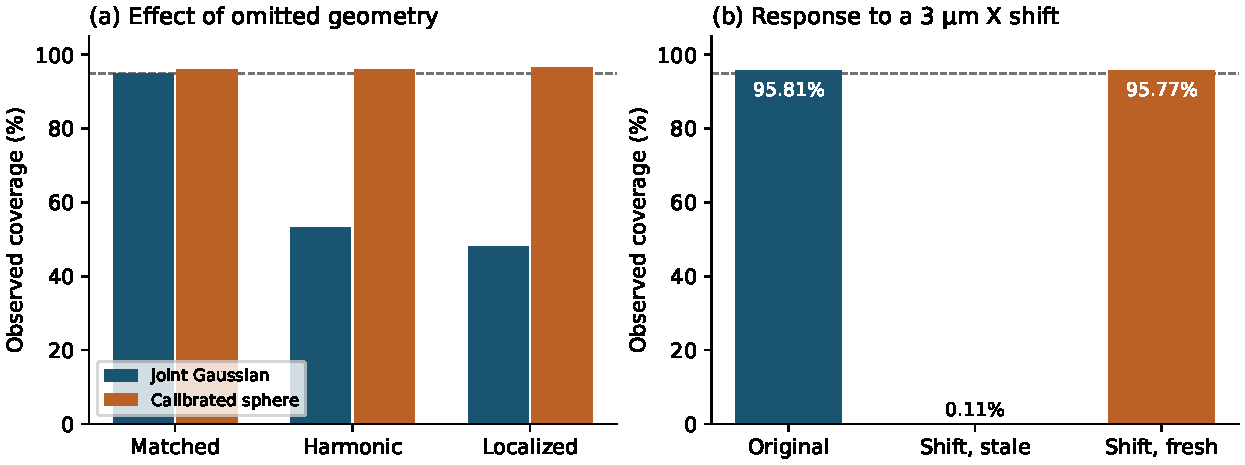
\includegraphics[width=.90\linewidth]{coverage.pdf}\par
\small \refstepcounter{figure}Figure \thefigure. Independent sensor noise. The dashed line marks 95\%. Panel (b) uses the covariance-shaped conformal region on the matched machine.\end{center}
The joint Gaussian region covers 94.98\% of measured positions under matched geometry. Omitted higher harmonics reduce coverage to 53.11\%; localized errors reduce it to 47.95\%. Nonlinear Monte Carlo gives 94.98\%, 53.12\% and 47.95\%, respectively. Both propagation methods retain the same error map. New XYZ readings reveal the larger residuals, and the calibrated sphere covers 95.86\%, 96.10\% and 96.43\% across the same cases.
 
\textbf{Correlation and region size.} Under matched geometry, assuming independent channels gives 92.57\% coverage when the simulated channels are correlated; using their known correlation gives 94.97\%. This comparison changes both rotary and probe correlation. In the matched correlated case, the calibrated ellipsoid has mean volume-equivalent radius 1.299~\um{}, against 1.663~\um{} for the sphere. With localized mismatch the ellipsoid is instead larger by 0.282~\um. A preferred region depends on both its coverage and its size.
 
\textbf{Inspection after a state change.} A prescribed 3~\um{} shift along X drives coverage from 95.81\% to 0.11\% with the original threshold. Repeating the 96 reference readings recovers 95.77\% by increasing the mean equivalent radius from 1.505 to 4.010~\um. The tool-position prediction still carries the shift. The inspection notebook displays standardized residuals by axis, maps alarms to A--C poses and flags missing readings separately. One stored replay contains eight injected spikes and eight dropouts in their respective cases; it illustrates the alarm logic. General detection rates require repeated independently labelled trials.
\clearpage\section{How the numerical experiments are connected}
\begin{center}\small
\begin{tabular}{@{}p{27mm}p{52mm}p{69mm}@{}}\toprule
Experiment & Controlled change & Question answered by its output\\\midrule
Known-map geometry & Supply the exact error map and change which terms the compensator uses. & Can the inverse command recover a prescribed pose when geometry is known?\\
Noisy calibration & Fit maps from independent virtual optical and ballbar readings. & How much position and orientation error remains after measurement and fitting?\\
Independent plant & Change the rotary basis, fixture poses, tool length and error realization. & Does a map learned over one revolution extrapolate to another turn?\\
Dynamic execution & Keep the path fixed and enable geometry, thermal, play and feedforward corrections in combinations. & Which mechanism dominates synchronous and normal-plane error at the tested speed?\\
Response audit & Keep the fit fixed across seven region methods and assess new probe readings. & How much of the observed error can be attributed to sensor noise, omitted geometry or changed conditions?\\\bottomrule
\end{tabular}\end{center}
\textbf{Two distances along a trajectory.} Let $e_i=p_i-p_{d,i}$ and let $t_i$ denote the unit tangent to the nominal path. Synchronous position error uses $\|e_i\|$. The local normal-plane metric uses
\[
 e_{\perp,i}=(I-t_it_i^{\mathsf T})e_i,\qquad
 E_{\perp}=\sqrt{N^{-1}\sum_i\|e_{\perp,i}\|^2}.
\]
A pure time lag on a locally straight segment contributes to synchronous error while its tangent component is removed from $e_{\perp,i}$. This sampled projection approximates contour deviation. The orientation metric measures the angle between the commanded and executed tool-axis unit vectors.

\textbf{Design for identification or design for a task.} For marginal-noise-scaled pose sensitivity $B_i$, the information of a chosen set is $F=\sum_i B_i^{\mathsf T}B_i$. D-optimal selection maximizes $\log\det F$. The task-based implementation weights coefficient uncertainty by the displacement sensitivities $H_j$ on prospective commands and seeks to reduce
\[
 \operatorname{tr}(CF^{-1}),\qquad C=\frac1m\sum_{j=1}^m H_j^{\mathsf T}H_j .
\]
A small diagonal initialization permits the greedy procedure to start before the selected poses span the parameter space. The final fit uses its unregularized scaled matrix. Both criteria describe sensitivity to measurement noise within the model basis.

\clearpage\subsection{From drive commands to independent sensor readings}
For one axis, the first-order lag model advances the state under a held command $u_k$ as
\[
 x_k=(1-\alpha)x_{k-1}+\alpha u_k,\qquad
 \alpha=1-\exp(-\Delta t/\tau).
\]
A transient test supplies an estimate of $\alpha$. Solving the same equation for the command gives $u_k^{\rm ff}=[d_k-(1-\hat\alpha)d_{k-1}]/\hat\alpha$ for a desired trajectory $d_k$. This explains the very small residual of the isolated, matched first-order drive experiment. In the more demanding integrated experiment the plant has two cascaded lag states. For a single held command, $a_i=\exp(-\Delta t/\tau_i)$ and $\tau_1\ne\tau_2$, the implemented exact update is
\begin{align*}
 x_{1,k}&=u_k+a_1(x_{1,k-1}-u_k),\\
 x_{2,k}&=u_k+a_2(x_{2,k-1}-u_k)
 +\frac{\tau_1(a_1-a_2)}{\tau_1-\tau_2}(x_{1,k-1}-u_k).
\end{align*}
The controller estimates an effective first-order response from a motor-side encoder. It cannot exactly invert both plant states. Play adds memory downstream of that encoder. For width $w$, the load position is the projection of its previous value onto $[u_k-w/2,u_k+w/2]$. A slow bidirectional scan estimates $w$ from the difference between median forward and reverse offsets.

For thermal feedforward the training matrix is $X=[\mathbf{1},T_1,T_2,T_3]$, where the columns are noisy temperature-sensor records. The controller fits $\hat\beta=X^\dagger D$ to measured displacement $D$ on a separate warm-up. The simulated machine responds to lagged temperatures and includes a cross term in vertical displacement. A fitted static temperature map therefore leaves a residual on a different heating cycle.

\textbf{One example of fair comparison.} The integrated simulator reuses the same path, initial conditions and noise realization for each combination of corrections. The inspection comparison similarly freezes its normal threshold while changing the replay case. Reusing these inputs makes differences between methods interpretable. Across independent seeds, the report first averages repeated noise draws within the seed and then compares seed means.

\textbf{Reading units and percentages.} A TCP RMS in micrometres measures distance. A region's volume-equivalent radius $r=Q\det(V)^{1/6}$ is the radius of a sphere with the same volume as the ellipsoid. Coverage is the fraction of noisy three-component responses falling inside the region. These are distinct outputs even when two of them carry the same length units.
\clearpage

\section{Geometric calibration and command generation}

\subsection{A known machine as a numerical control}

Start with a machine whose error maps are known exactly. This isolates errors in coordinate transformations and in the inverse command calculation. On the reference helix the uncorrected TCP RMS is 122.44 micrometres. Restricting the correction to five positioning channels increases it to 126.49. With the full known map the residual falls to numerical tolerance. Removing one component can undo cancellation with another.

\par{\small\textit{Implementation}\quad \file{fiveaxis.py}\enspace /\enspace \file{experiments.py}}\par

\begin{center}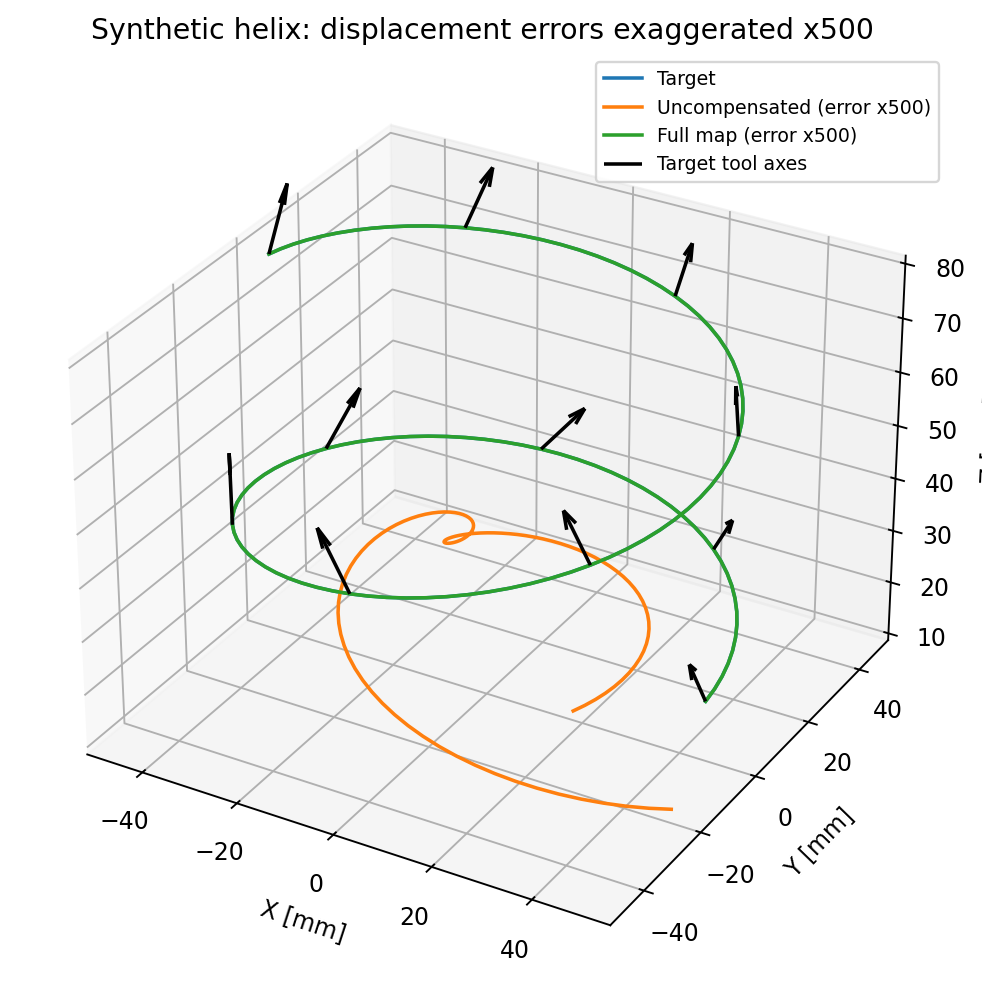
\includegraphics[width=.97\linewidth,height=73mm,keepaspectratio]{figures/helix_3d.png}\par\small\refstepcounter{figure}\textbf{Figure \thefigure.} The target and executed helix. Position differences are magnified 500 times for display.\end{center}

\begin{center}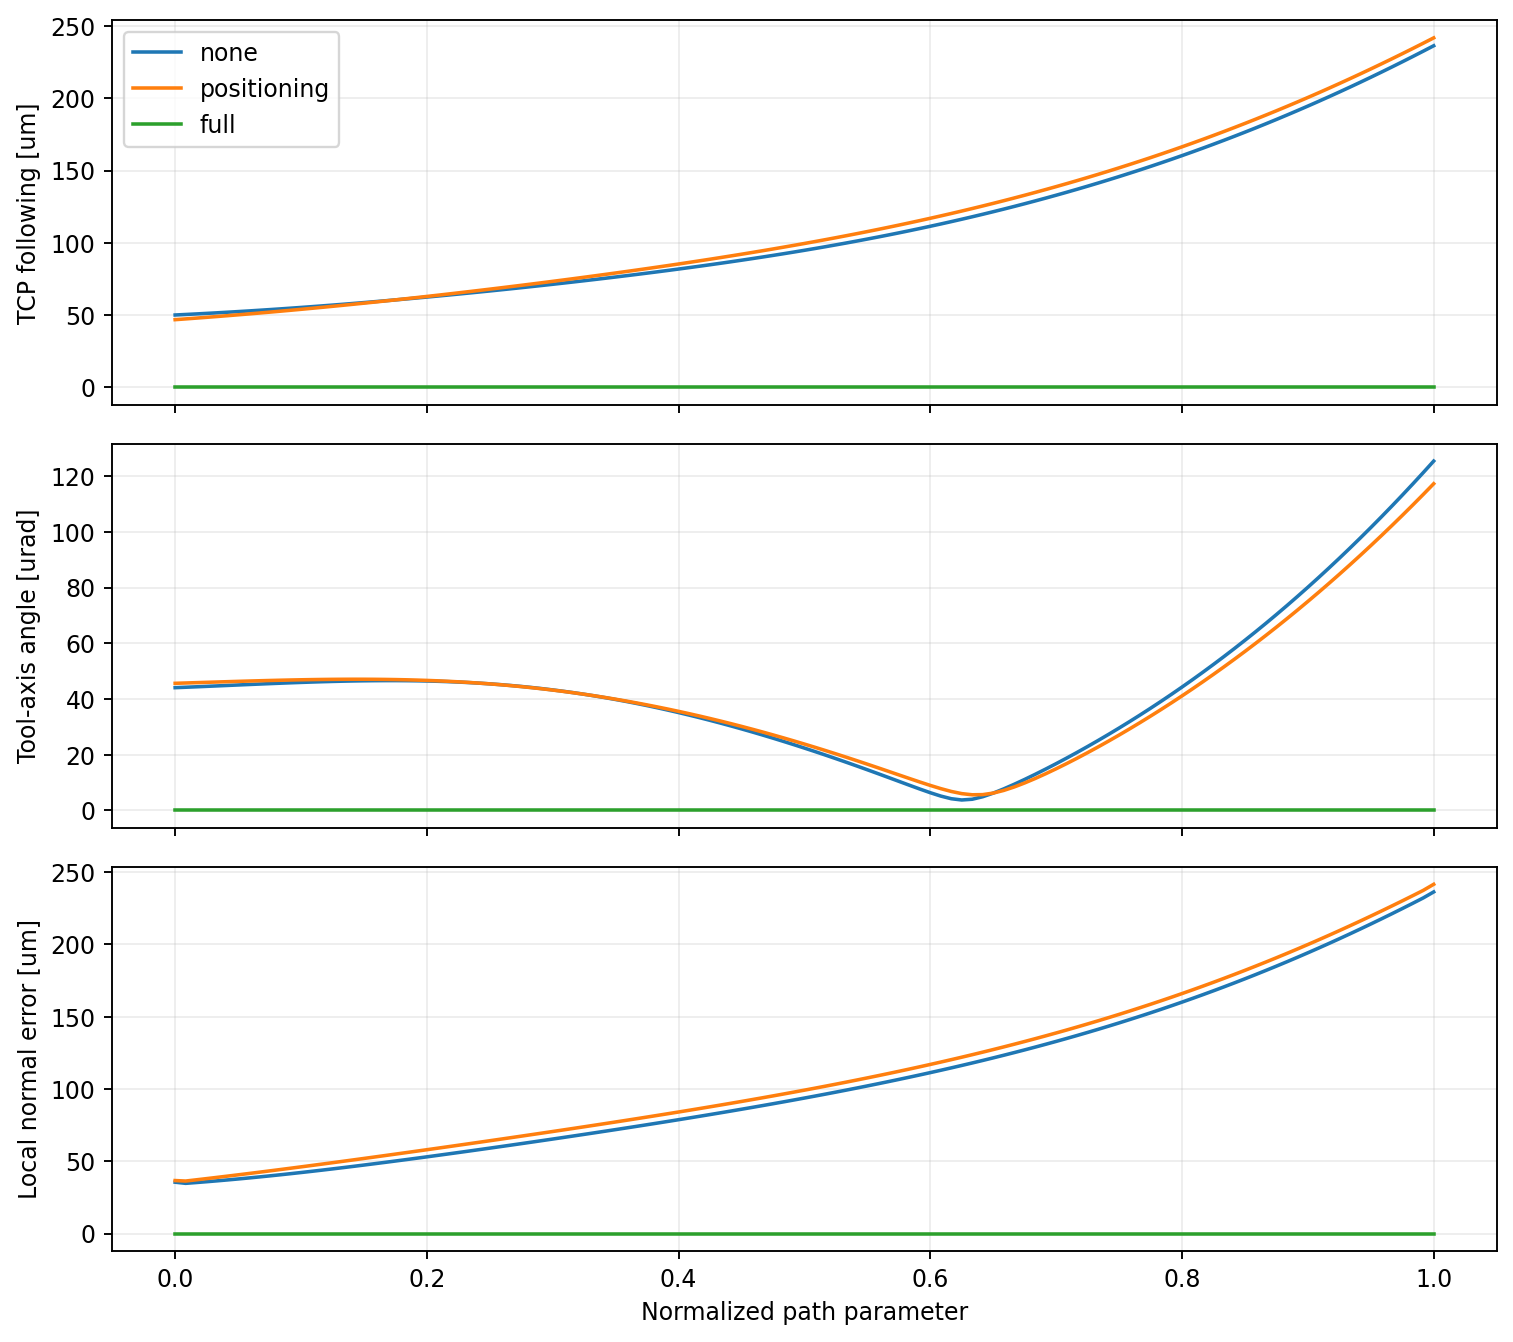
\includegraphics[width=.97\linewidth,height=73mm,keepaspectratio]{figures/geometry_compensation.png}\par\small\refstepcounter{figure}\textbf{Figure \thefigure.} TCP magnitude, axis direction and normal-plane error on the same commands.\end{center}

\clearpage

\subsection{From an axis map to a spatial error field}

An error map is referenced to a datum. Translating the part-coordinate origin changes the map evaluated at a given part position. The spatial map then holds both rotary angles fixed and samples 343 linear-axis poses. A colour records the simulated displacement norm at one pose. A single slice cannot establish a worst case for all rotary configurations.

\par{\small\textit{Implementation}\quad \file{fiveaxis.py}\enspace /\enspace \file{experiments.py}}\par

\begin{center}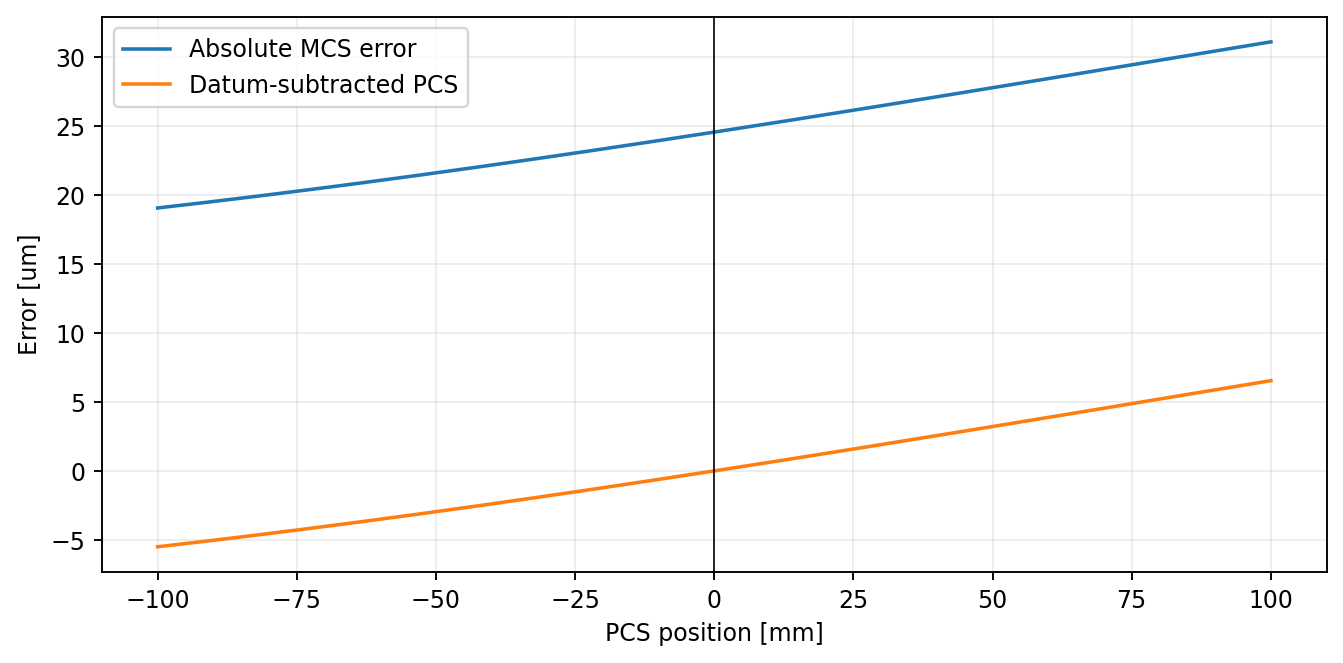
\includegraphics[width=.97\linewidth,height=73mm,keepaspectratio]{figures/pcs_mapping.png}\par\small\refstepcounter{figure}\textbf{Figure \thefigure.} Machine-coordinate and datum-relative part-coordinate maps.\end{center}

\begin{center}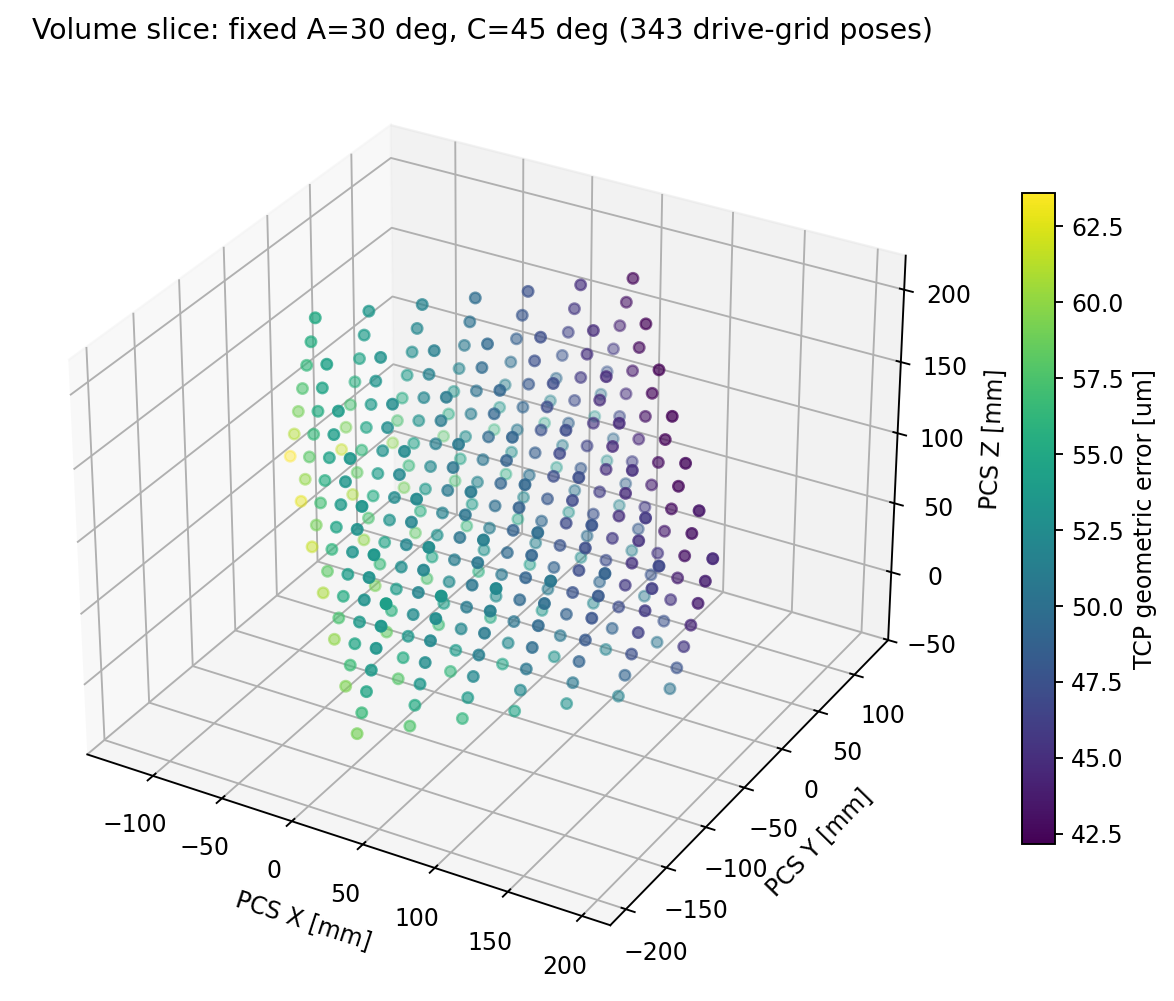
\includegraphics[width=.97\linewidth,height=73mm,keepaspectratio]{figures/volume_map.png}\par\small\refstepcounter{figure}\textbf{Figure \thefigure.} Spatial variation of TCP error at a fixed table orientation.\end{center}

\clearpage

\subsection{Sensitivity and inverse iteration}

The sensitivity sweep perturbs one geometric channel at a time and follows the same path. A small response may reflect the chosen path or the direction of the lever arm. With enlarged errors the maximum position residual drops from 1809.07 to 7.235 to 0.0167 micrometres over the first two updates. The convergence trace tests whether re-evaluating the geometry improves the command.

\par{\small\textit{Implementation}\quad \file{fiveaxis.py}\enspace /\enspace \file{experiments.py}}\par

\begin{center}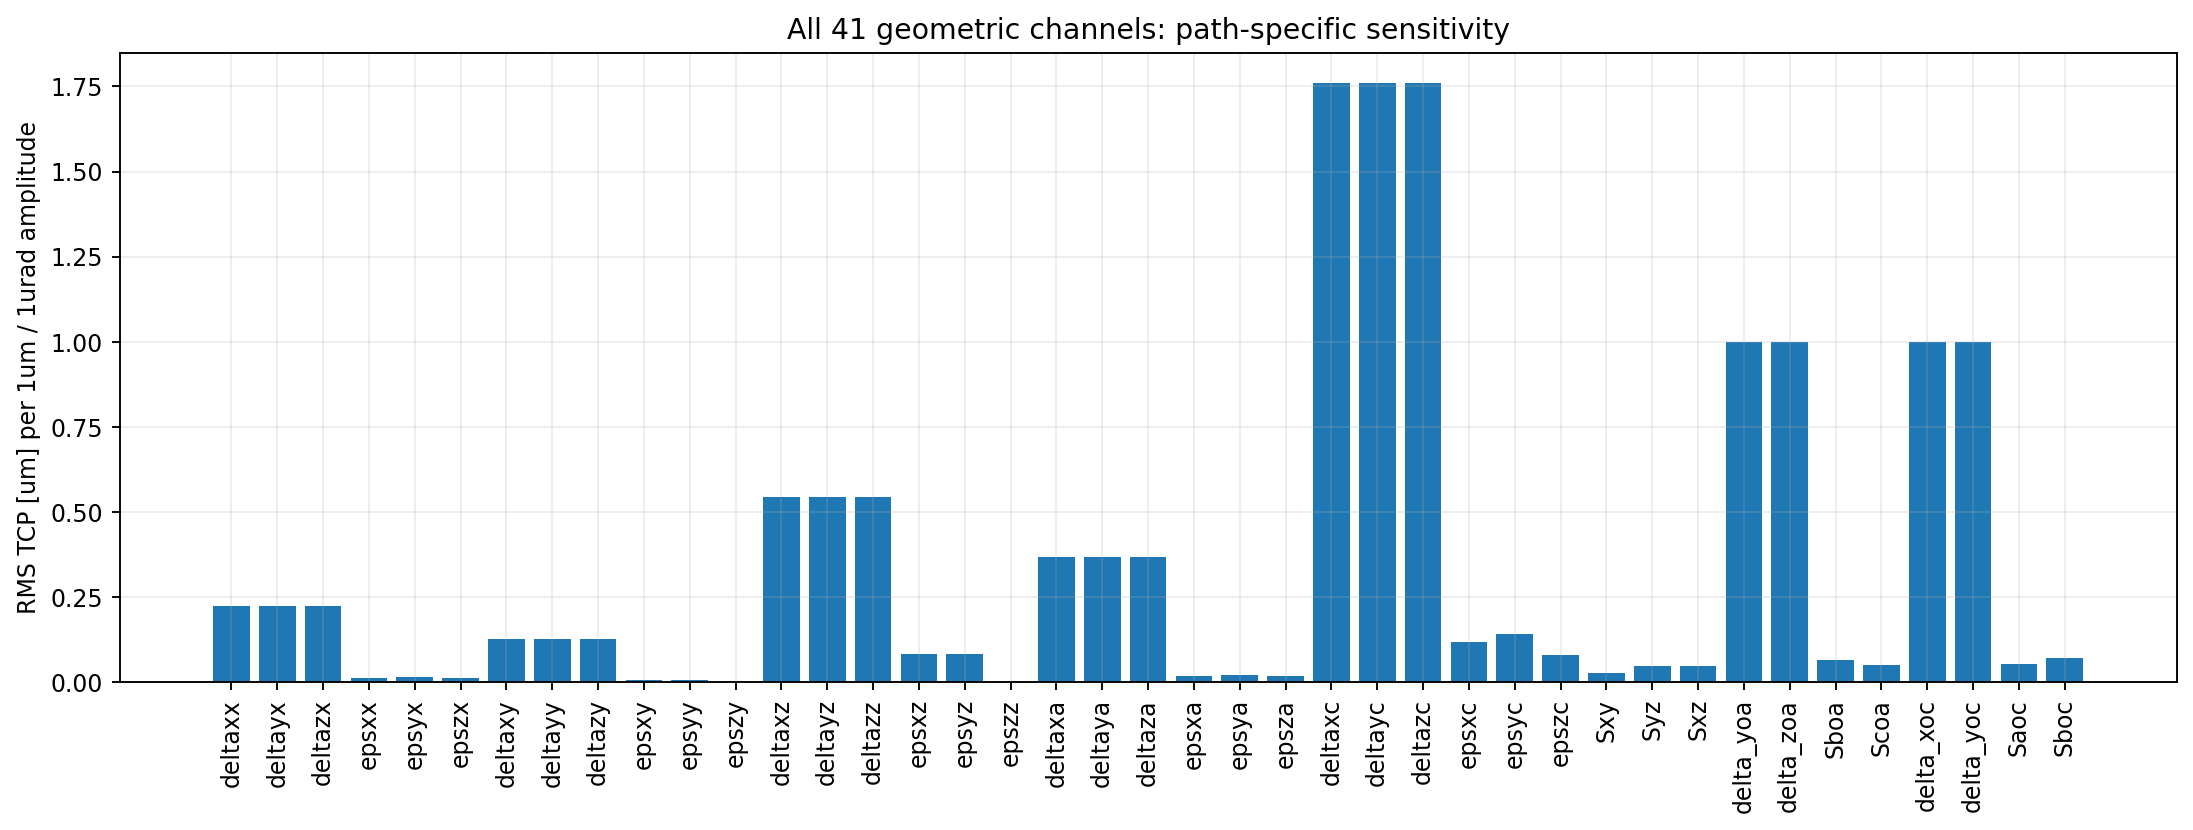
\includegraphics[width=.97\linewidth,height=73mm,keepaspectratio]{figures/sensitivity_41.png}\par\small\refstepcounter{figure}\textbf{Figure \thefigure.} Position response to each of the 30 motion-dependent and 11 fixed geometric channels.\end{center}

\begin{center}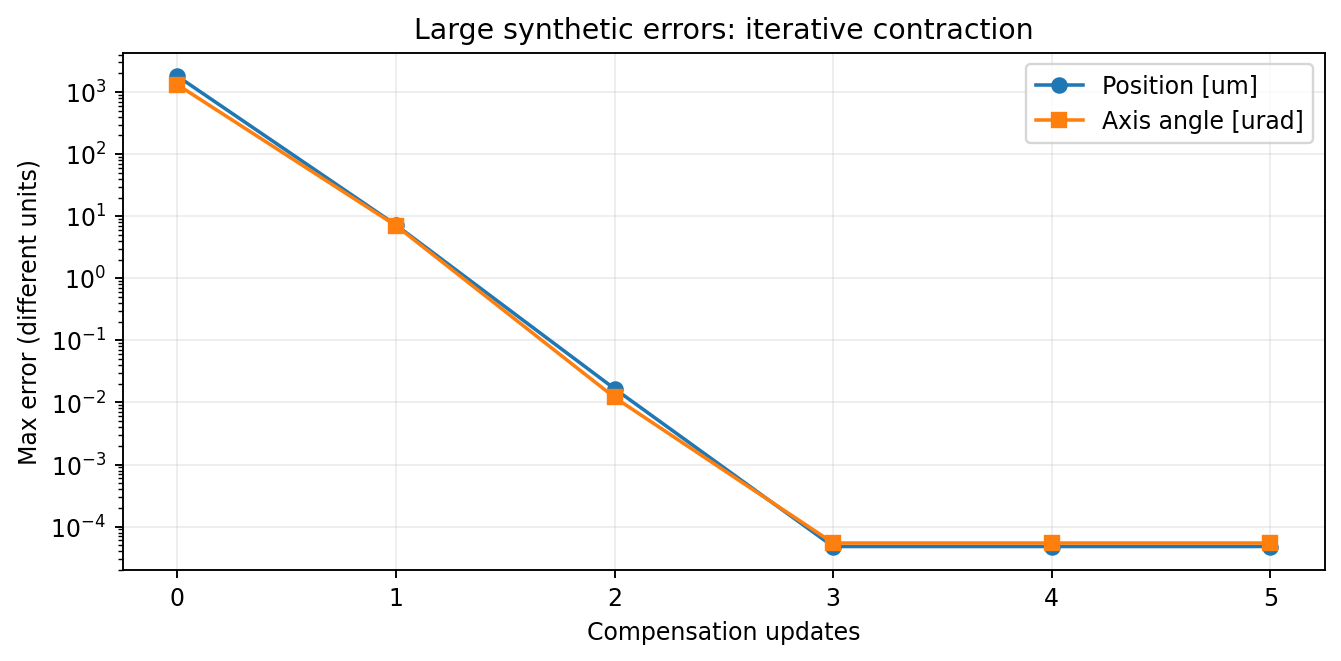
\includegraphics[width=.97\linewidth,height=73mm,keepaspectratio]{figures/iteration.png}\par\small\refstepcounter{figure}\textbf{Figure \thefigure.} Maximum residual versus compensation iteration in the enlarged-error test.\end{center}

\clearpage

\subsection{Fixture geometry and the rotary inverse}

Two readings at heights $H,H_1$ isolate A-axis tilt through $\epsilon_x=-(t_1-t_0)/(H_1-H)$, where $t$ is the tangential reading. A displaced radius $L$ supplies a second angular lever. In the noise-free implementation check, a true $+30$ microradian tilt returns $-30$ with the literal printed inverse; the corrected inverse recovers the input. The scaled condition number drops from 32,724 at 0.01 mm height separation to 5.66 at 100 mm.

\par{\small\textit{Implementation}\quad \file{calibration.py}\enspace /\enspace \file{tests/verify.py}}\par

\begin{center}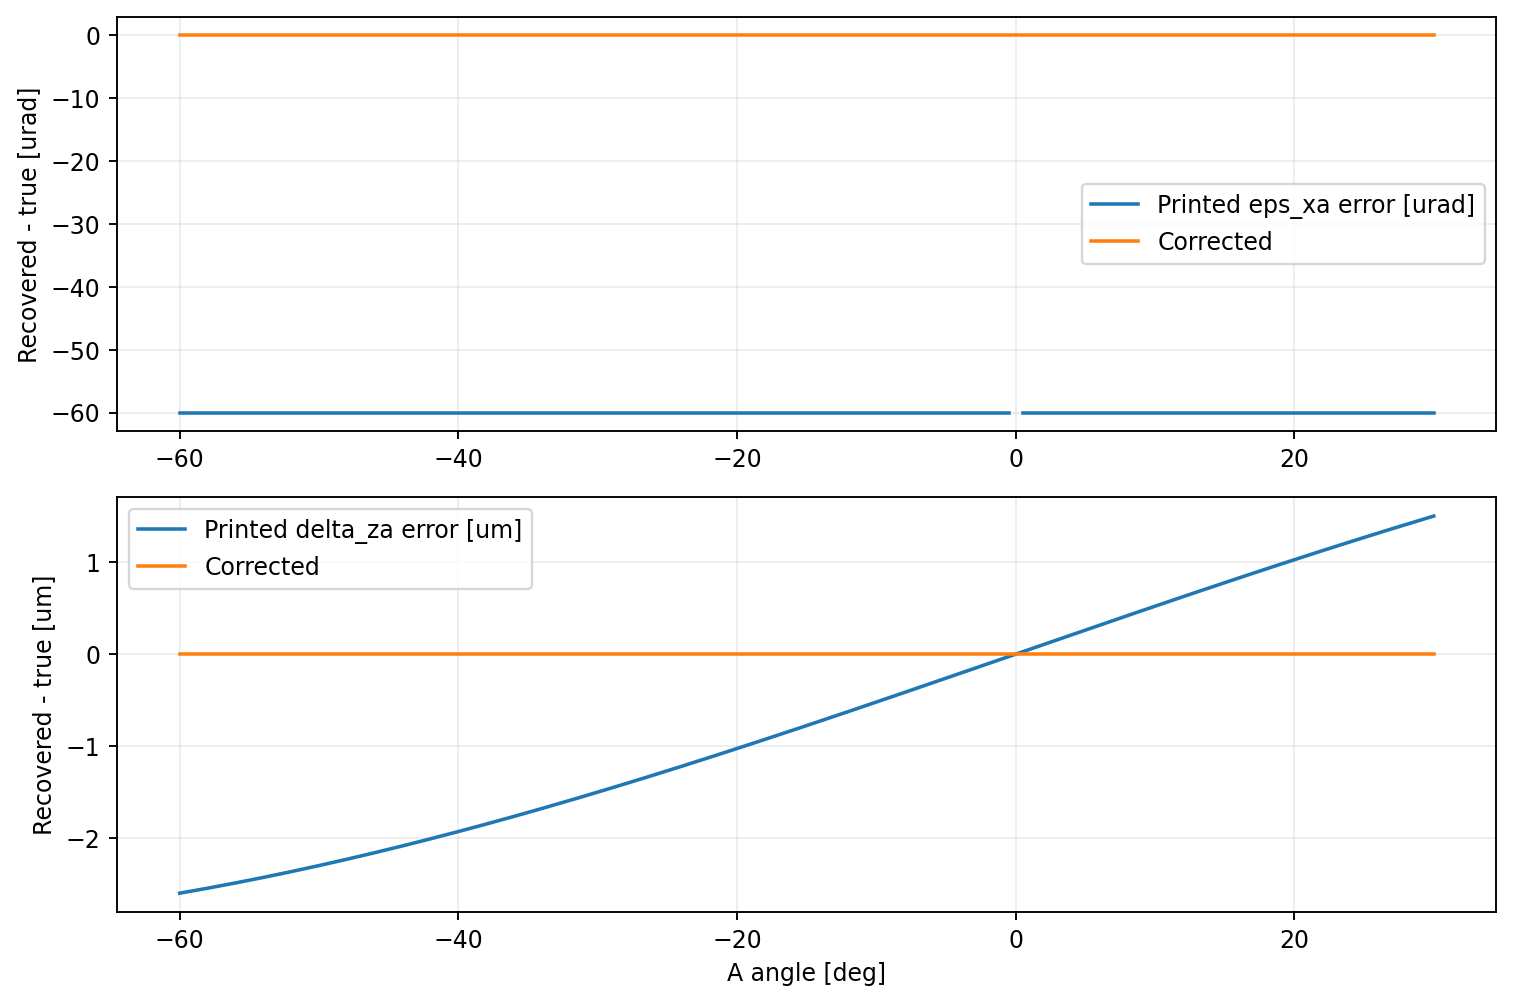
\includegraphics[width=.97\linewidth,height=73mm,keepaspectratio]{figures/eq29_audit.png}\par\small\refstepcounter{figure}\textbf{Figure \thefigure.} Literal and rederived inverses applied to measurements generated by the same forward equations.\end{center}

\begin{center}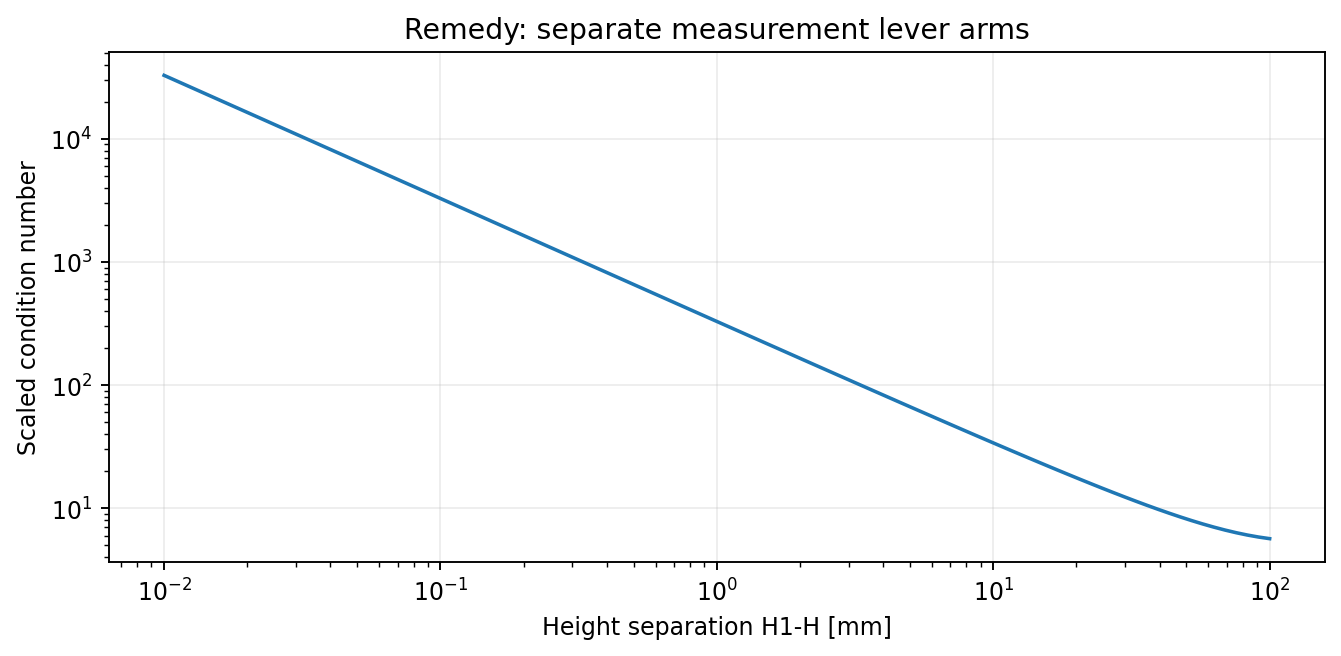
\includegraphics[width=.97\linewidth,height=73mm,keepaspectratio]{figures/calibration_geometry.png}\par\small\refstepcounter{figure}\textbf{Figure \thefigure.} Noise amplification is most severe as the two fixture heights coincide.\end{center}

\clearpage

\subsection{Identifying fixed and moving rotary errors}

Each row of the calibration matrix projects a displacement sensitivity along the ballbar direction. The full three-direction design resolves 44 of 44 parameters in this baseline. Radial readings alone resolve 40. The alternating fit cycles between fixed alignment and motion-dependent coefficients; residual convergence measures agreement with the measurements, while weak parameter directions can remain uncertain.

\par{\small\textit{Implementation}\quad \file{calibration.py}\enspace /\enspace \file{experiments.py}}\par

\begin{center}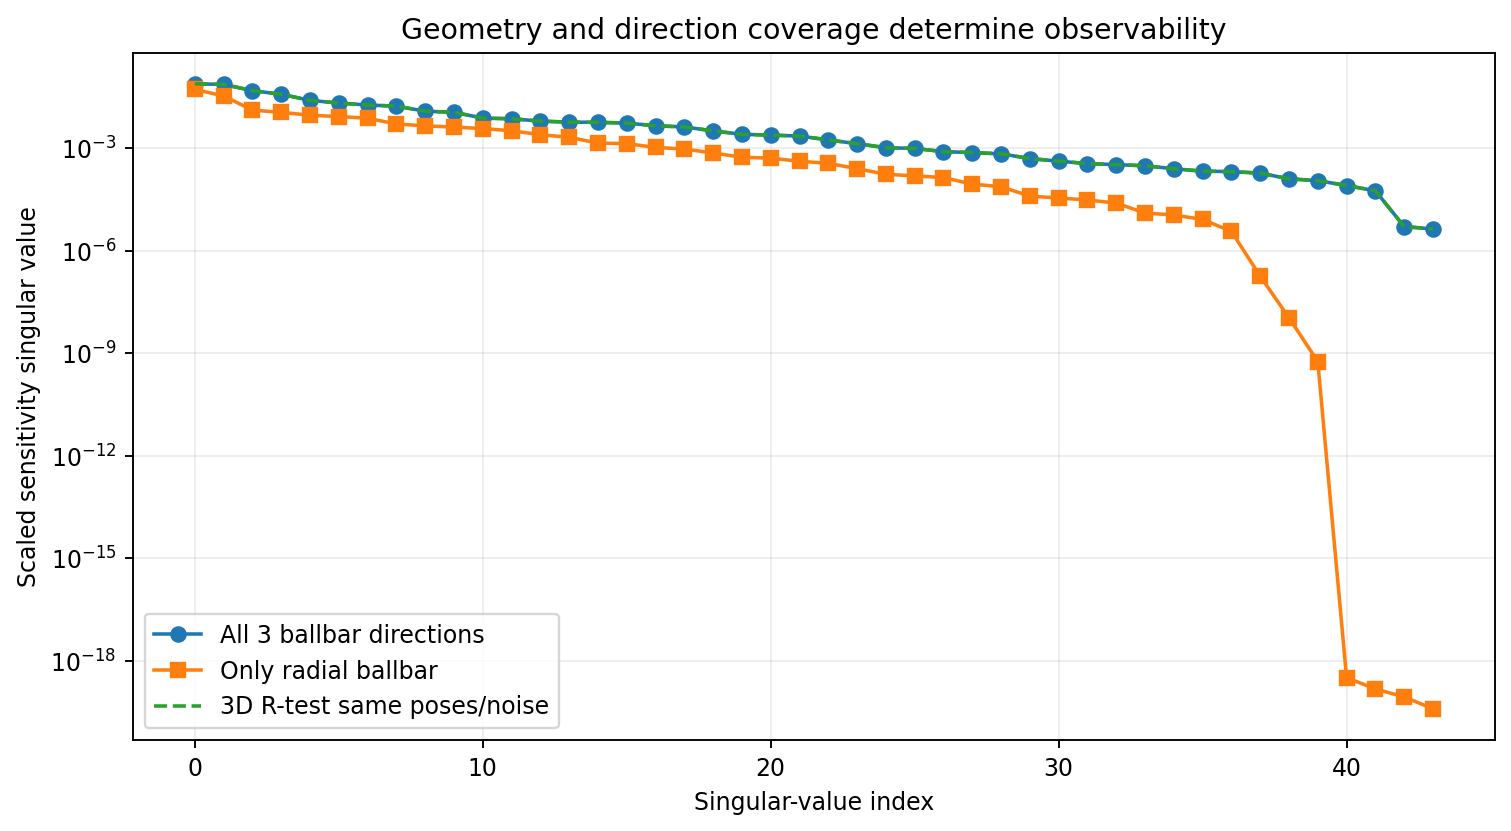
\includegraphics[width=.97\linewidth,height=73mm,keepaspectratio]{figures/observability.png}\par\small\refstepcounter{figure}\textbf{Figure \thefigure.} Singular spectra for complete, radial-only and Cartesian observation systems.\end{center}

\begin{center}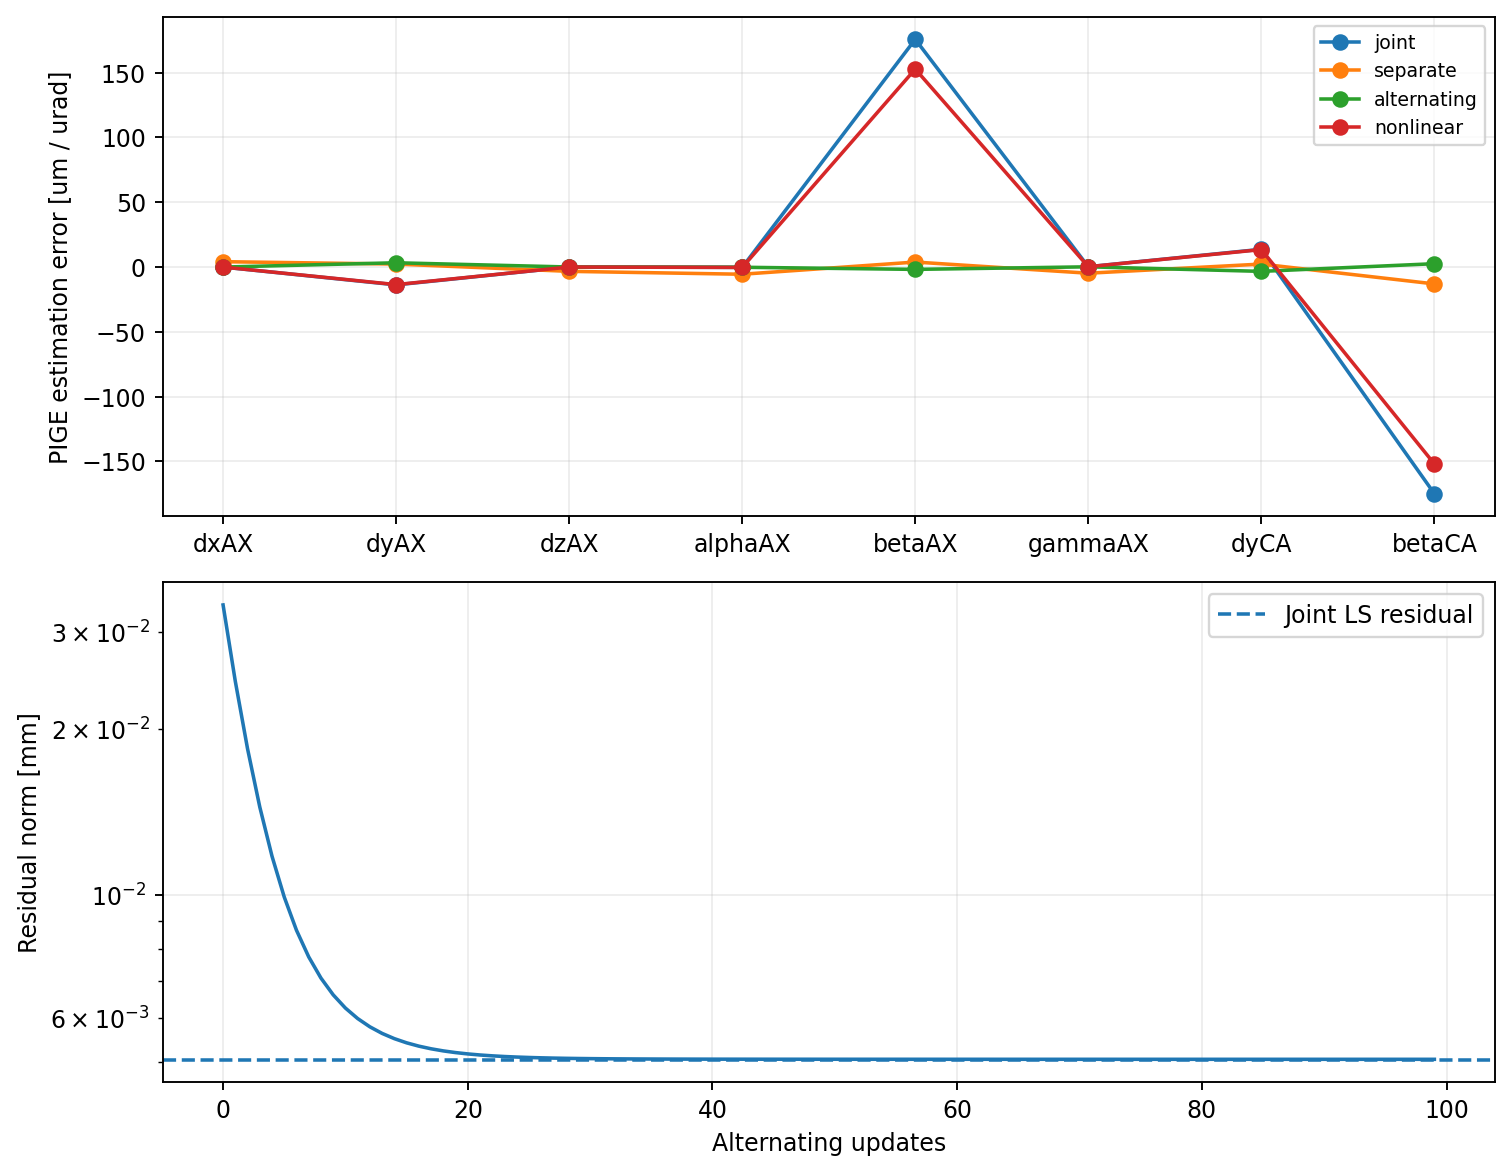
\includegraphics[width=.97\linewidth,height=73mm,keepaspectratio]{figures/pige_decoupling.png}\par\small\refstepcounter{figure}\textbf{Figure \thefigure.} Fixed alignment estimates and residual history during alternating fits.\end{center}

\clearpage

\subsection{What the fitted rotary maps look like}

The figures compare the six components per rotary axis. On held-out sensor readings, joint, alternating and nonlinear fits give RMS errors of 0.0582, 0.0575 and 0.0550 micrometres, respectively. Their normalized parameter RMSEs are 8.60, 1.30 and 7.89. Similar predicted sensor traces can arise from substantially different coefficients.

\par{\small\textit{Implementation}\quad \file{calibration.py}\enspace /\enspace \file{experiments.py}}\par

\begin{center}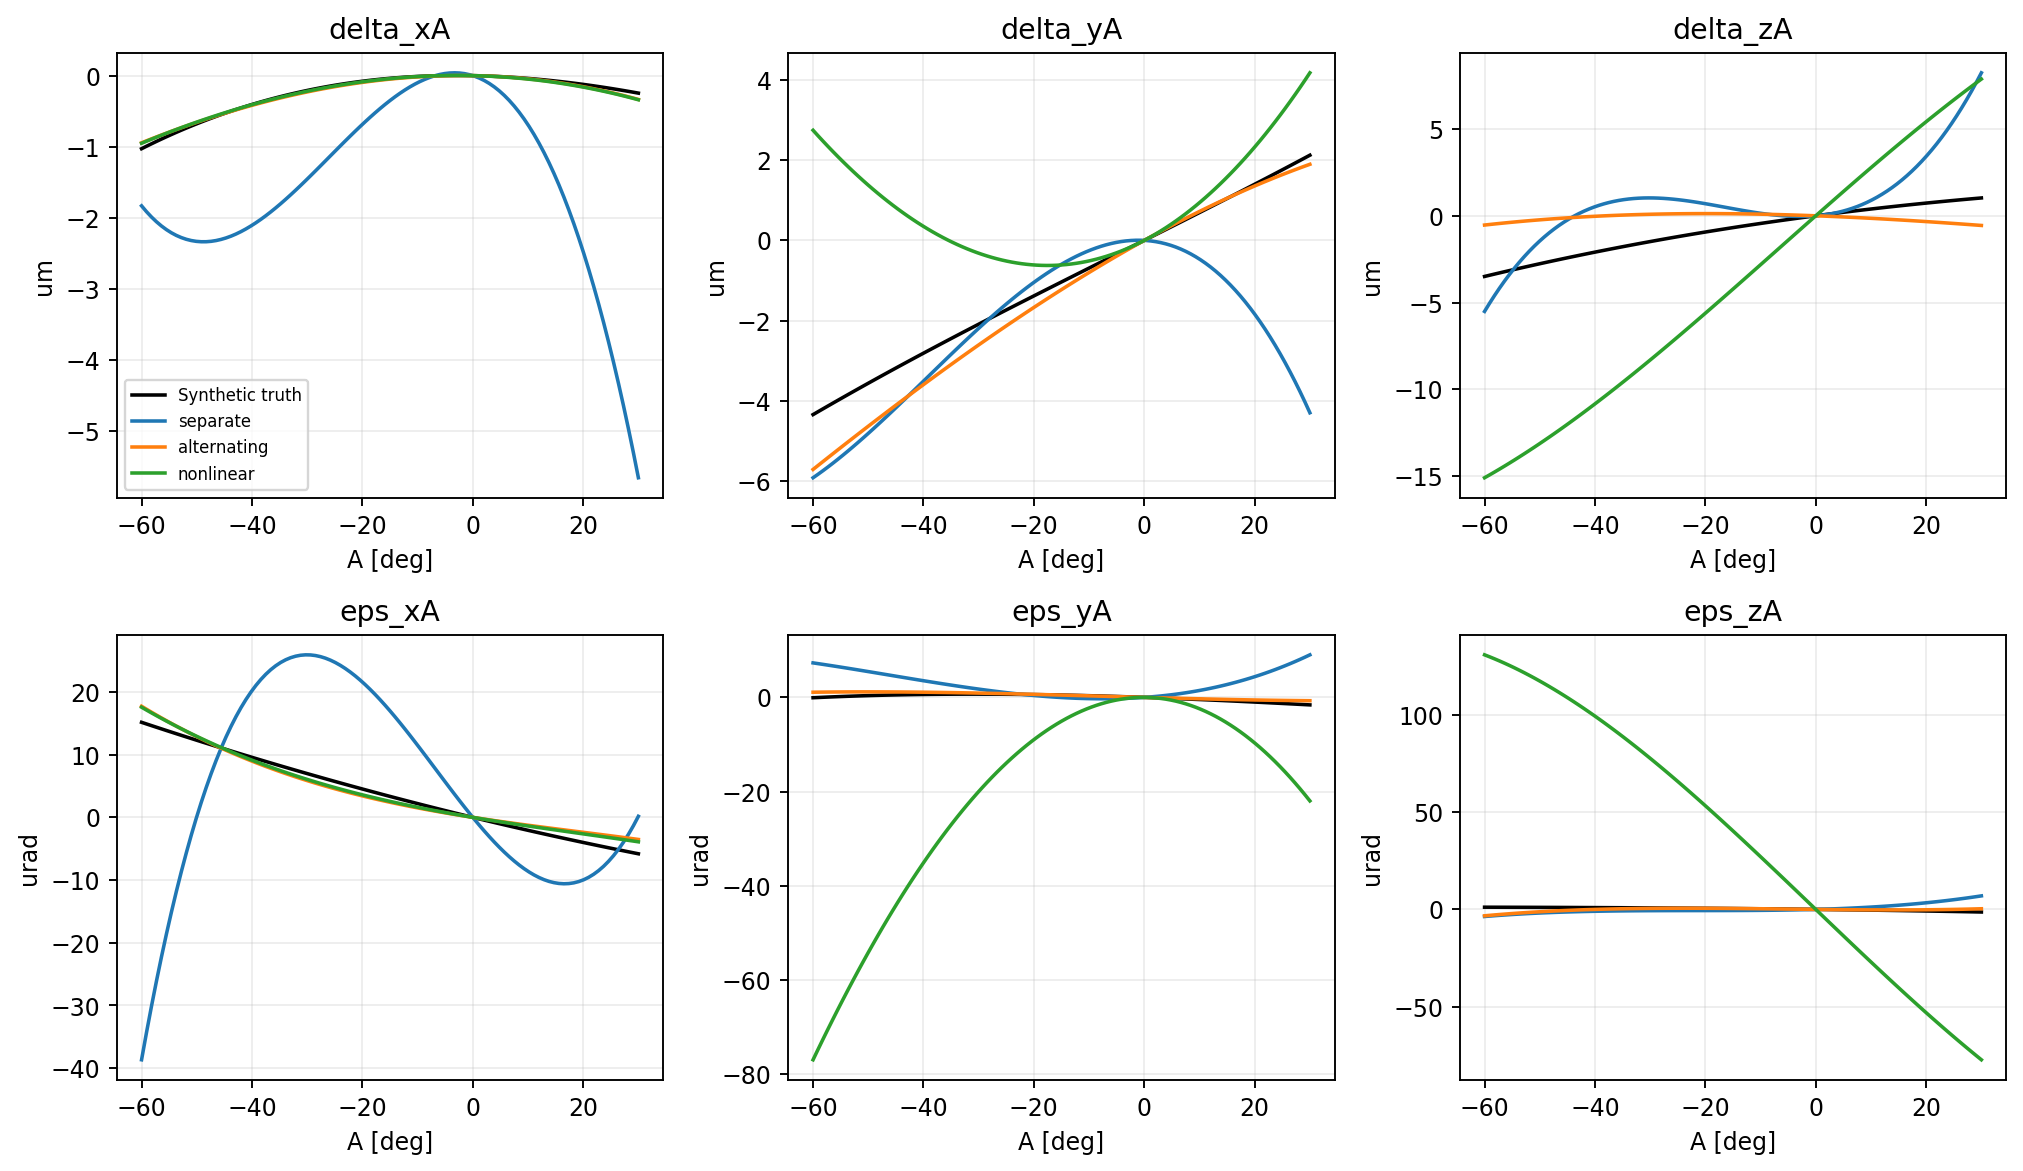
\includegraphics[width=.97\linewidth,height=73mm,keepaspectratio]{figures/rotary_pdge_A.png}\par\small\refstepcounter{figure}\textbf{Figure \thefigure.} A-axis displacement and angular maps estimated from the virtual measurements.\end{center}

\begin{center}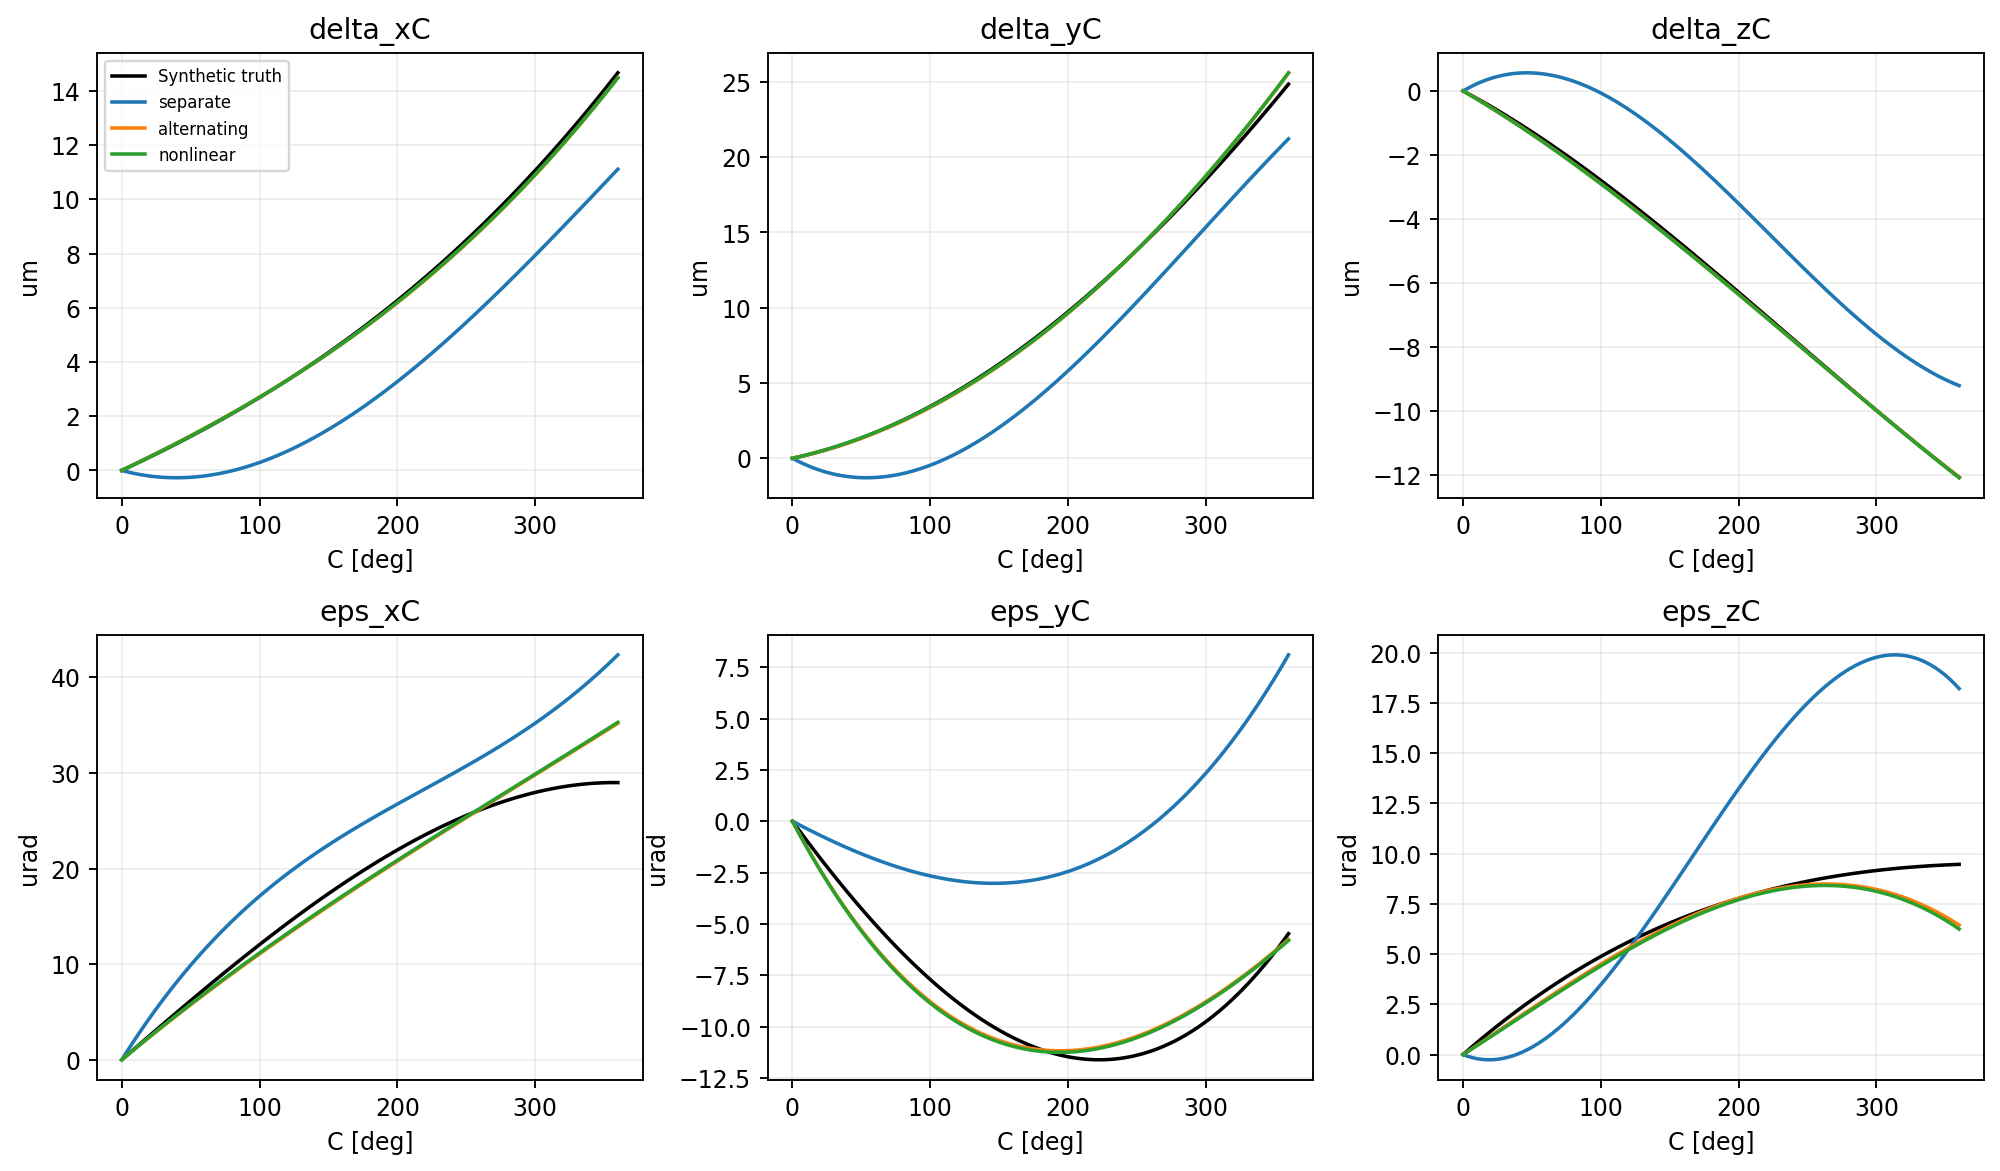
\includegraphics[width=.97\linewidth,height=73mm,keepaspectratio]{figures/rotary_pdge_C.png}\par\small\refstepcounter{figure}\textbf{Figure \thefigure.} C-axis maps from the same four estimation strategies.\end{center}

\clearpage

\subsection{Estimating the linear-axis maps}

Fitting noisy component measurements replaces the ideal exact-map control. The fitted model gives 0.861 micrometres TCP RMS on its test path. Dropping the three linear-axis roll channels raises that value to 0.929. Roll couples to position through offsets, so an angular channel with little effect in one setup can matter at another tool length or pose.

\par{\small\textit{Implementation}\quad \file{experiments.py}\enspace /\enspace \file{calibration.py}}\par

\begin{center}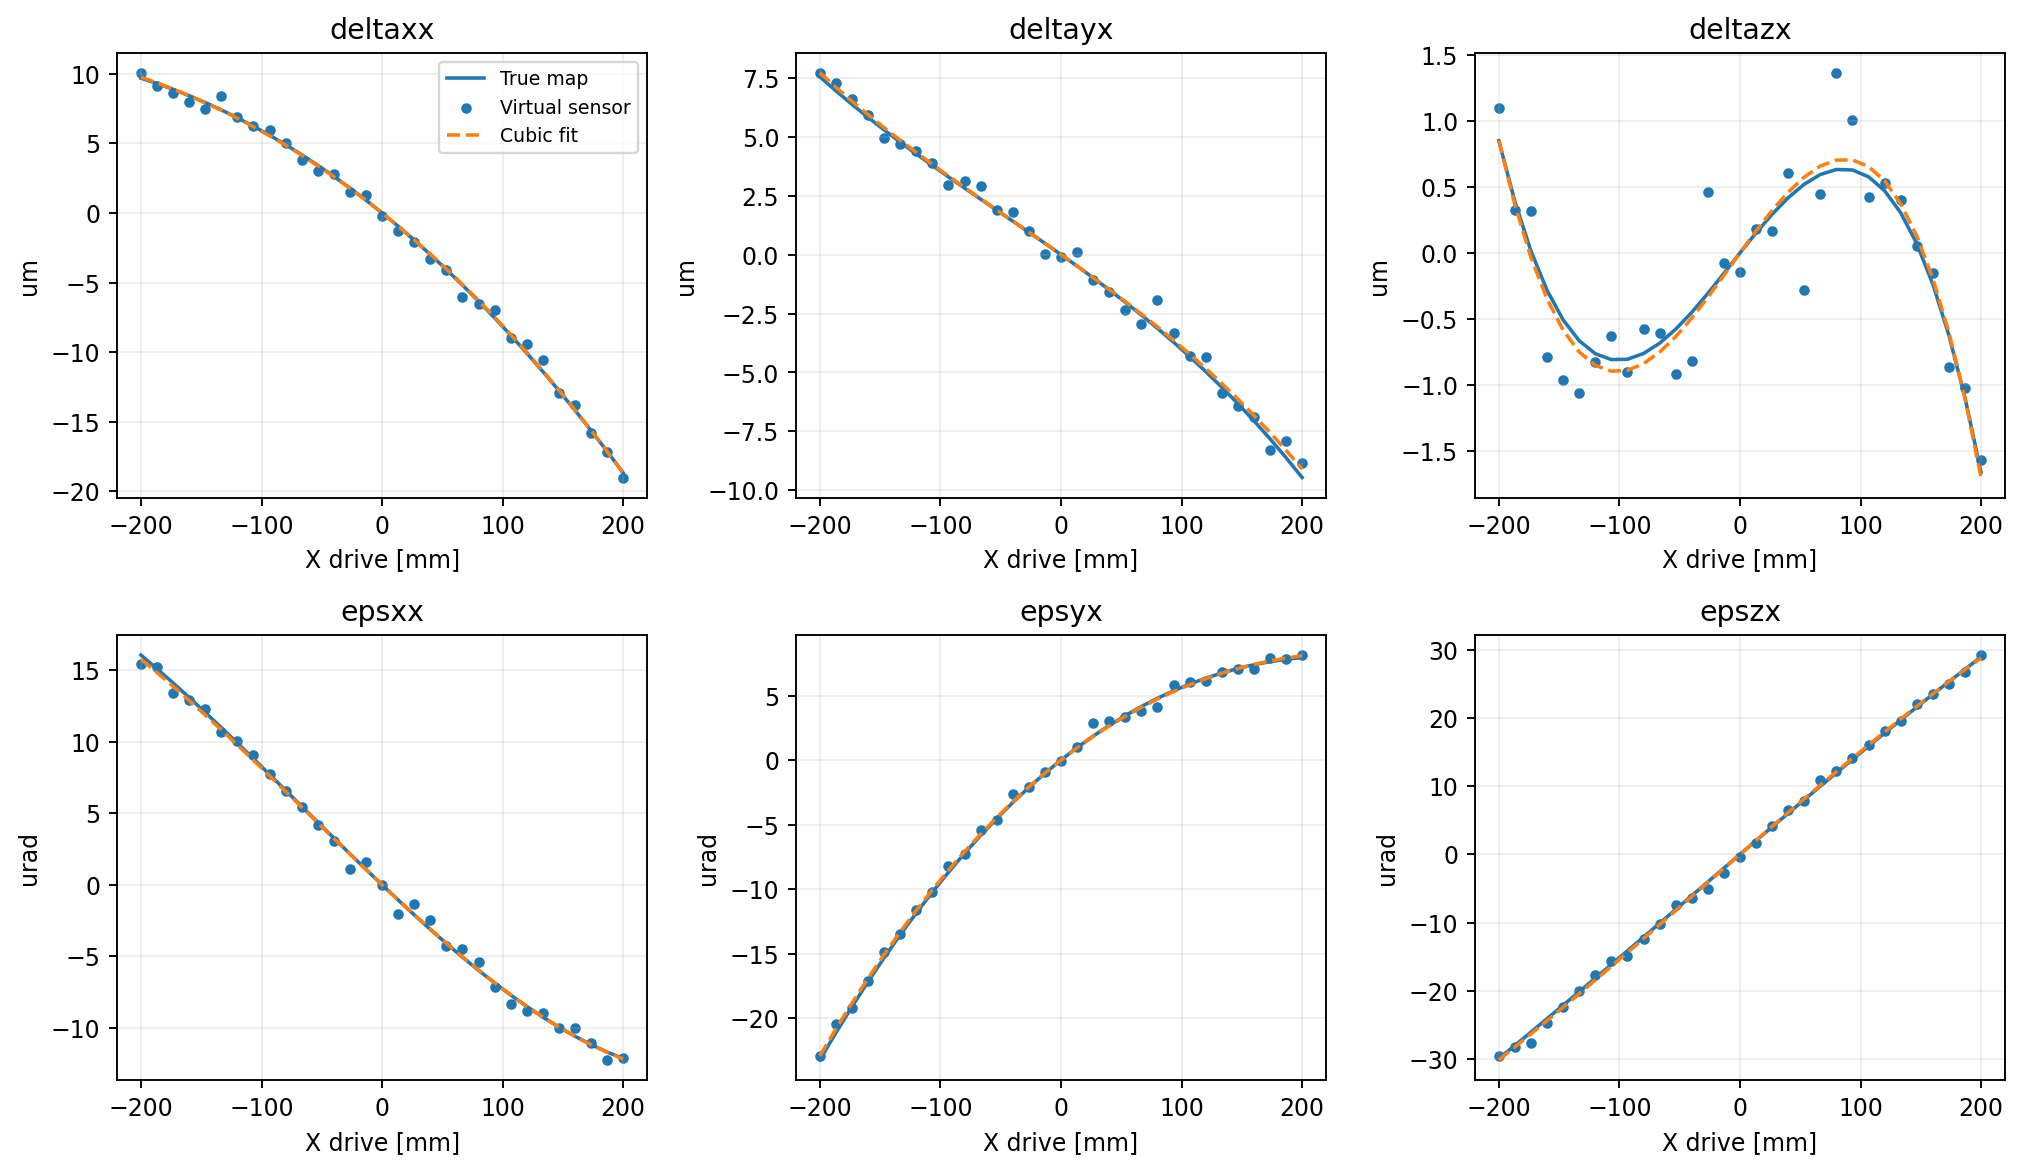
\includegraphics[width=.97\linewidth,height=73mm,keepaspectratio]{figures/linear_sensors.png}\par\small\refstepcounter{figure}\textbf{Figure \thefigure.} Six X-axis component observations, synthetic truth and fitted cubics.\end{center}

\begin{center}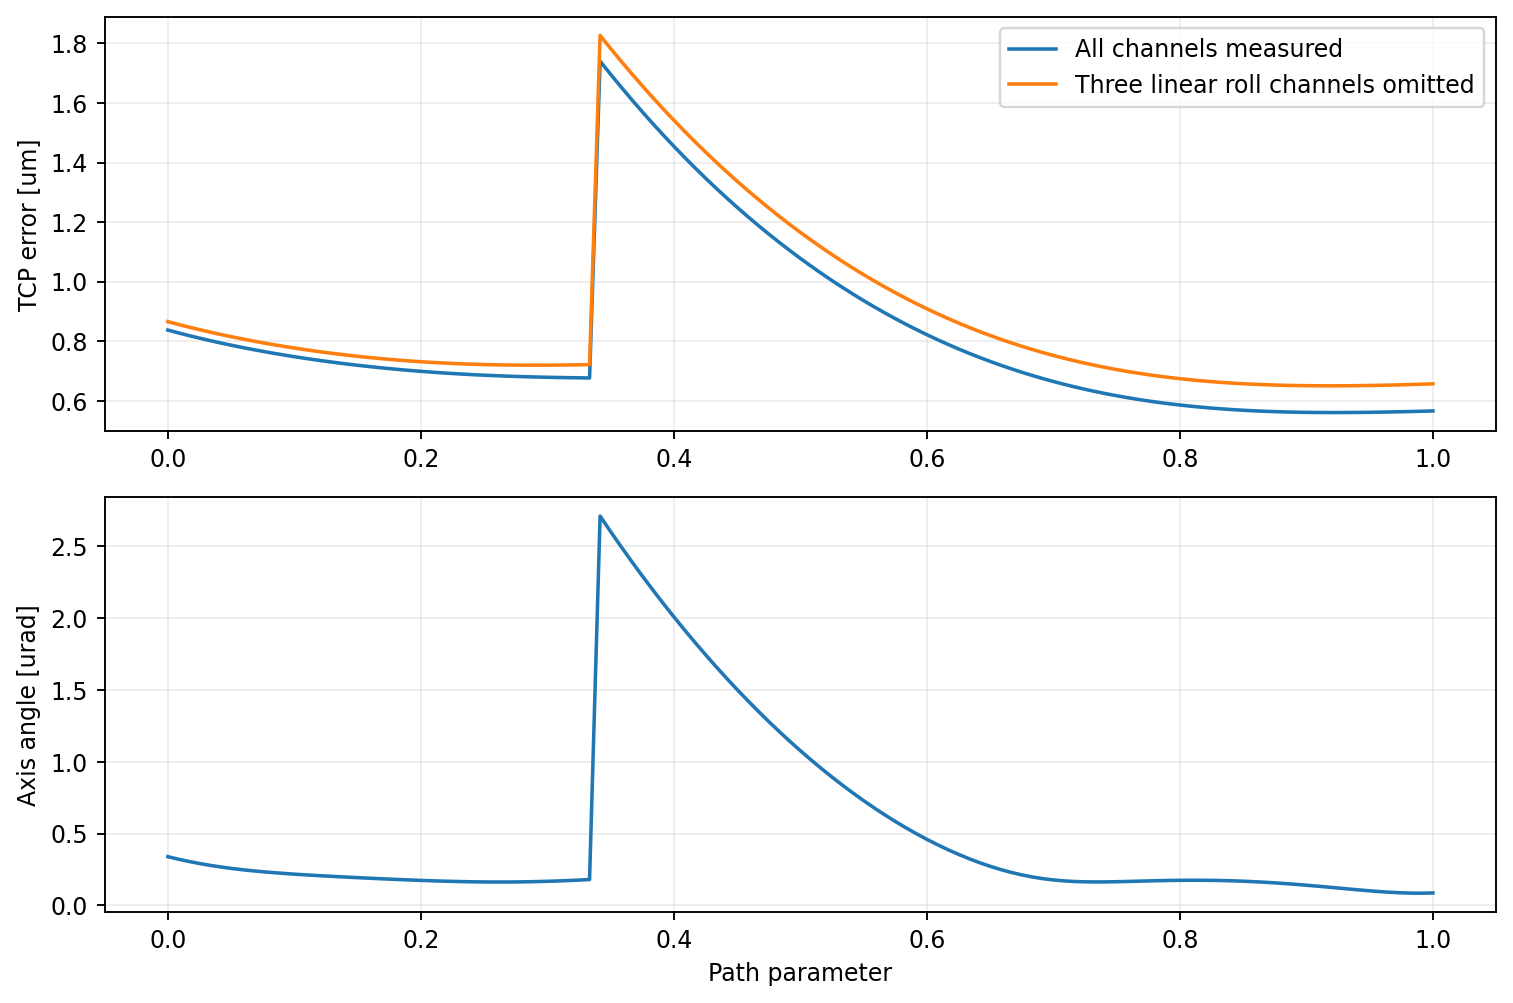
\includegraphics[width=.97\linewidth,height=73mm,keepaspectratio]{figures/roll_and_map_noise.png}\par\small\refstepcounter{figure}\textbf{Figure \thefigure.} Residuals using all fitted channels and after omitting linear-axis rolls.\end{center}

\clearpage

\subsection{Closing the loop from measurement to motion}

The model estimated from optical and ballbar data is applied to a different trajectory. TCP RMS falls from 92.442 to 0.546 micrometres and axis RMS from 58.483 to 7.823 microradians. Ballbar traces below provide a second view: a probe observes a projection of the geometric change and adds measurement noise. A small axial ballbar signal alone cannot certify the vector TCP error.

\par{\small\textit{Implementation}\quad \file{experiments.py}\enspace /\enspace \file{io_tools.py}}\par

\begin{center}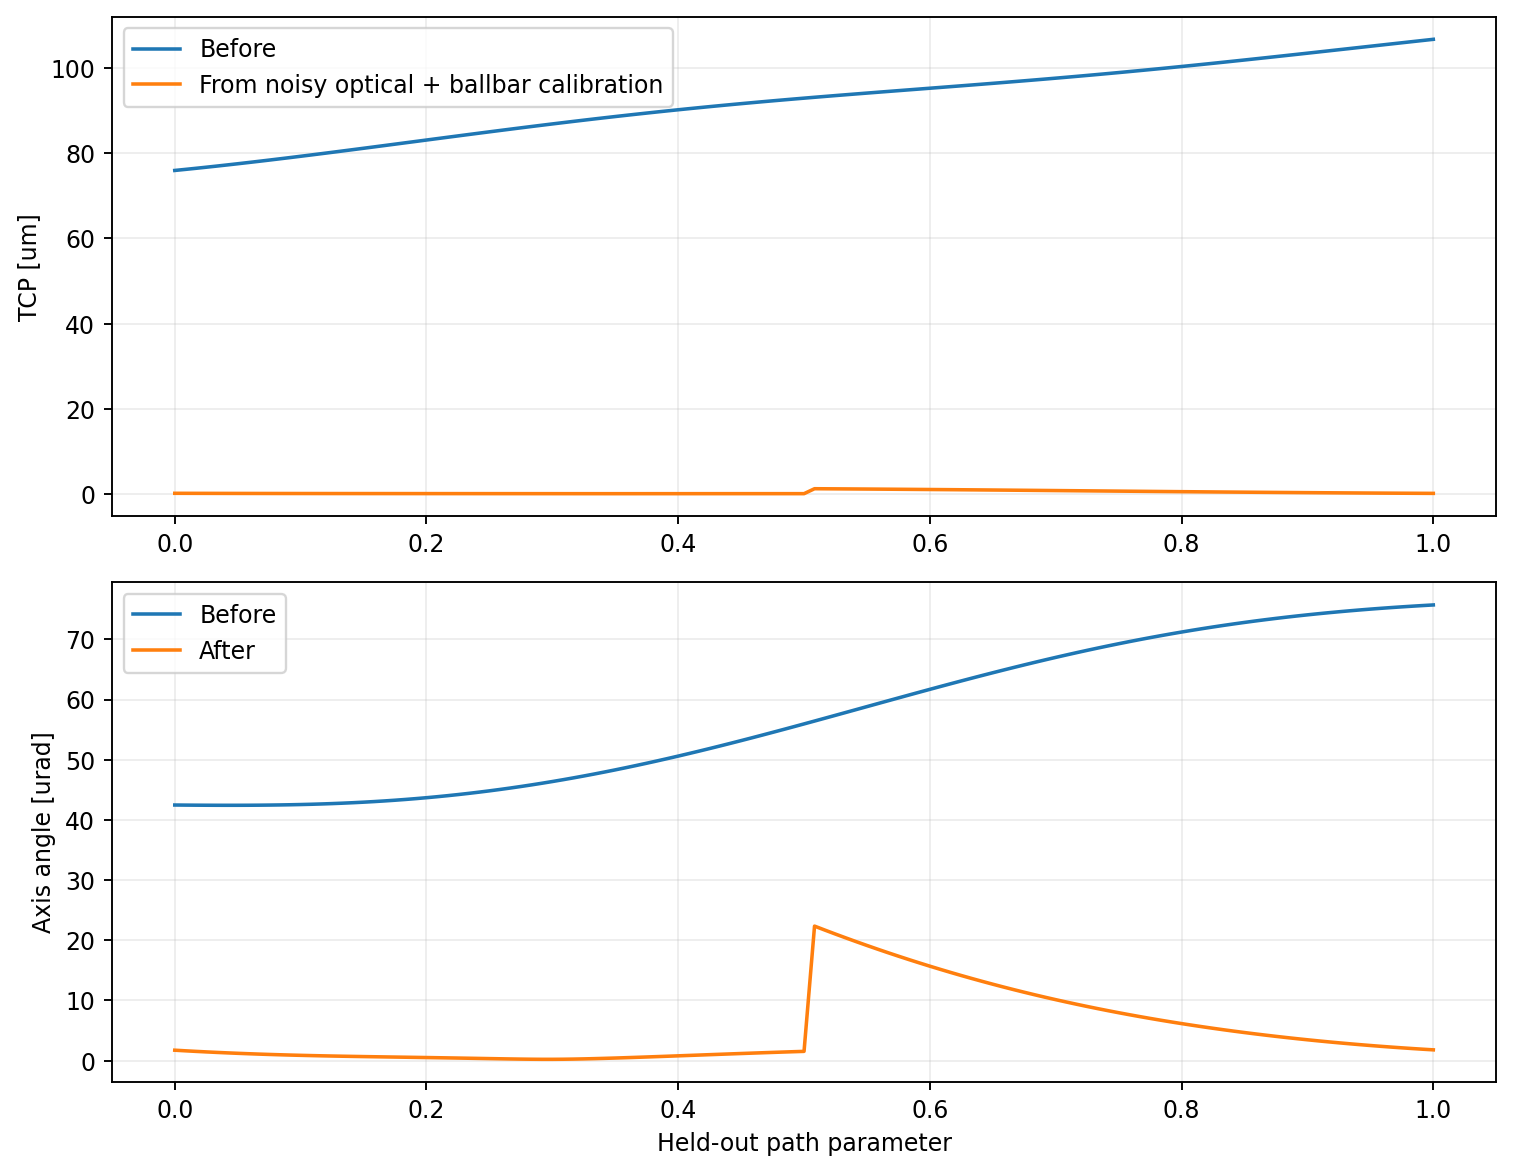
\includegraphics[width=.97\linewidth,height=73mm,keepaspectratio]{figures/calibration_to_compensation.png}\par\small\refstepcounter{figure}\textbf{Figure \thefigure.} Held-out TCP and orientation residuals before and after fitting the machine.\end{center}

\begin{center}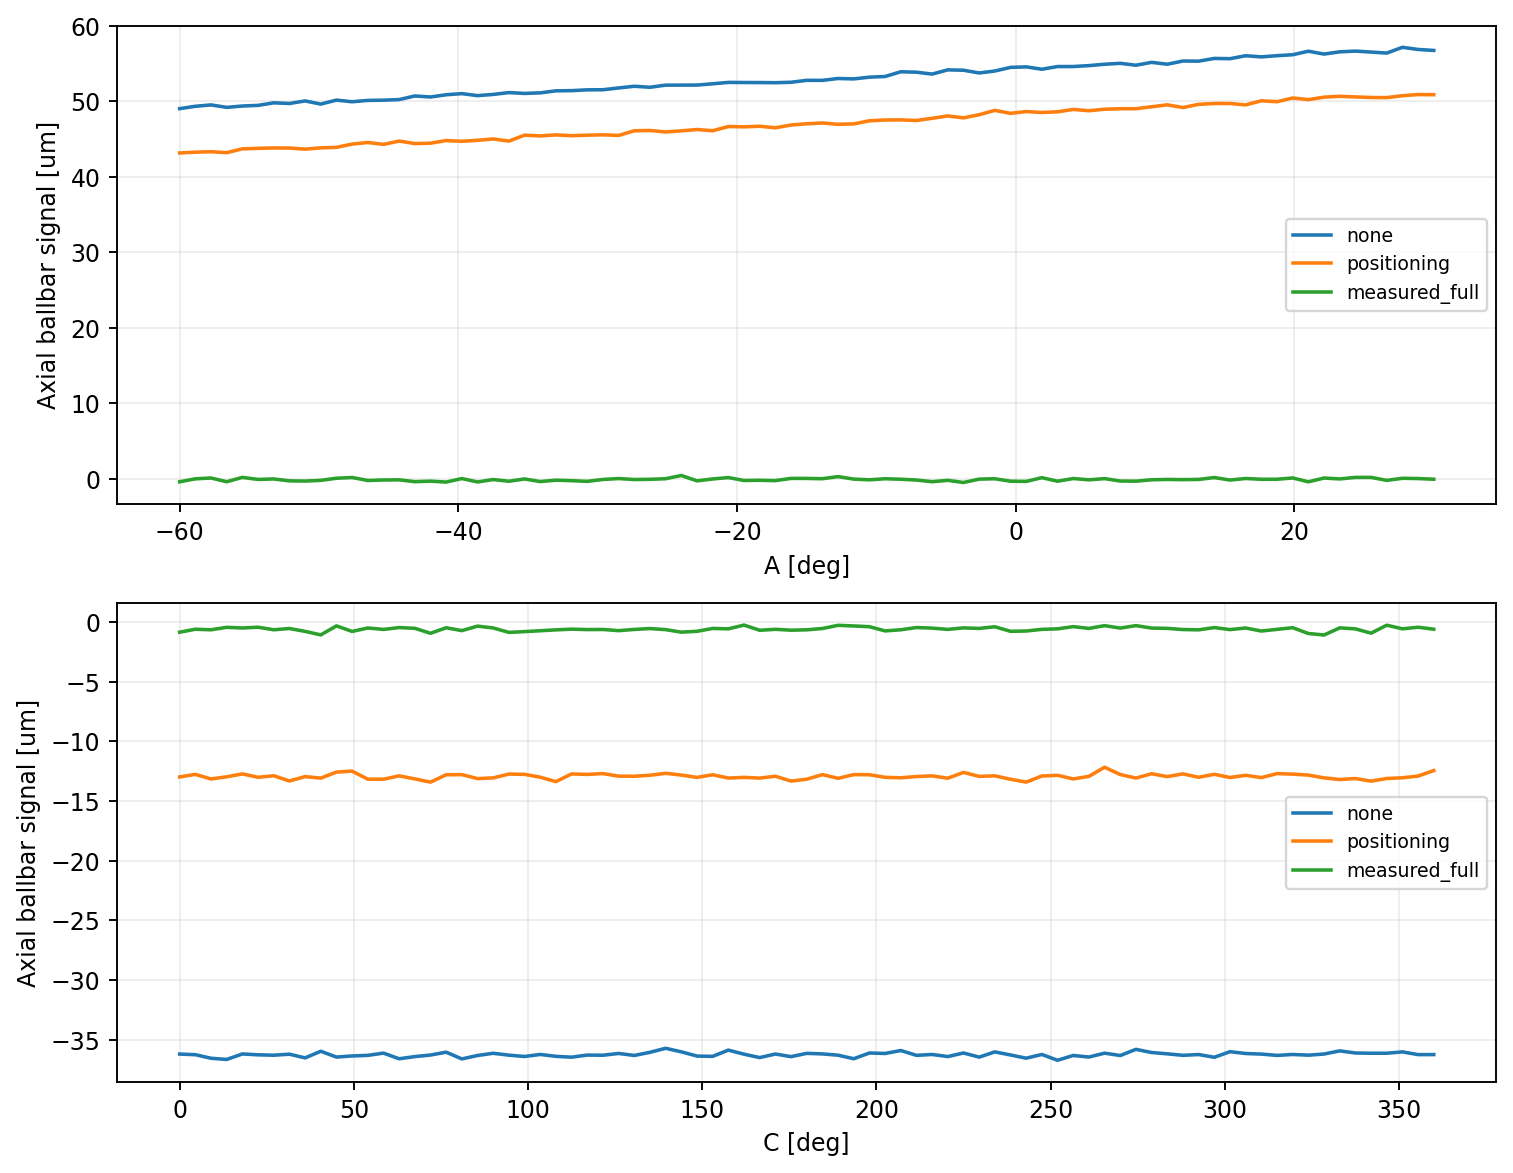
\includegraphics[width=.97\linewidth,height=73mm,keepaspectratio]{figures/ballbar_compensation.png}\par\small\refstepcounter{figure}\textbf{Figure \thefigure.} Virtual axial ballbar measurements before and after correction.\end{center}

\clearpage

\subsection{When a calibration becomes ill-conditioned}

The baseline coefficient-standard-deviation vector differs by 1.37\% from its 100-trial linear-noise prediction. That check concerns a specified calibration design. A separate singularity arises in the inverse motion: when the tool approaches the C-axis direction, azimuth becomes poorly determined. The scaled task-Jacobian condition rises from 2.79 at $60^\circ$ tilt to roughly 448,000 at $0.001^\circ$. Branch continuity helps choose commands across this region.

\par{\small\textit{Implementation}\quad \file{experiments.py}\enspace /\enspace \file{fiveaxis.py}}\par

\begin{center}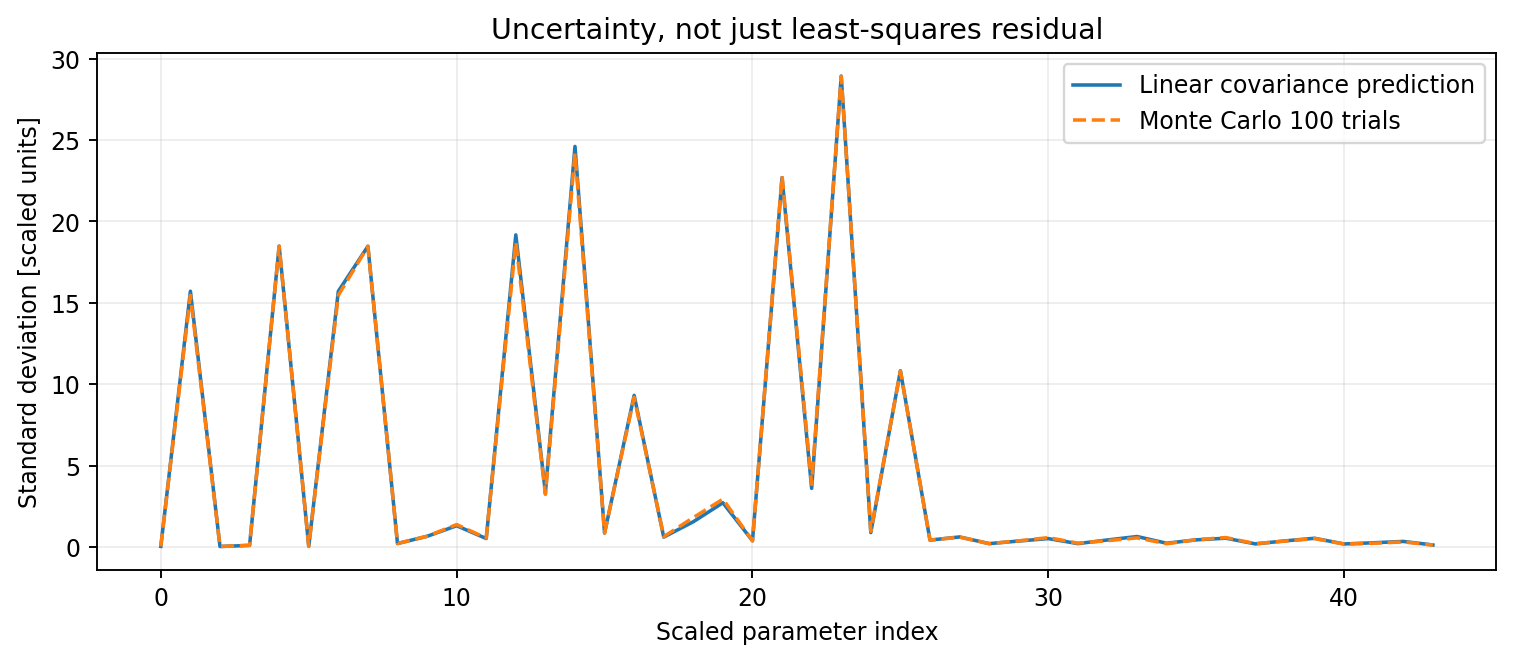
\includegraphics[width=.97\linewidth,height=73mm,keepaspectratio]{figures/uncertainty.png}\par\small\refstepcounter{figure}\textbf{Figure \thefigure.} Analytic parameter standard deviations and repeated calibration estimates.\end{center}

\begin{center}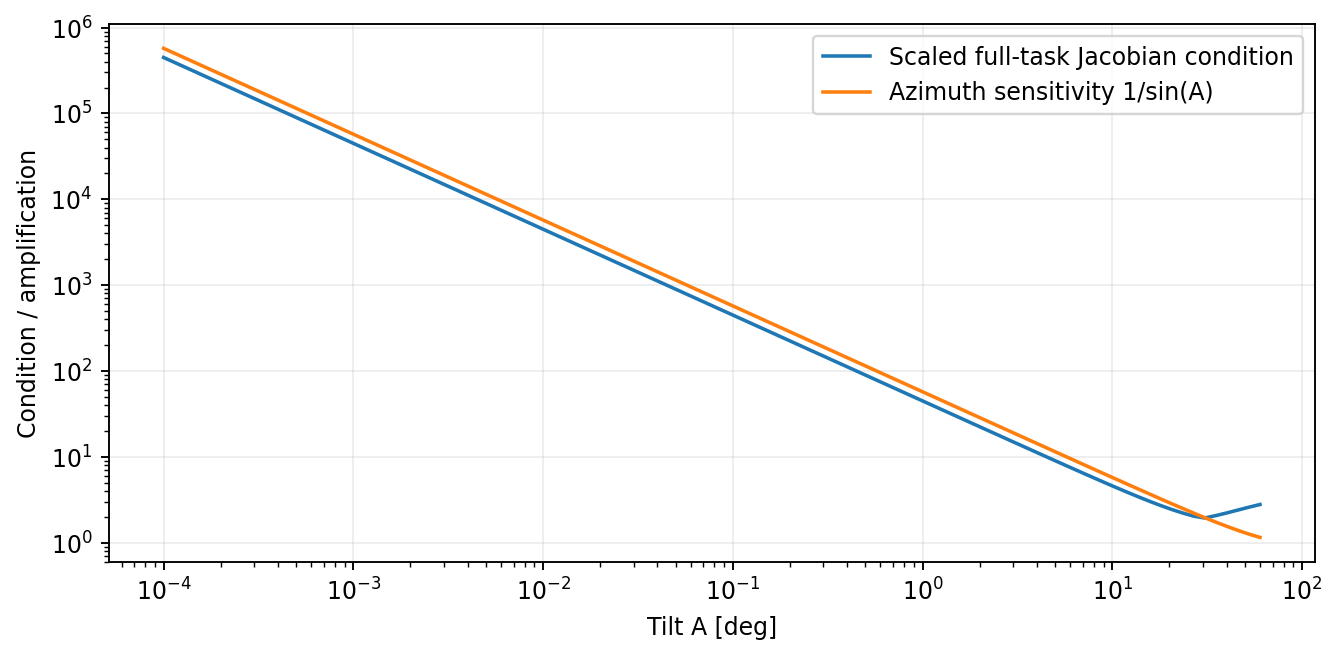
\includegraphics[width=.97\linewidth,height=73mm,keepaspectratio]{figures/singularity.png}\par\small\refstepcounter{figure}\textbf{Figure \thefigure.} Task-Jacobian conditioning and azimuth amplification near zero tilt.\end{center}

\clearpage

\section{Sensor errors, rotary representation and experimental design}

\subsection{Temperature drift and reversal play}

A fitted temperature-to-displacement map reduces pooled displacement RMS from 10.414 to 0.410 micrometres on the standalone thermal holdout. A separately identified play width of 23.993 micrometres reduces reversal-error RMS from 11.947 to 0.399. Temperature compensation uses an observed environmental state; play compensation requires the preceding direction and drive state.

\par{\small\textit{Implementation}\quad \file{remedies.py}\enspace /\enspace \file{experiments.py}}\par

\begin{center}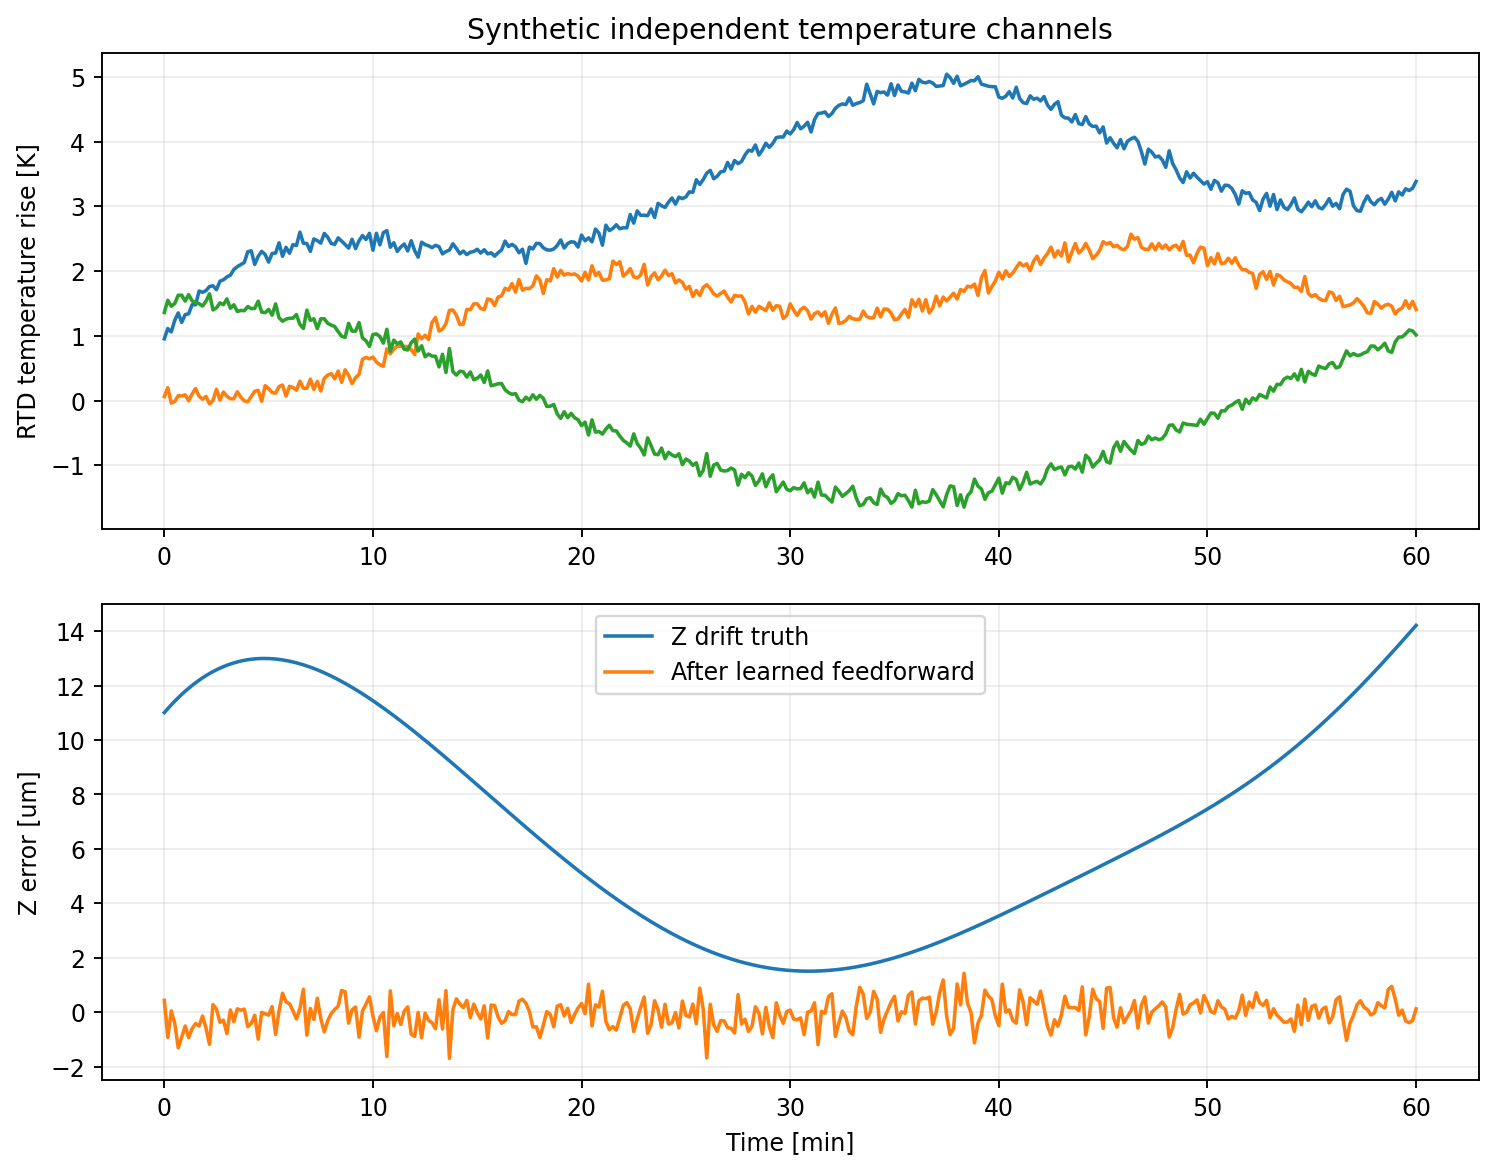
\includegraphics[width=.97\linewidth,height=73mm,keepaspectratio]{figures/thermal.png}\par\small\refstepcounter{figure}\textbf{Figure \thefigure.} Independent heating-cycle measurements and residual displacement.\end{center}

\begin{center}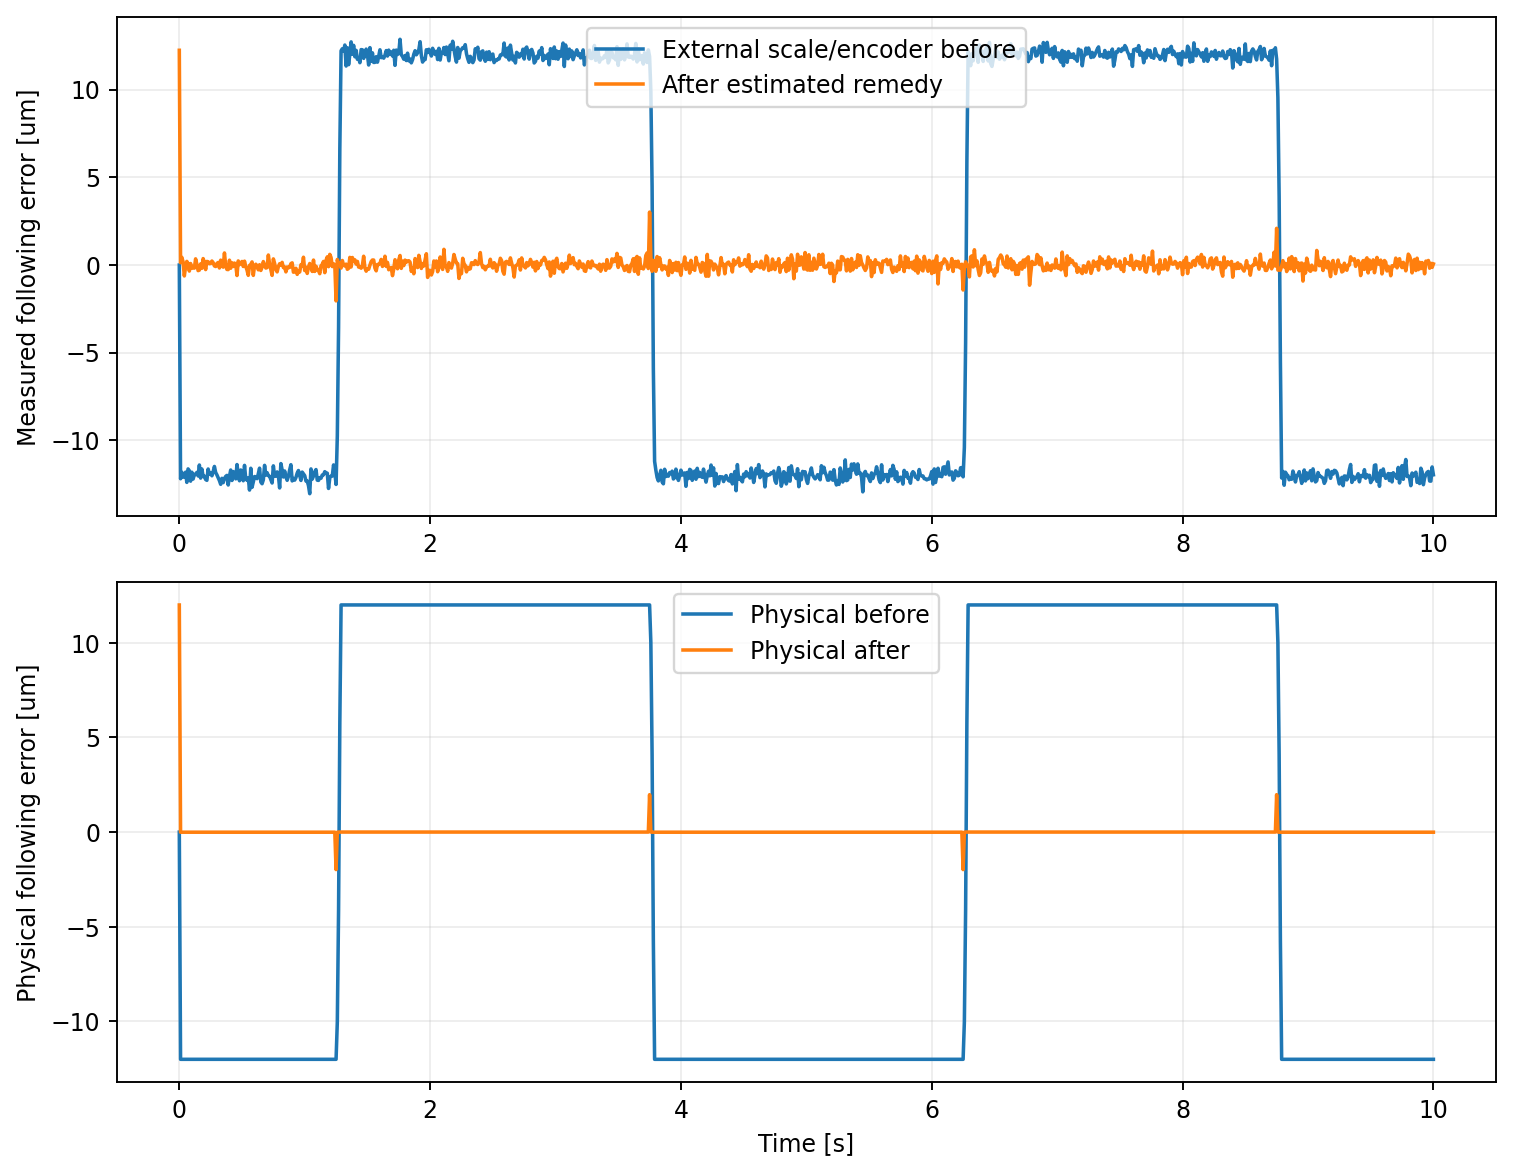
\includegraphics[width=.97\linewidth,height=73mm,keepaspectratio]{figures/backlash.png}\par\small\refstepcounter{figure}\textbf{Figure \thefigure.} External scale error before and after inverse play compensation.\end{center}

\clearpage

\subsection{Lag, offset metrology and missing channels}

For the isolated first-order drive, the identified time constant is 20.001 ms; feedforward reduces physical RMS from 1074.46 to 0.041 micrometres. For Abbe error, $e\simeq h\theta$: independent angle measurement reduces residual RMS from 2.910 to 0.205 micrometres. Median fusion reduces single-channel corruption RMS from 5.730 to 0.375 micrometres; simultaneous common-mode bias would survive that vote.

\par{\small\textit{Implementation}\quad \file{remedies.py}\enspace /\enspace \file{experiments.py}}\par

\begin{center}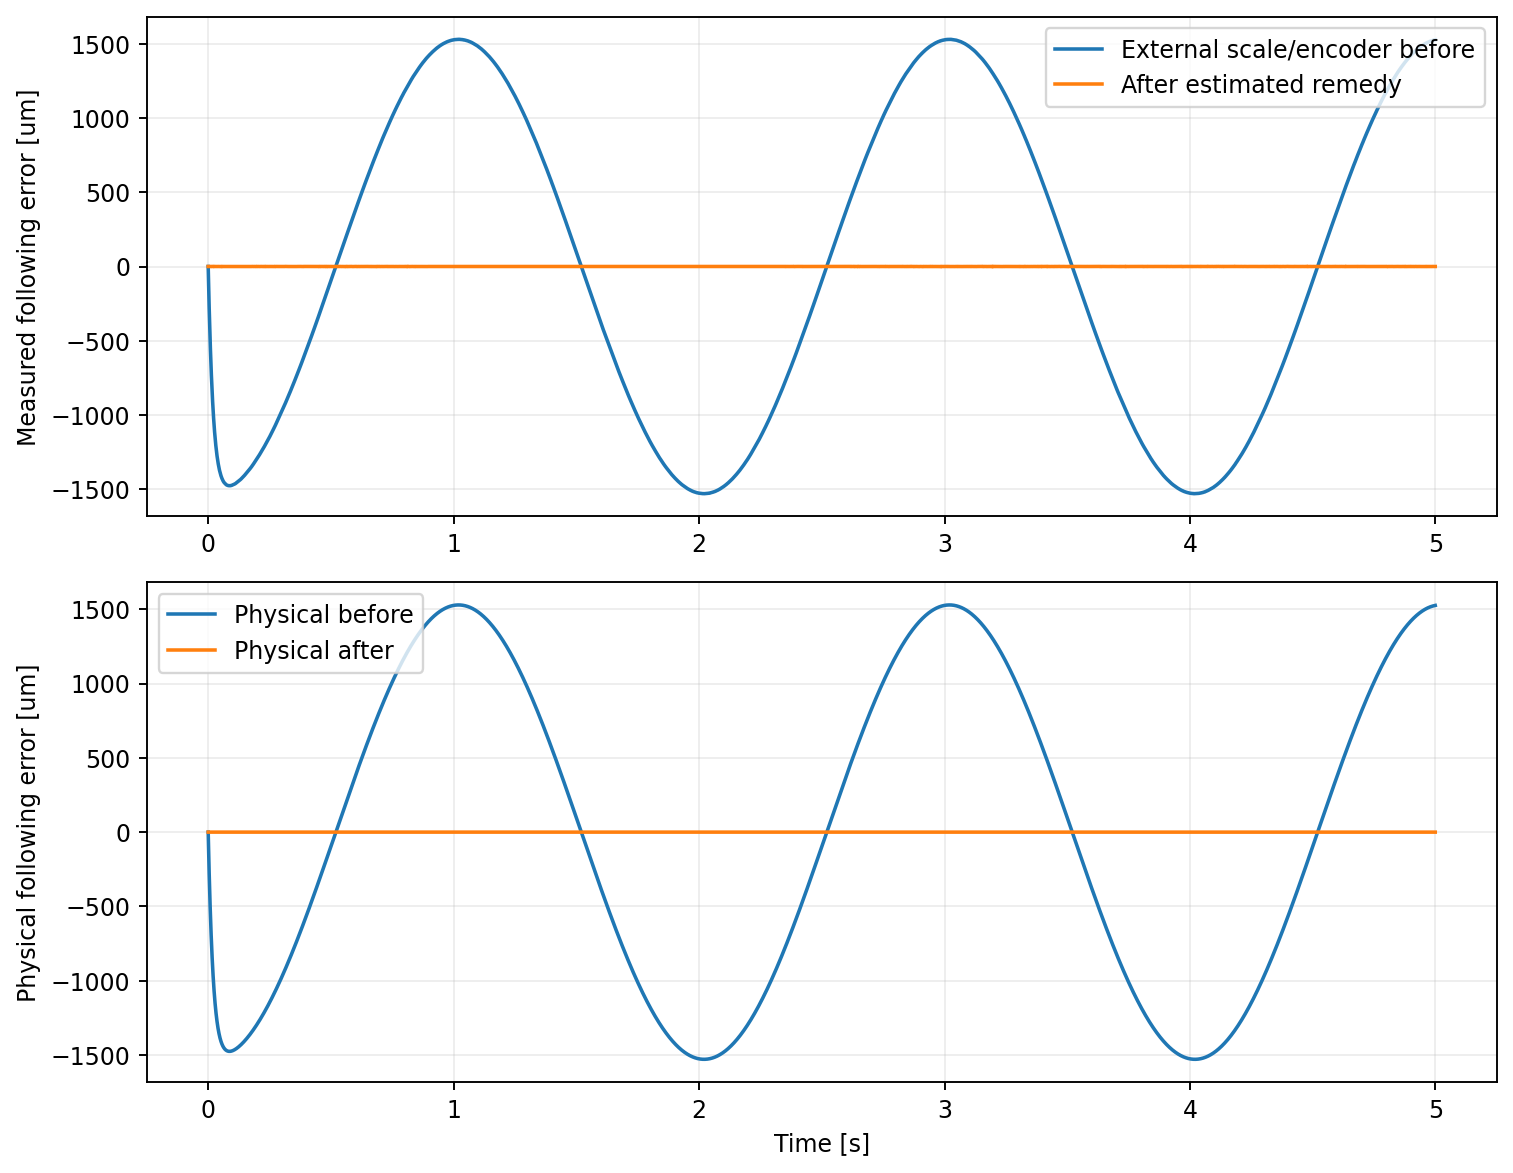
\includegraphics[width=.97\linewidth,height=47mm,keepaspectratio]{figures/servo.png}\par\small\refstepcounter{figure}\textbf{Figure \thefigure.} Sensor noise remains visible after cancellation of the simple plant lag.\end{center}

\begin{center}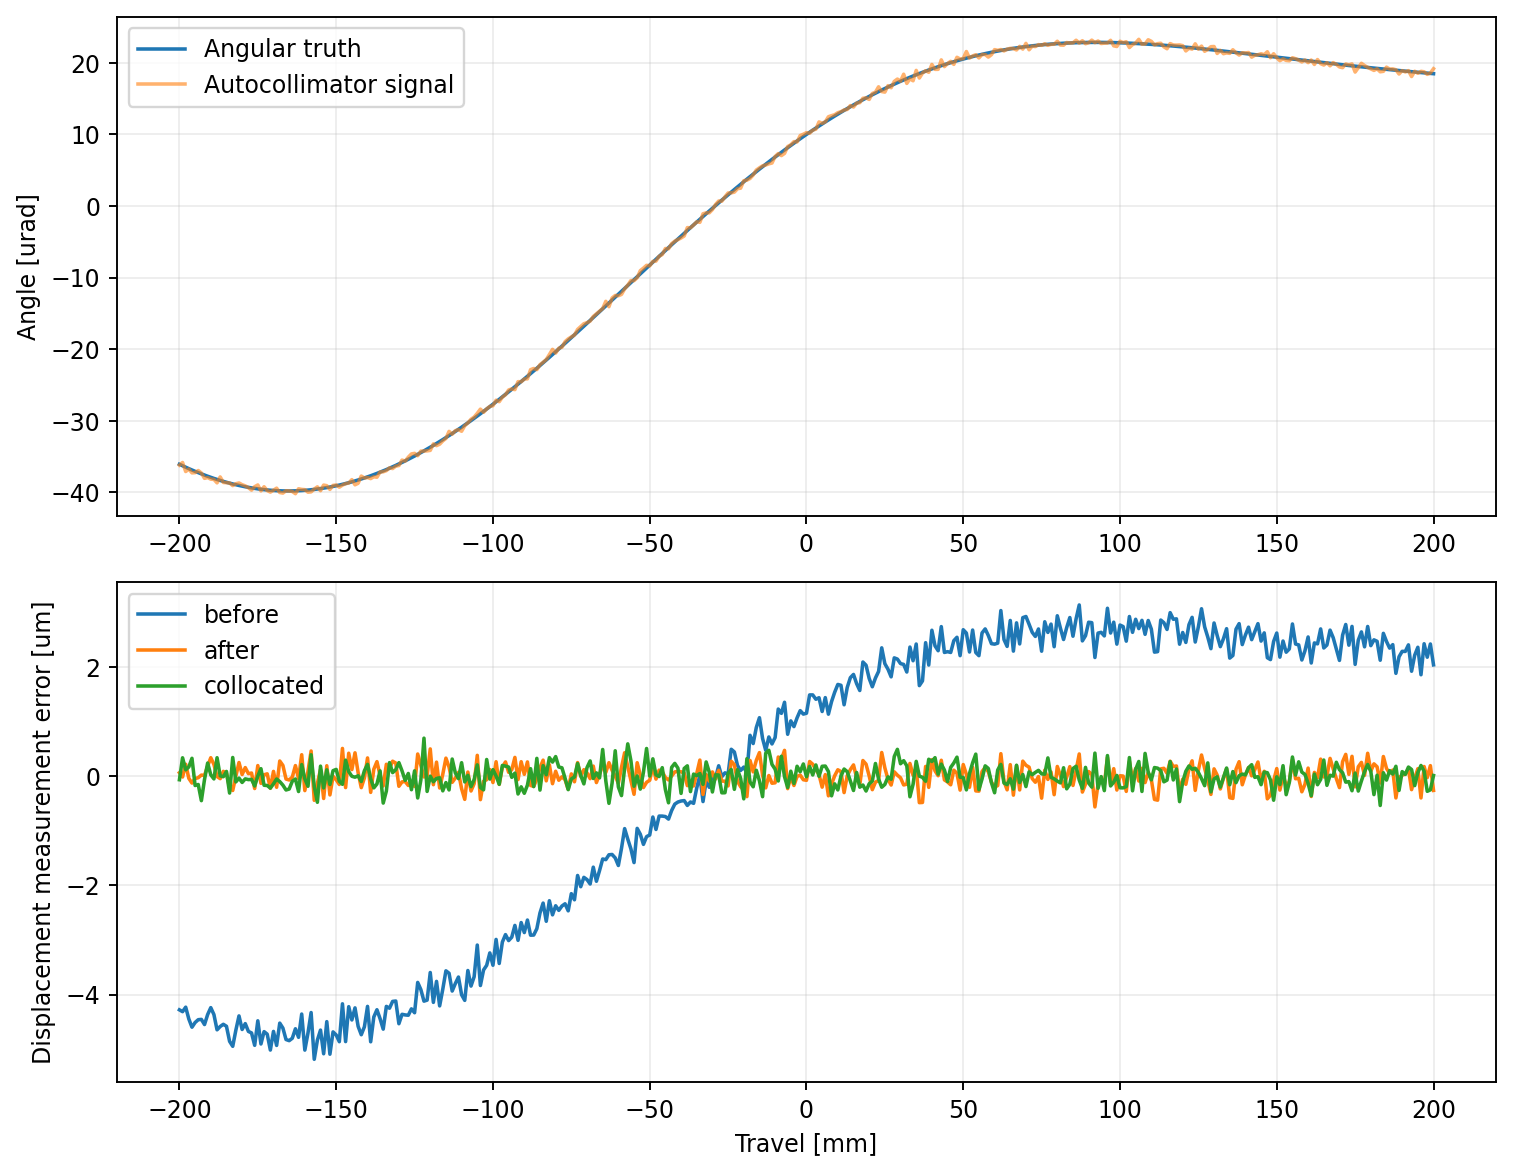
\includegraphics[width=.97\linewidth,height=47mm,keepaspectratio]{figures/abbe.png}\par\small\refstepcounter{figure}\textbf{Figure \thefigure.} Effect of angular measurement and sensor offset on linear readout.\end{center}

\begin{center}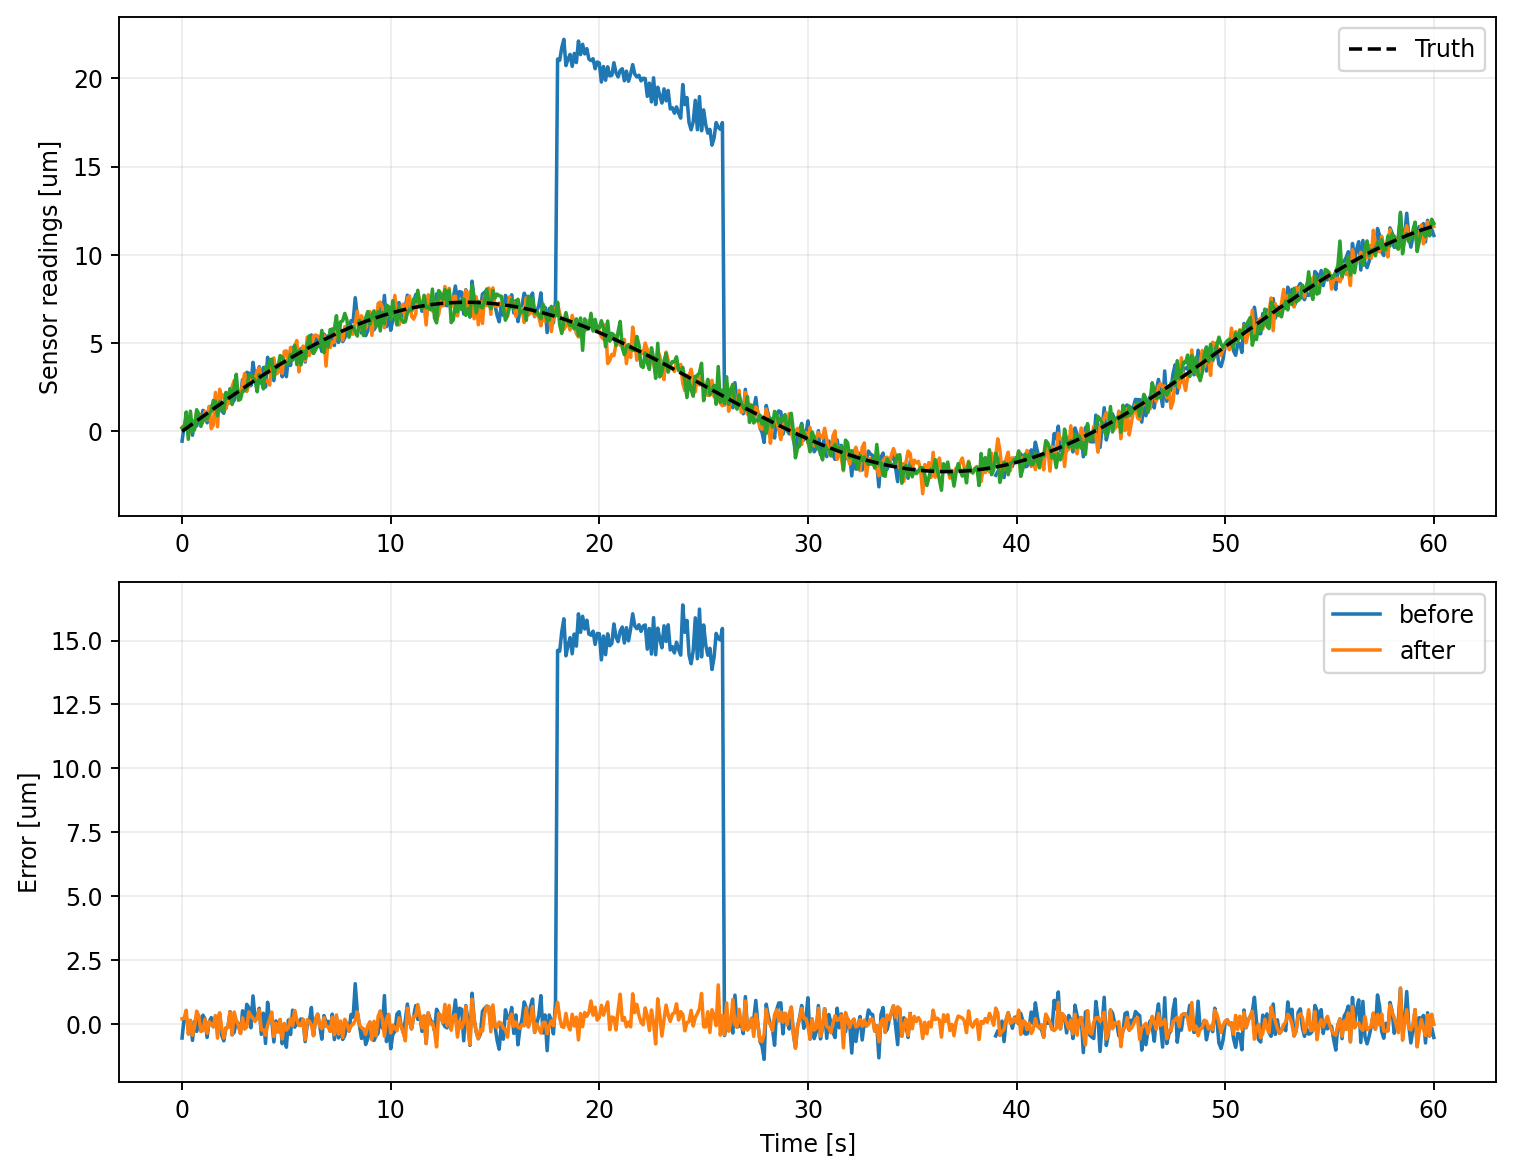
\includegraphics[width=.97\linewidth,height=47mm,keepaspectratio]{figures/sensor_faults.png}\par\small\refstepcounter{figure}\textbf{Figure \thefigure.} Three channels, a corrupted interval and a missing interval.\end{center}

\clearpage

\subsection{Extrapolating the rotating table}

The earlier independent-plant study calibrates cubic and periodic representations on the same 60 poses. The independent frame calculation then evaluates a held-out trajectory. Three-turn TCP RMS is 1878.680 micrometres with an unwrapped cubic and 1.561 with the periodic map on this example. Table 1 earlier in this report averages a different, broader protocol.

\par{\small\textit{Implementation}\quad \file{periodic_model.py}\enspace /\enspace \file{independent_plant.py}\enspace /\enspace \file{research_experiments.py}}\par

\begin{center}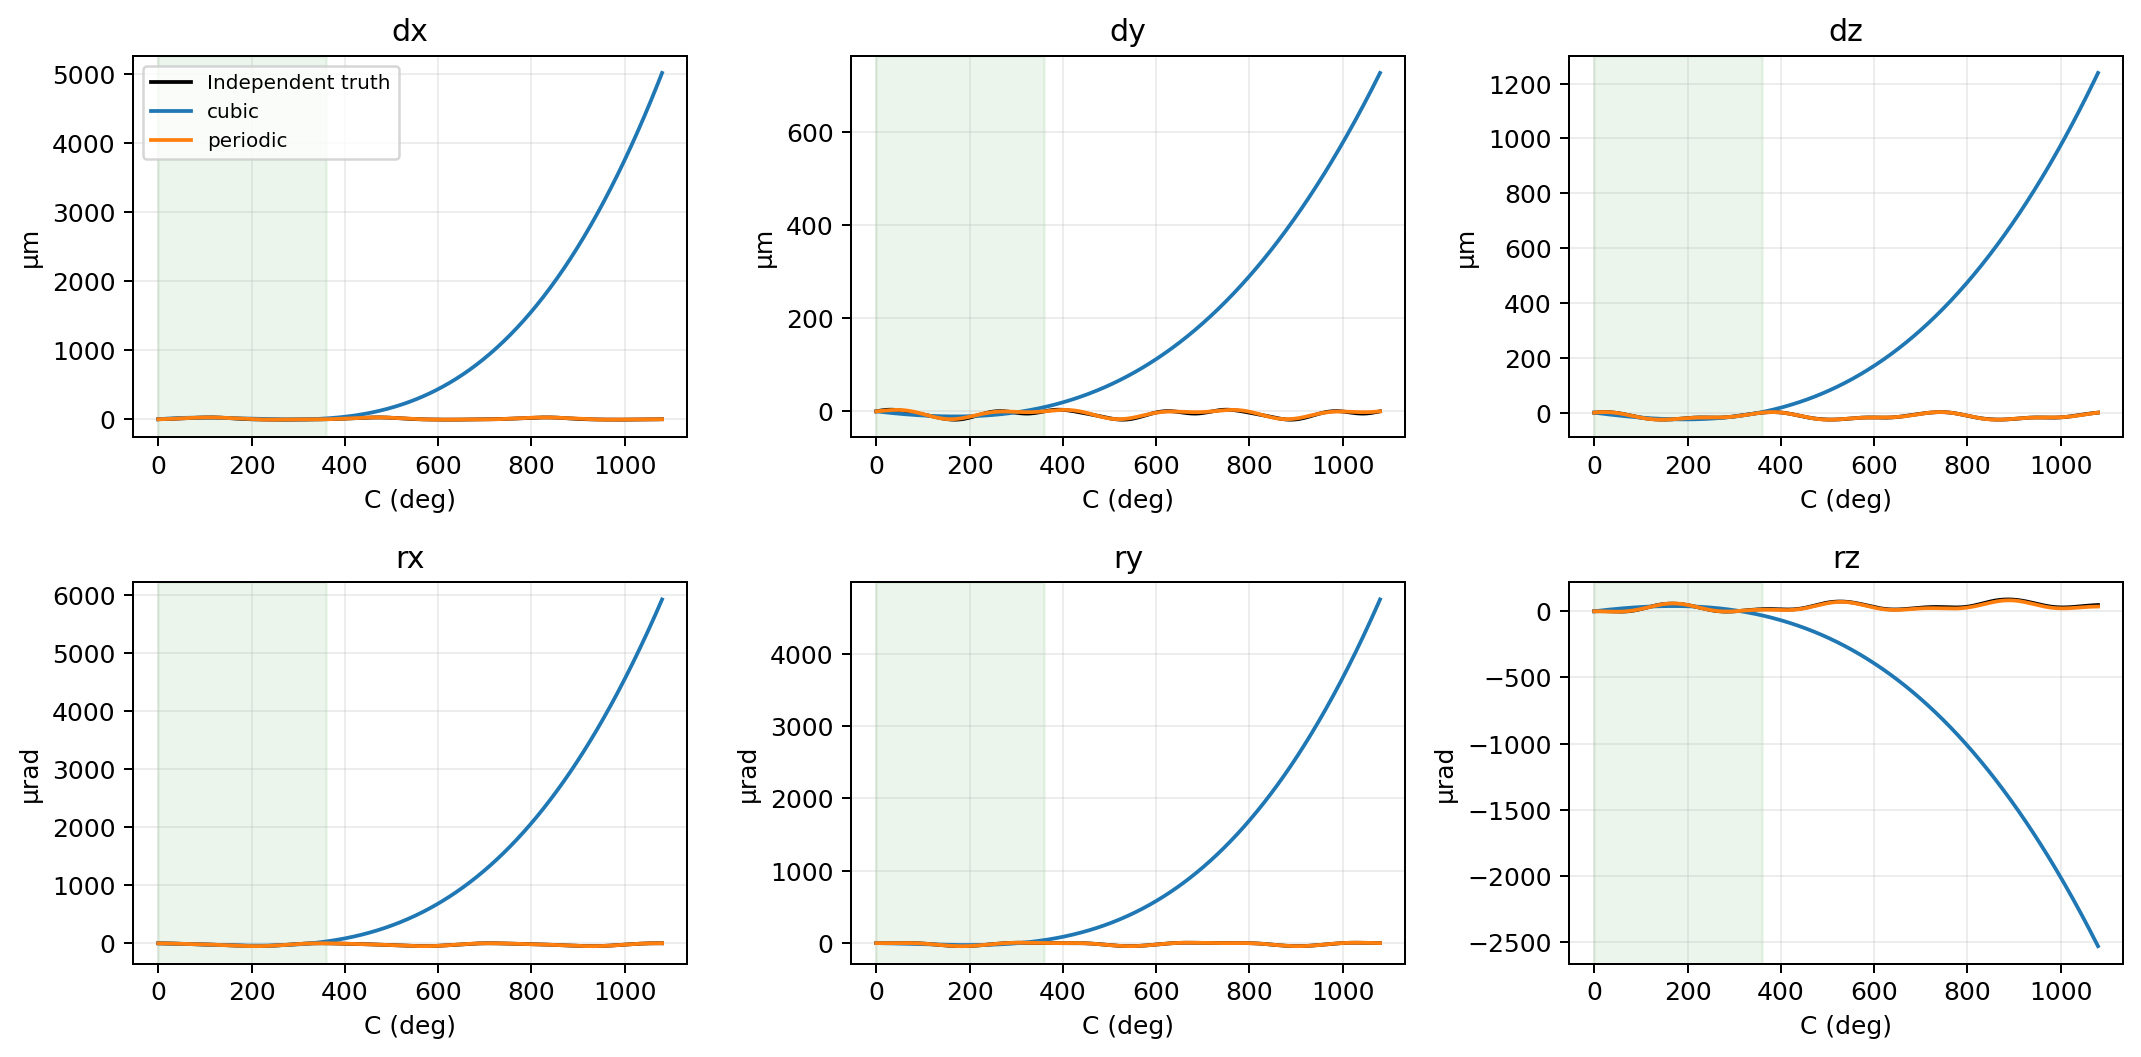
\includegraphics[width=.97\linewidth,height=73mm,keepaspectratio]{figures/research_periodic_maps.png}\par\small\refstepcounter{figure}\textbf{Figure \thefigure.} Fitted rotary channels within and beyond the training revolution.\end{center}

\begin{center}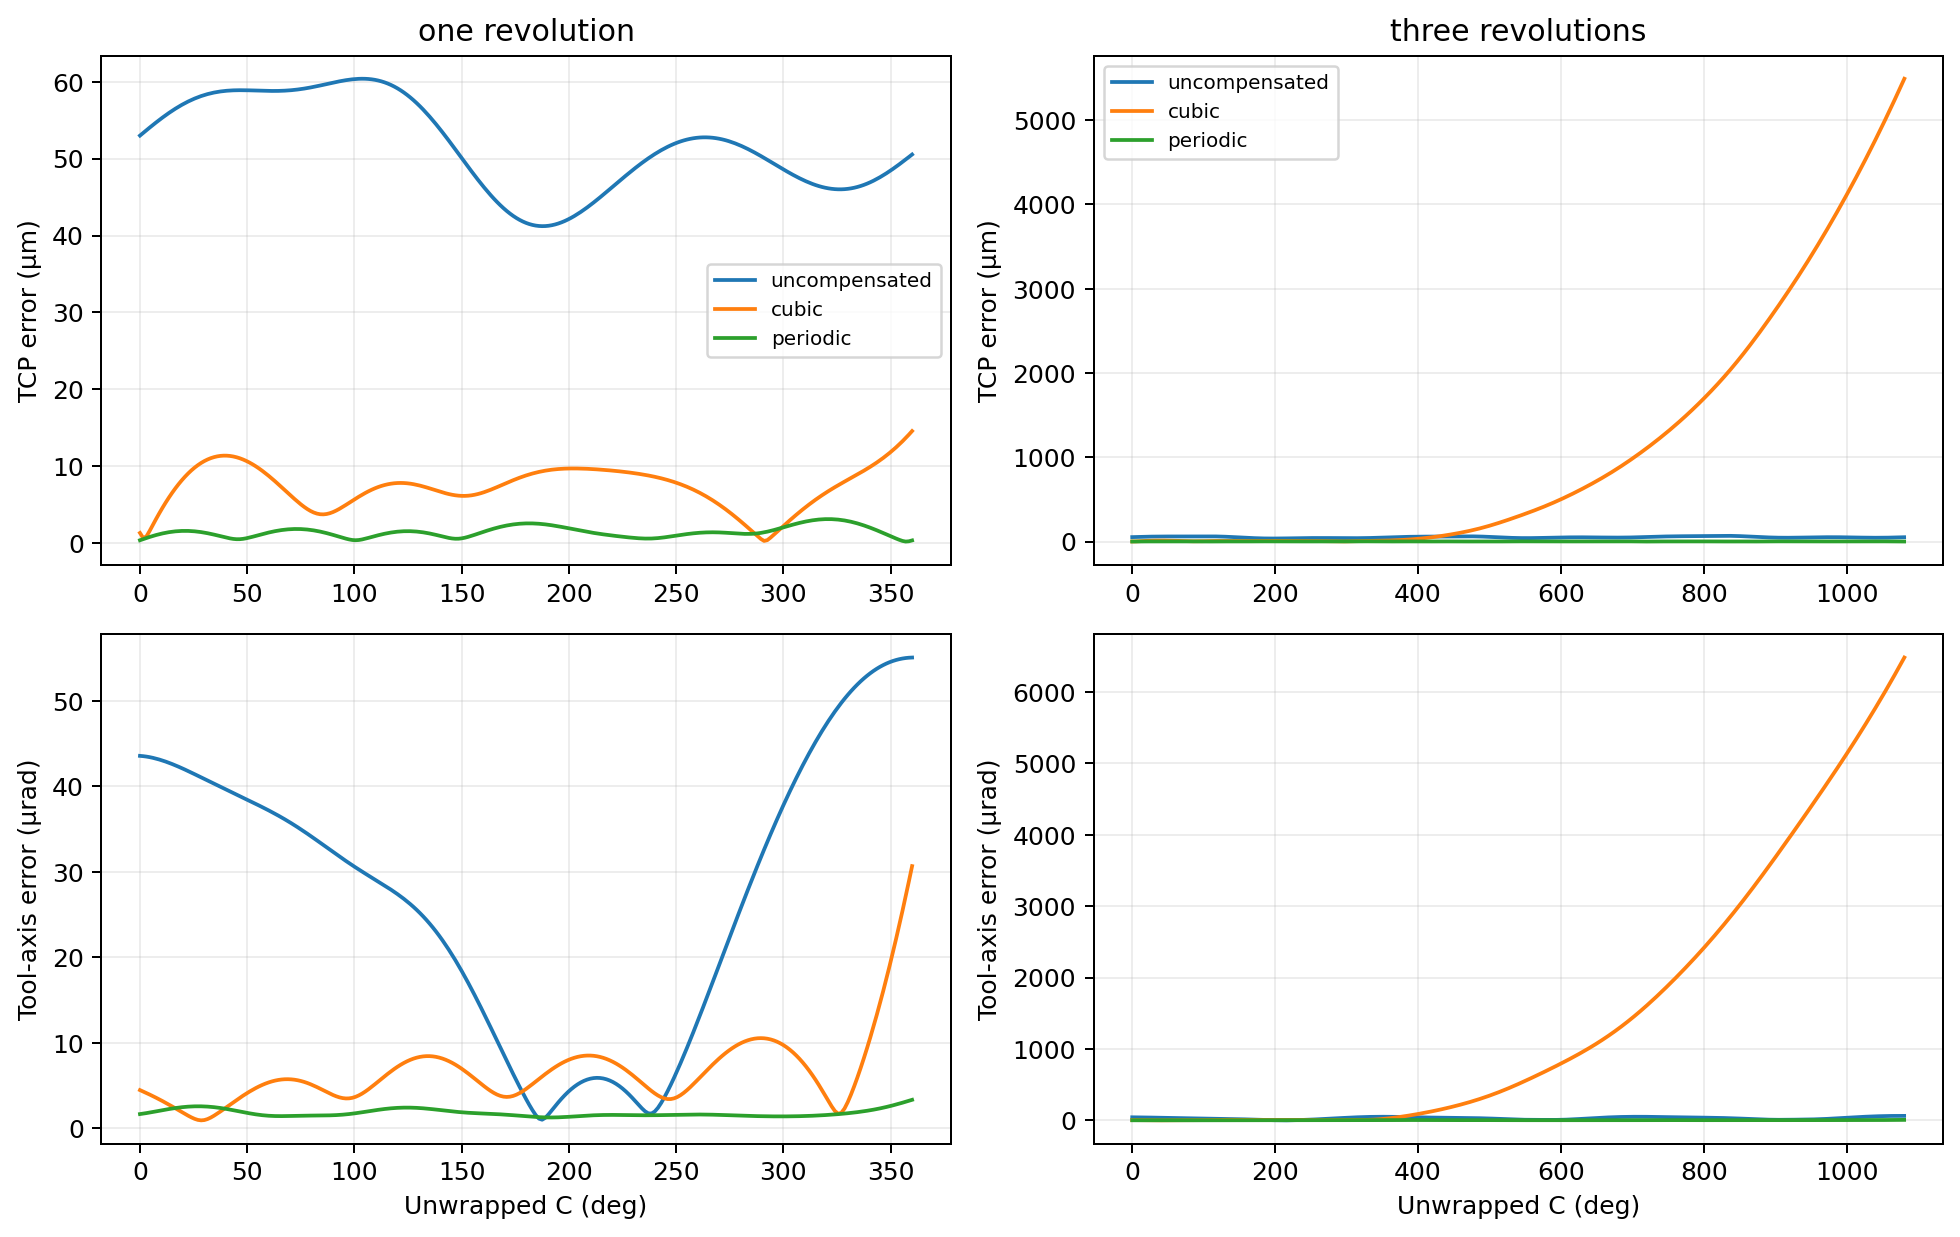
\includegraphics[width=.97\linewidth,height=73mm,keepaspectratio]{figures/research_generalization.png}\par\small\refstepcounter{figure}\textbf{Figure \thefigure.} Static TCP tracking over one and three revolutions.\end{center}

\clearpage

\subsection{Choosing calibration poses}

D-optimal selection adds the pose that most increases the log determinant of the information matrix. Space-filling selection spreads observations over normalized tilt, azimuth, height and radius. The early 24-trial design study holds auxiliary calibration fixed. Its error bars describe repeated measurements on that setup. The right-hand noise prediction explains why adding readings has a diminishing return when geometric mismatch remains.

\par{\small\textit{Implementation}\quad \file{periodic_model.py}\enspace /\enspace \file{research_experiments.py}}\par

\begin{center}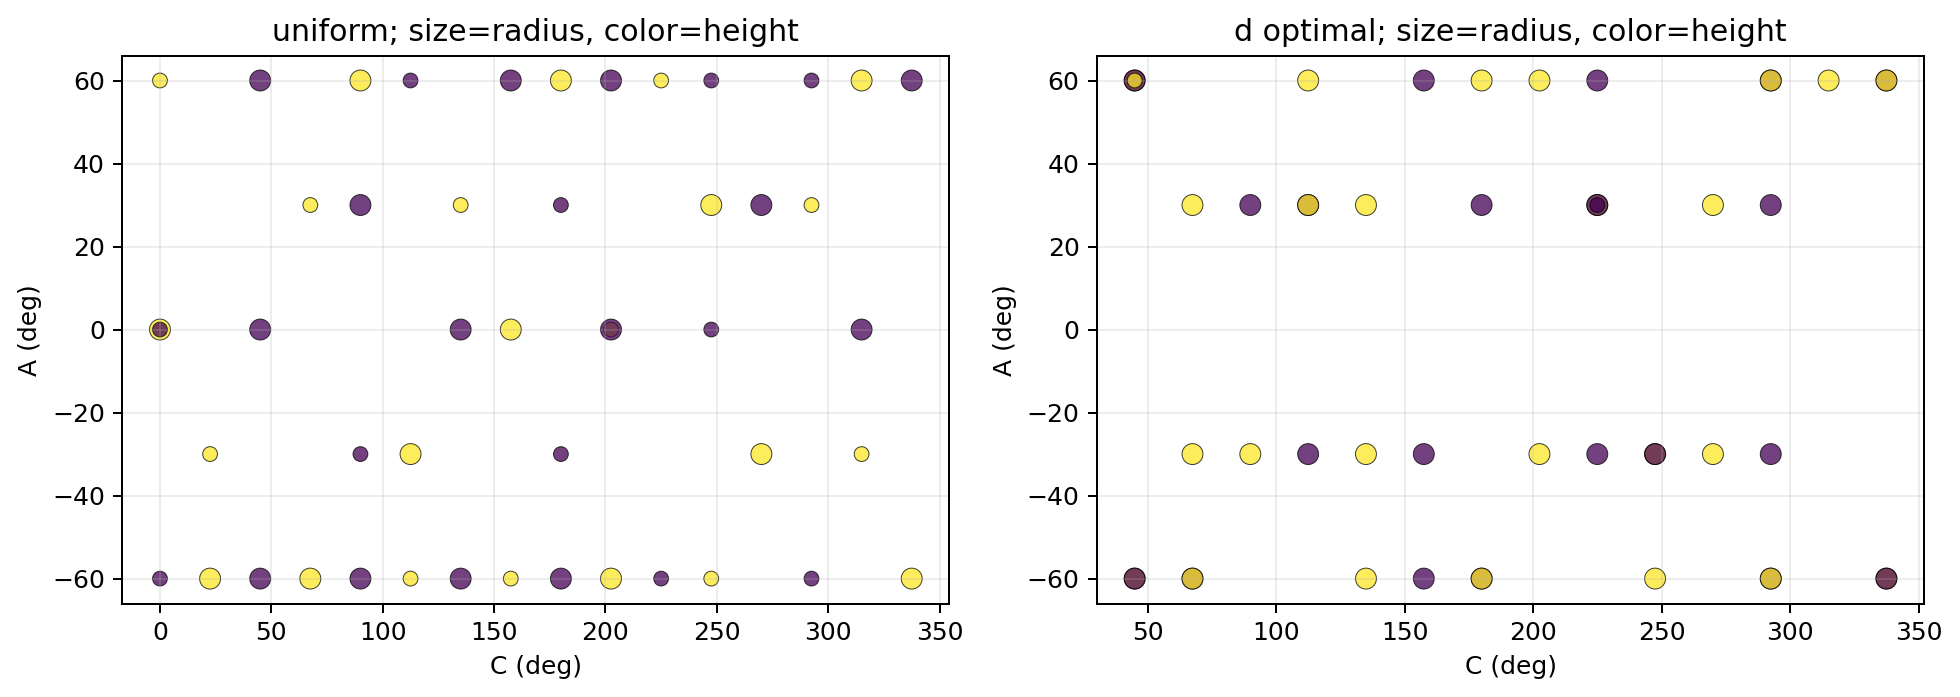
\includegraphics[width=.97\linewidth,height=73mm,keepaspectratio]{figures/research_pose_selection.png}\par\small\refstepcounter{figure}\textbf{Figure \thefigure.} Two 48-pose selections from the same candidate set.\end{center}

\begin{center}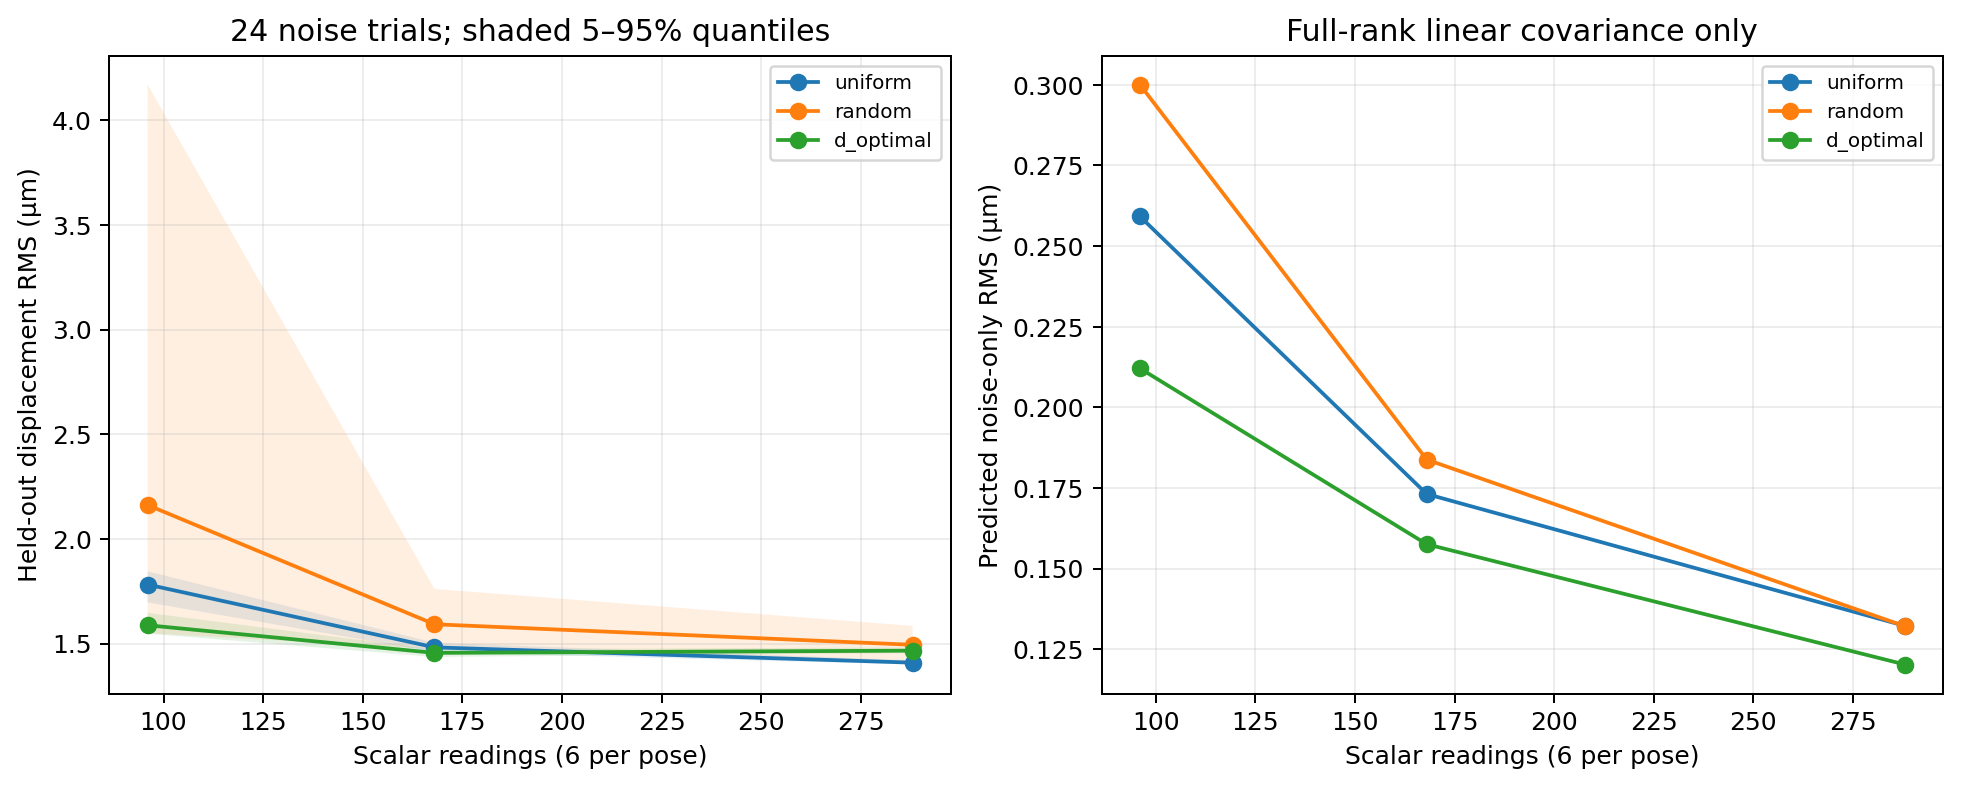
\includegraphics[width=.97\linewidth,height=73mm,keepaspectratio]{figures/research_design.png}\par\small\refstepcounter{figure}\textbf{Figure \thefigure.} Held-out displacement RMS and the conditional noise contribution.\end{center}

\clearpage

\subsection{How to spend a scalar-reading budget}

At fixed zero tilt, the 18 A-axis map columns vanish, leaving rank 25/43. With varied tilt, position-only observations already reach 43/43. Buying three more angle readings per pose then trades independent directions against workspace coverage. At a budget of 288 scalar readings, position-only sampling permits 96 poses and yields 0.107 micrometres noise RMS; six-channel sampling permits 48 poses and yields 0.118 in the task I-optimal comparison.

\par{\small\textit{Implementation}\quad \file{publication_studies.py}\enspace /\enspace \file{research_dashboard.py}}\par

\begin{center}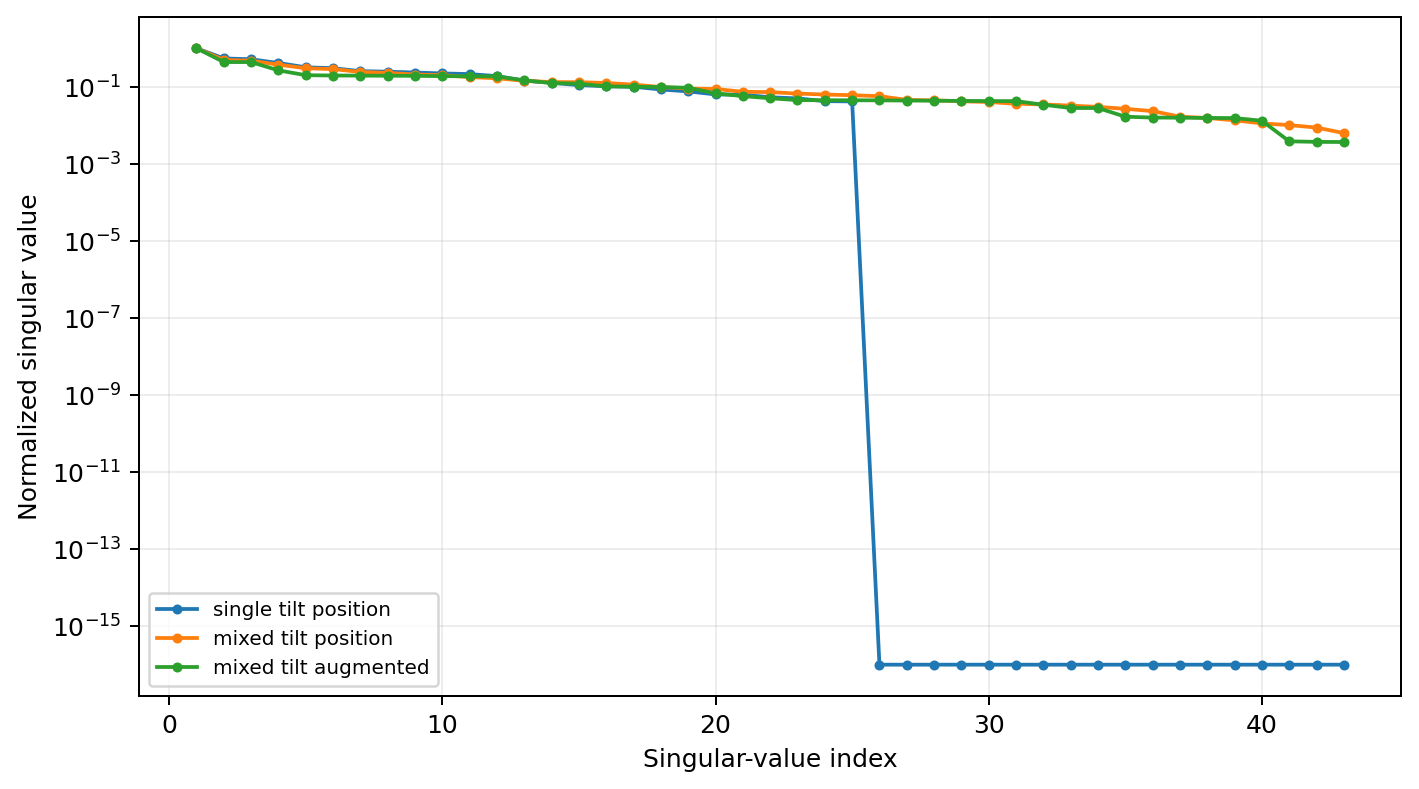
\includegraphics[width=.97\linewidth,height=73mm,keepaspectratio]{figures/research_observability.png}\par\small\refstepcounter{figure}\textbf{Figure \thefigure.} Singular spectra under tilt restriction and different observation channels.\end{center}

\begin{center}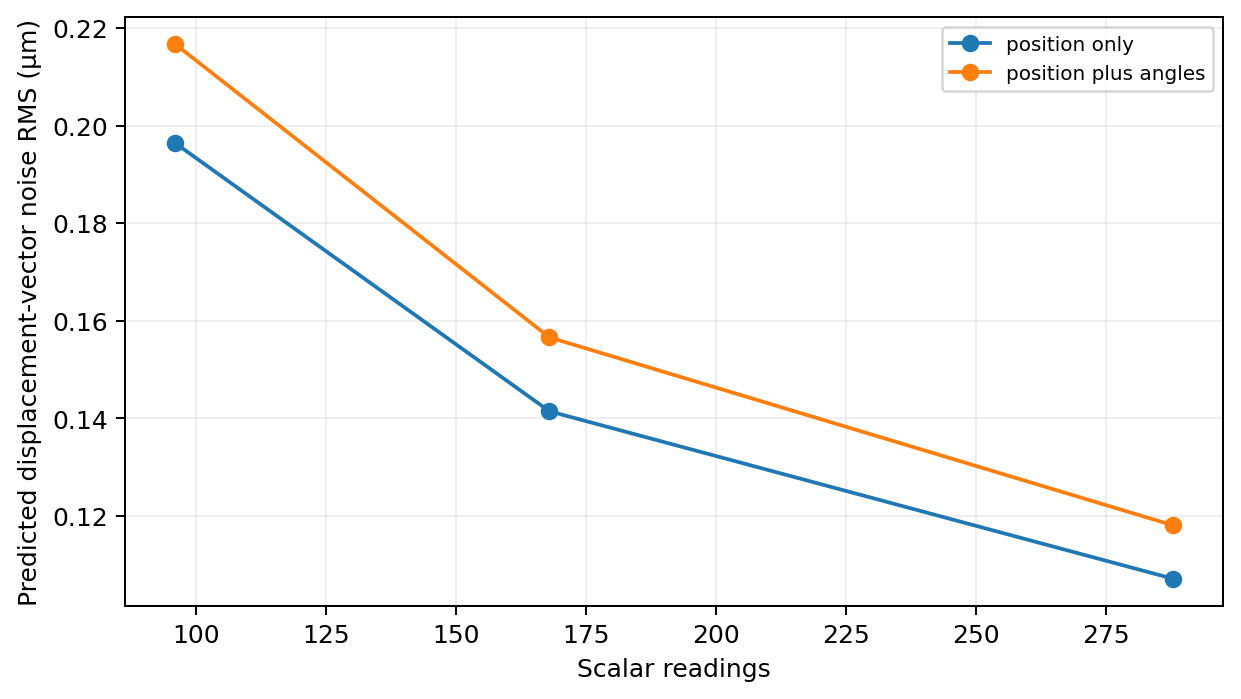
\includegraphics[width=.97\linewidth,height=73mm,keepaspectratio]{figures/publication_sensor_budget.png}\par\small\refstepcounter{figure}\textbf{Figure \thefigure.} Equal-reading comparison across three budgets.\end{center}

\clearpage

\subsection{Separating design noise from omitted geometry}

In the expanded study, seed, configuration, design, omitted-error amplitude and noise draw are varied. With 48 poses and unit omission amplitude, D-optimal selection gives 1.244 micrometres total RMS, including 1.228 micrometres noiseless bias. At triple amplitude the corresponding values are 3.689 and 3.683. The predicted rotary-noise component stays at 0.125 because it depends on the fitted sensitivity and sensor law.

\par{\small\textit{Implementation}\quad \file{publication_studies.py}}\par

\begin{center}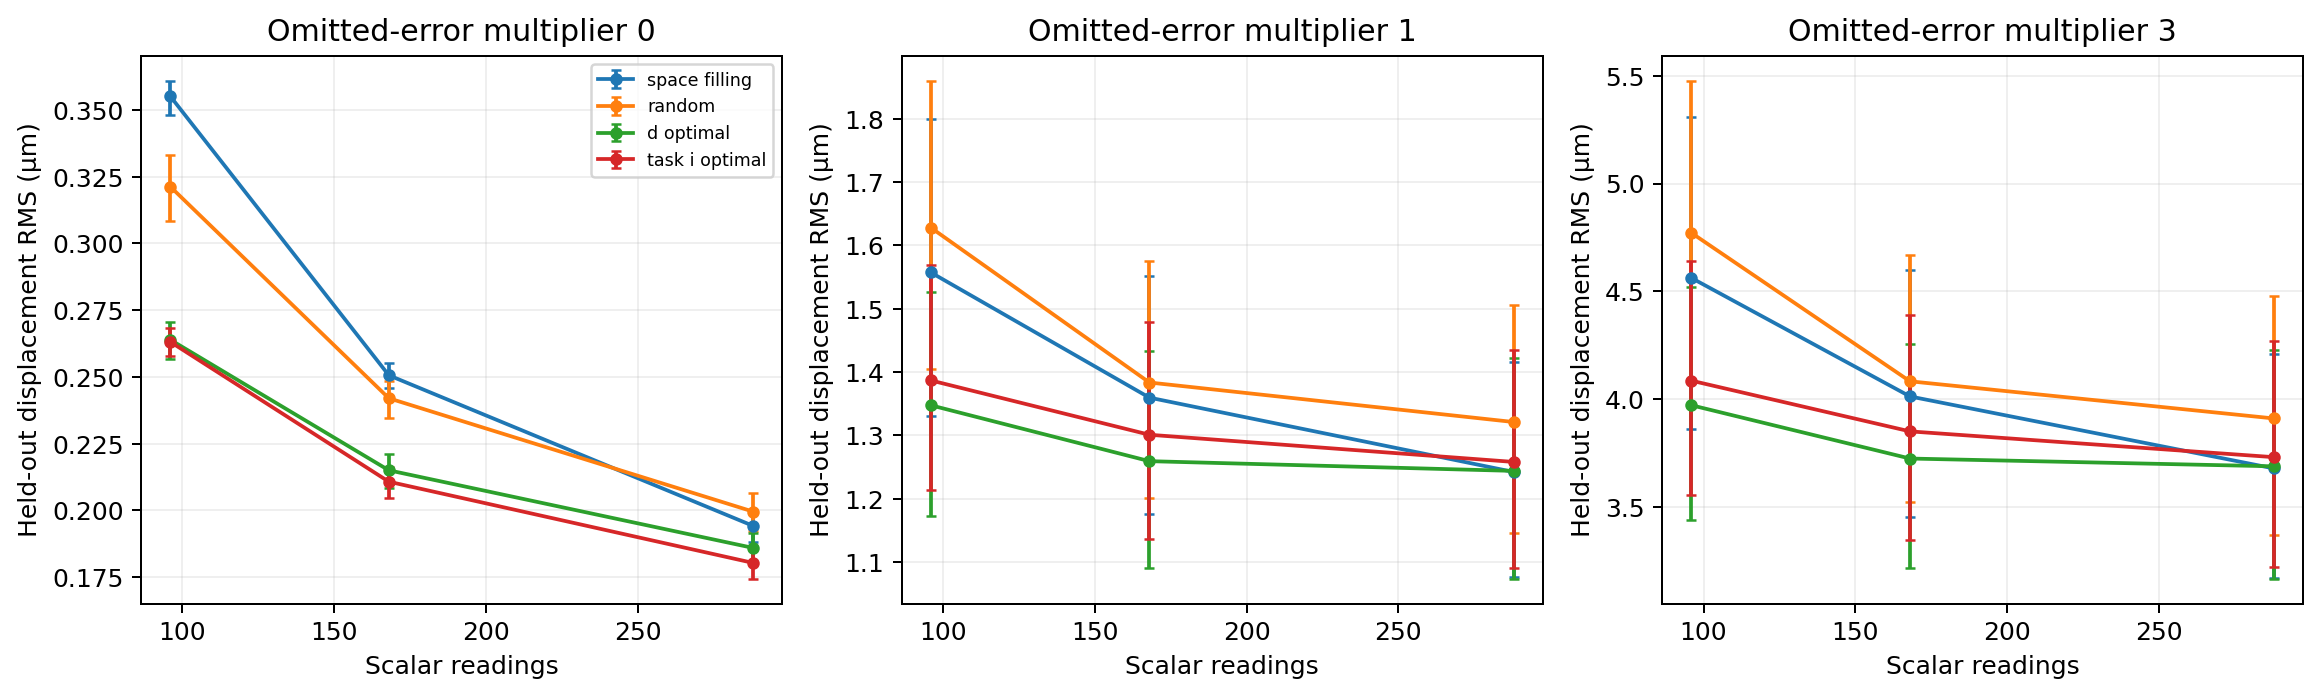
\includegraphics[width=.97\linewidth,height=73mm,keepaspectratio]{figures/publication_design_panel.png}\par\small\refstepcounter{figure}\textbf{Figure \thefigure.} Paired, equal-budget assessment across designs and truth configurations.\end{center}

\begin{center}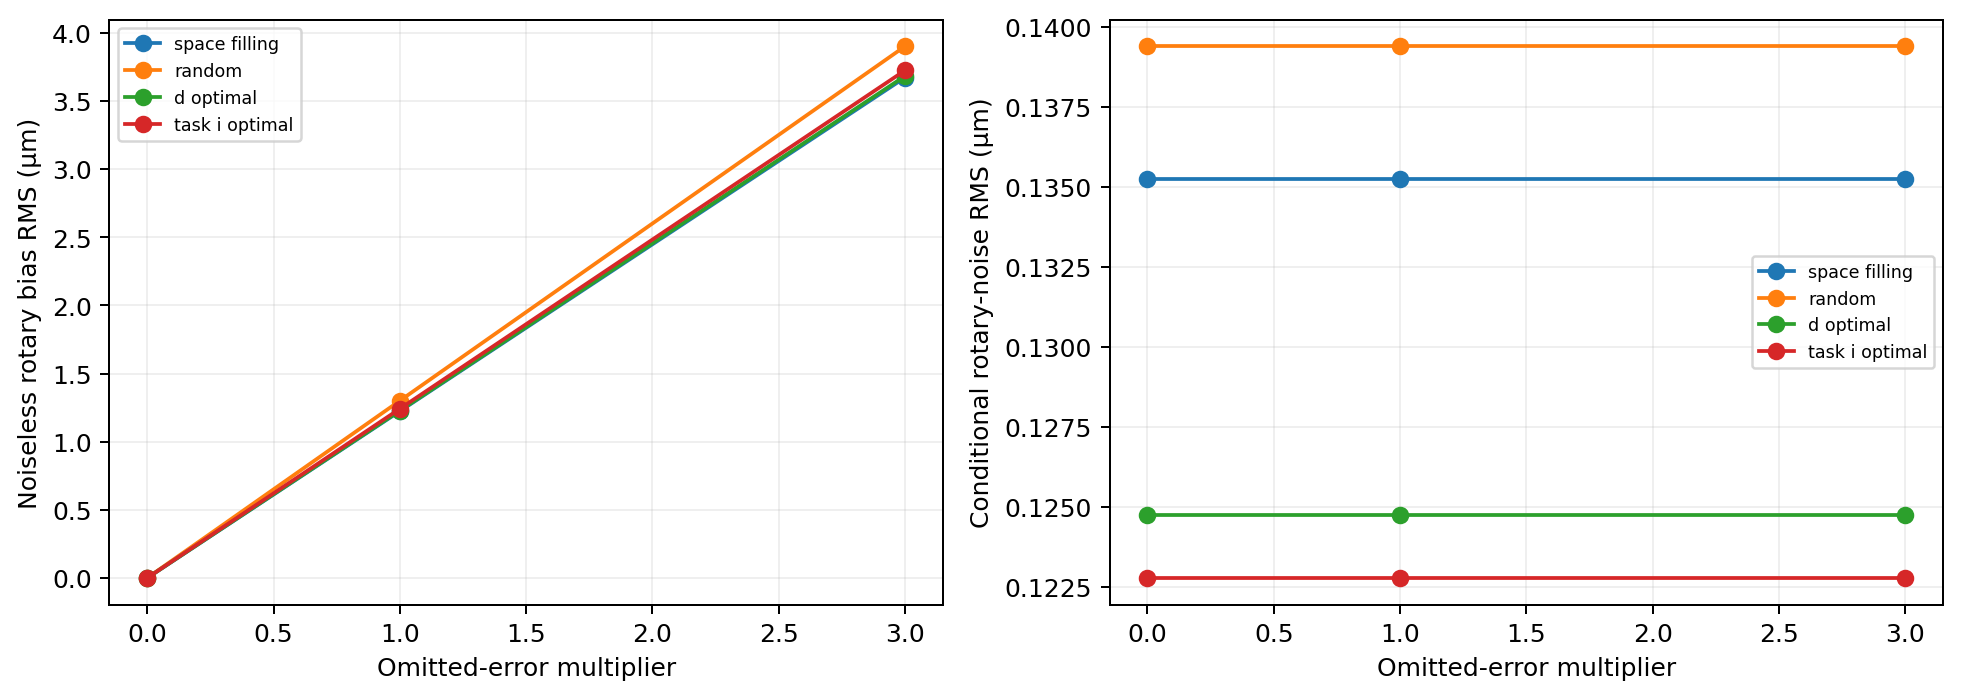
\includegraphics[width=.97\linewidth,height=73mm,keepaspectratio]{figures/publication_bias_variance.png}\par\small\refstepcounter{figure}\textbf{Figure \thefigure.} Noise-only and noiseless terms as omitted-error amplitude increases.\end{center}

\clearpage

\subsection{A fairer rotary representation comparison}

Wrapping the cubic at each revolution tests how much of the multi-turn failure is simple extrapolation. A second control matches the number of coefficients: five- and nine-knot periodic cubic splines match the two- and four-harmonic maps at 43 and 67 parameters. At 67 coefficients on localized truth, the three-turn RMS is 0.533 micrometres for Fourier and 0.597 for the spline. The model families encode different smooth shapes even at equal capacity.

\par{\small\textit{Implementation}\quad \file{publication_studies.py}\enspace /\enspace \file{journal_studies.py}}\par

\begin{center}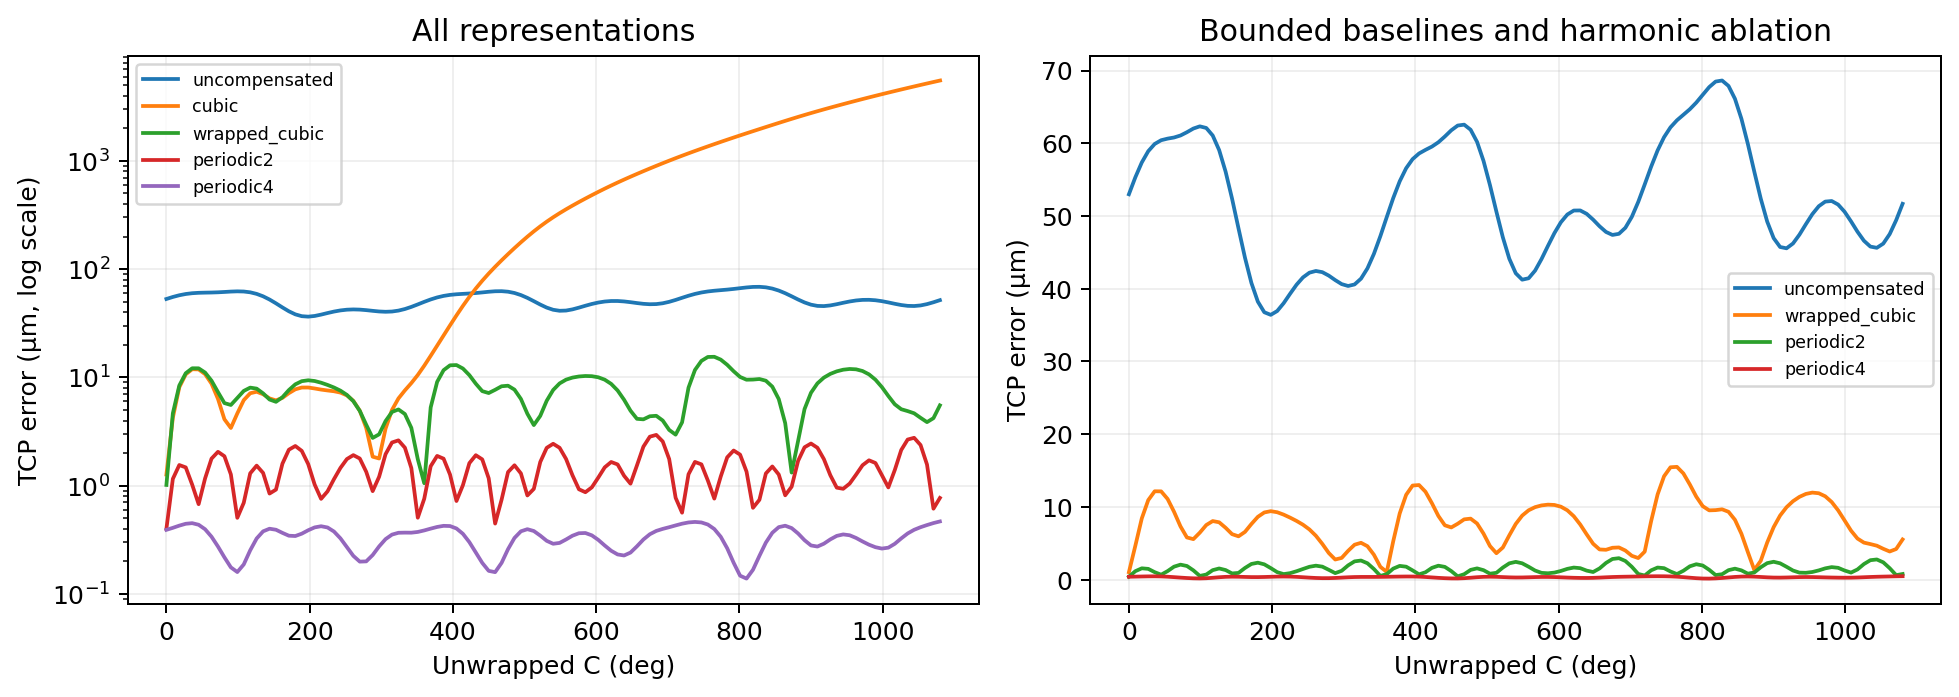
\includegraphics[width=.97\linewidth,height=73mm,keepaspectratio]{figures/publication_wrapped_baseline.png}\par\small\refstepcounter{figure}\textbf{Figure \thefigure.} Wrapped and unwrapped baselines on the same three-turn case.\end{center}

\begin{center}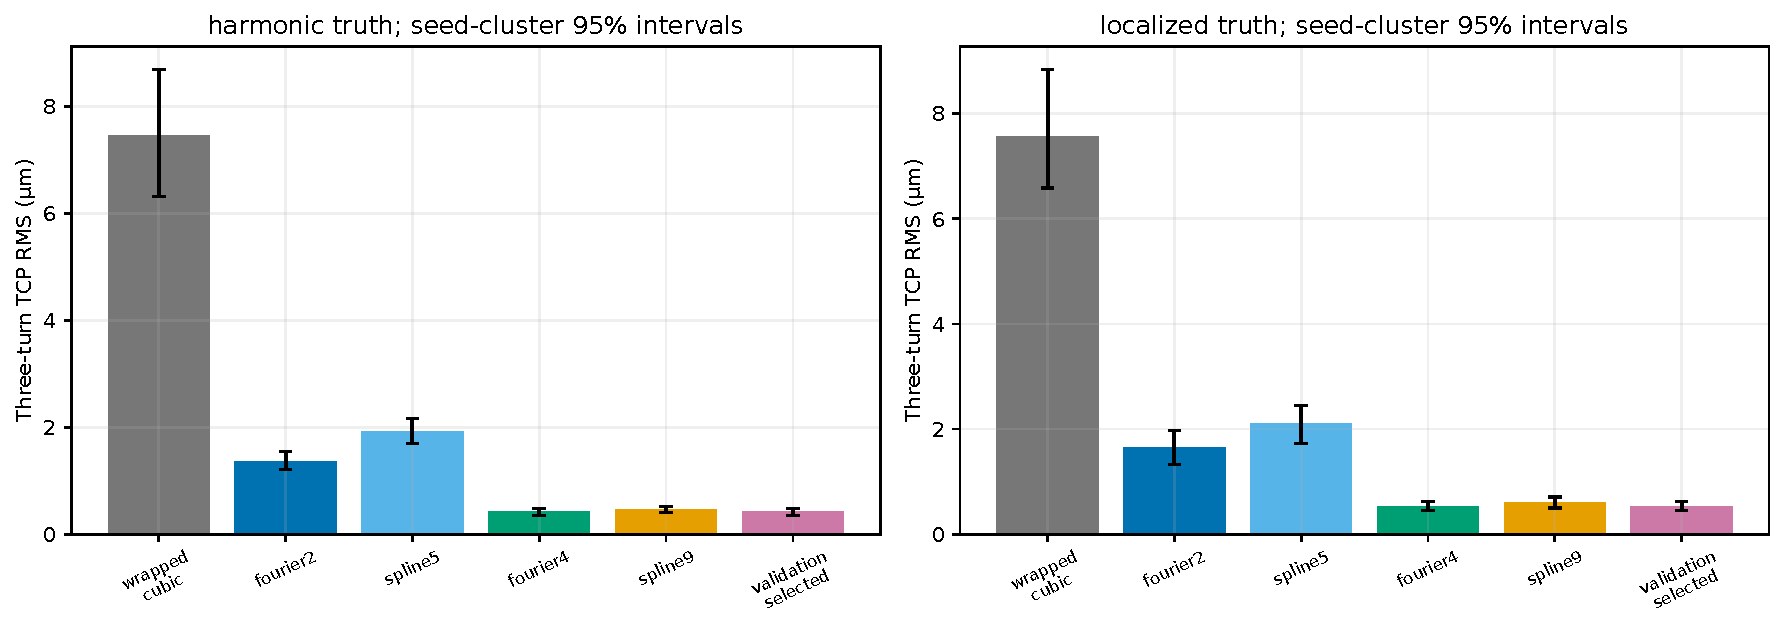
\includegraphics[width=.97\linewidth,height=73mm,keepaspectratio]{figures/journal_equal_capacity.pdf}\par\small\refstepcounter{figure}\textbf{Figure \thefigure.} Comparison under harmonic and localized truth, with seed-cluster intervals.\end{center}

\clearpage

\subsection{Selecting a map using sensor data}

Selection uses 32 disjoint six-channel validation poses. Each candidate is scored on its normalized rotary sensor residuals; the held-out TCP path is reserved for assessment. Across 36 seed/configuration pairs per family, the resulting selected models give three-turn mean RMS of 0.417 micrometres on harmonic truth and 0.533 on localized truth. A validation score can support a model choice without access to exact tool positions.

\par{\small\textit{Implementation}\quad \file{journal_models.py}\enspace /\enspace \file{journal_studies.py}}\par

\begin{center}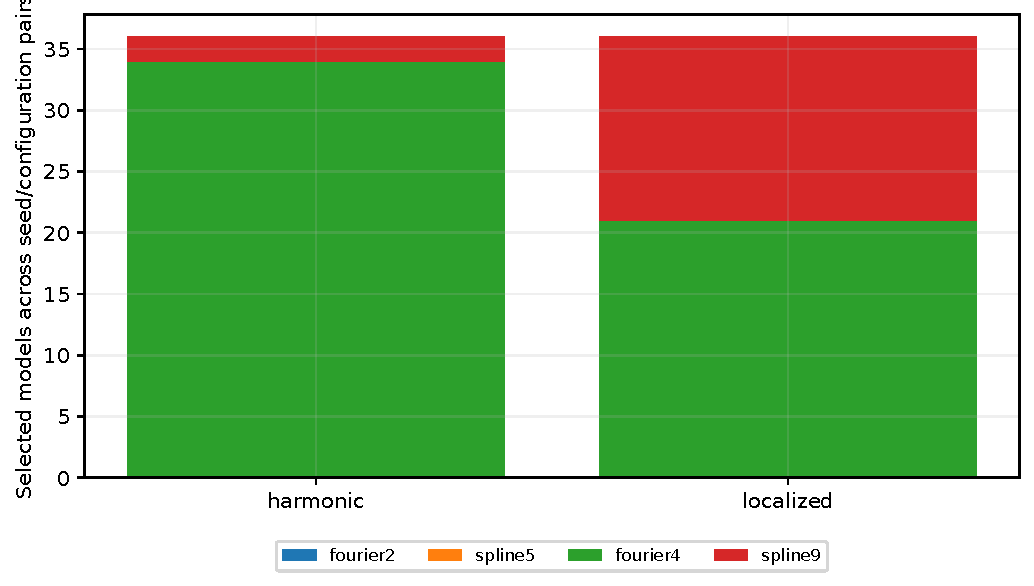
\includegraphics[width=.97\linewidth,height=73mm,keepaspectratio]{figures/journal_model_selection.pdf}\par\small\refstepcounter{figure}\textbf{Figure \thefigure.} Frequency with which each candidate wins on validation readings.\end{center}

\begin{center}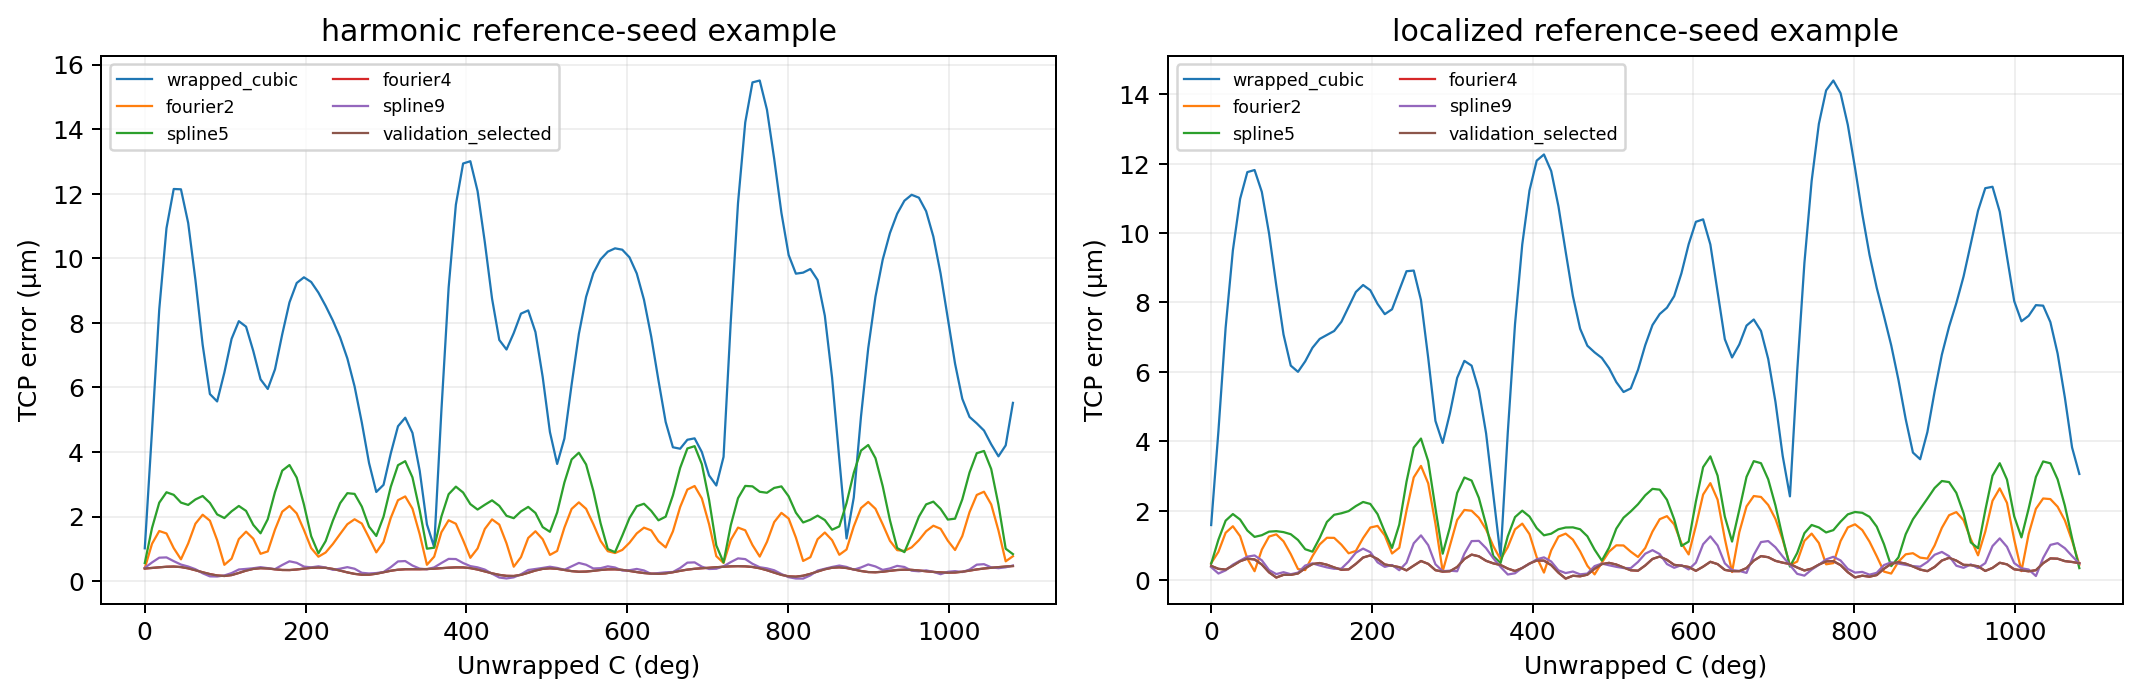
\includegraphics[width=.97\linewidth,height=73mm,keepaspectratio]{figures/journal_family_sensor_traces.png}\par\small\refstepcounter{figure}\textbf{Figure \thefigure.} Position traces on the assessment path for one reference seed.\end{center}

\clearpage

\section{Dynamic execution and independent sensing}

\subsection{Following a moving path}

The early study uses a sequential two-pole lag approximation. On its 30 s trajectory, uncompensated TCP RMS is 330.81 micrometres. Adding geometry, thermal compensation and inverse play gives 287.99; adding feedforward brings it to 44.38. In the slower 60 s case the full-remedy RMS is 29.18. These values belong to the earlier integrator. The following physical-time study uses an exact zero-order-hold (ZOH) update.

\par{\small\textit{Implementation}\quad \file{dynamic_sim.py}\enspace /\enspace \file{research_experiments.py}}\par

\begin{center}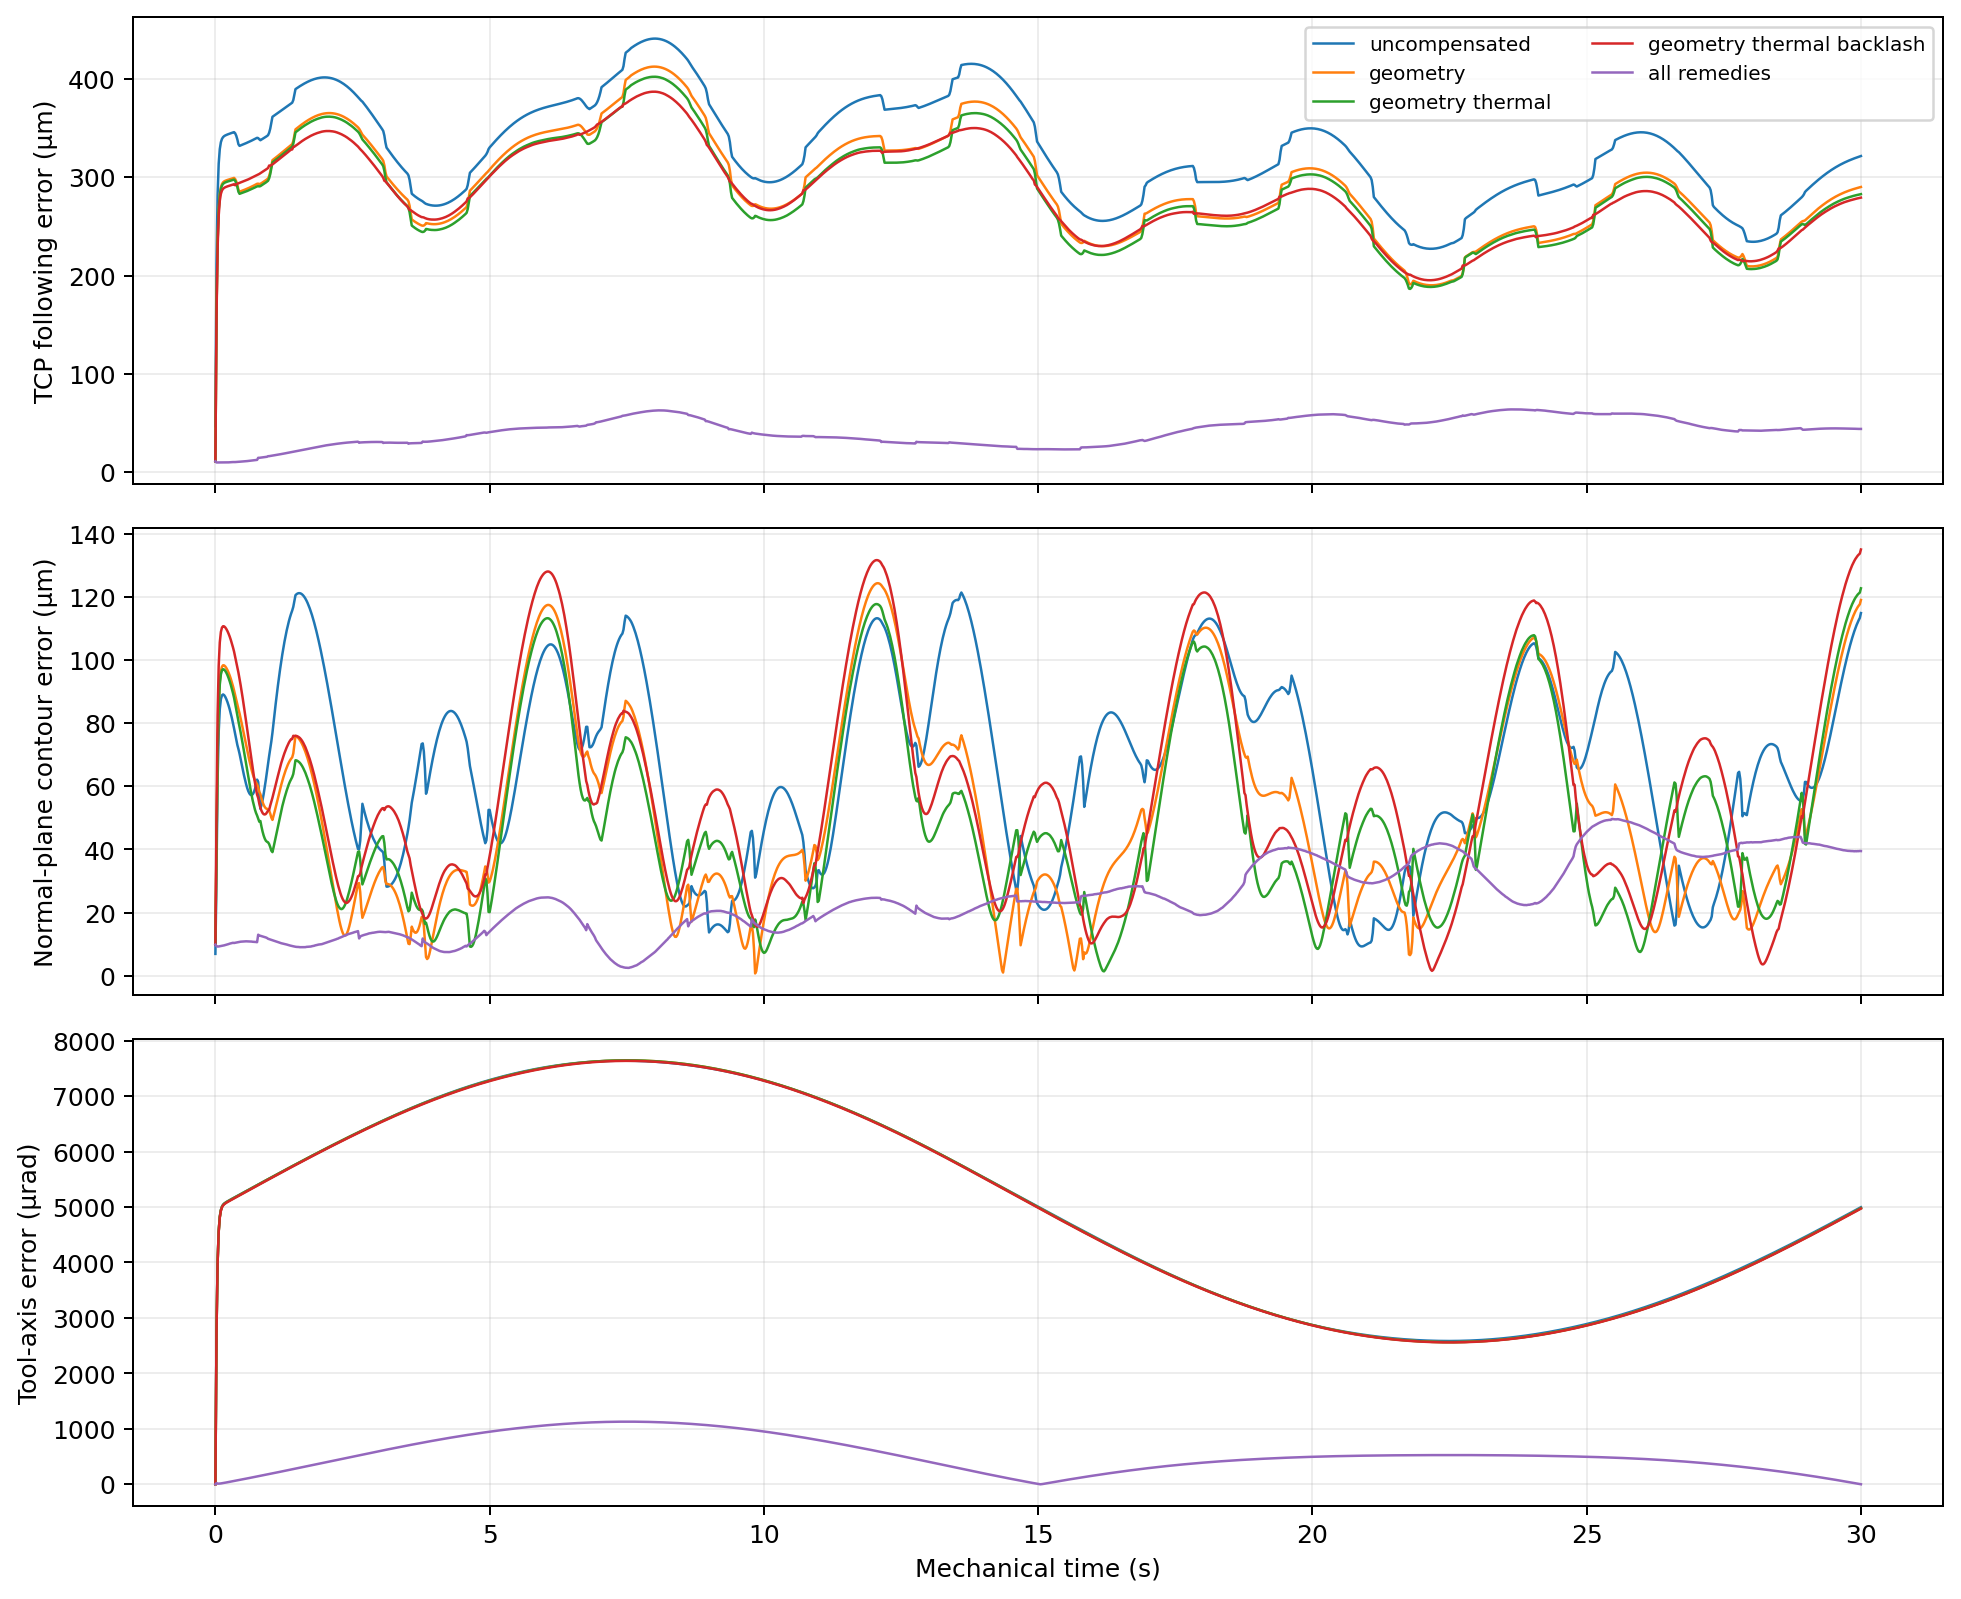
\includegraphics[width=.97\linewidth,height=73mm,keepaspectratio]{figures/research_integrated.png}\par\small\refstepcounter{figure}\textbf{Figure \thefigure.} Cumulative remedies and three trajectory error measures.\end{center}

\begin{center}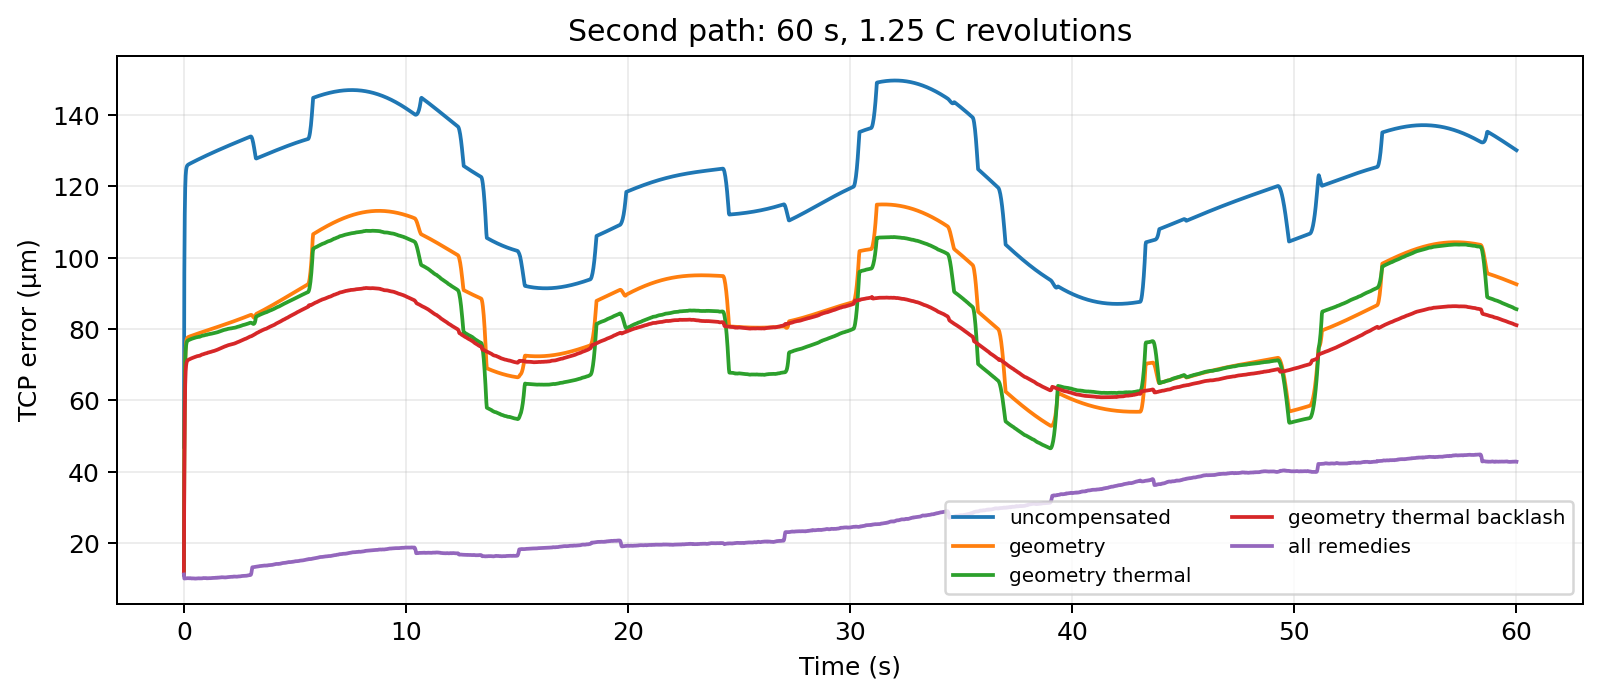
\includegraphics[width=.97\linewidth,height=73mm,keepaspectratio]{figures/research_second_path.png}\par\small\refstepcounter{figure}\textbf{Figure \thefigure.} Held-out slower-path result with the earlier drive model.\end{center}

\clearpage

\subsection{Which measurement observes which error?}

The drive command, motor encoder and output scale describe different points in the mechanical chain. The command-to-motor residual mainly exposes drive tracking, while output-minus-motor reveals play. Temperature channels are used to estimate drift. A separate XYZ probe evaluates the final motion; using it to tune the same trace would invalidate its role as an independent assessment.

\par{\small\textit{Implementation}\quad \file{dynamic_sim.py}\enspace /\enspace \file{research_experiments.py}}\par

\begin{center}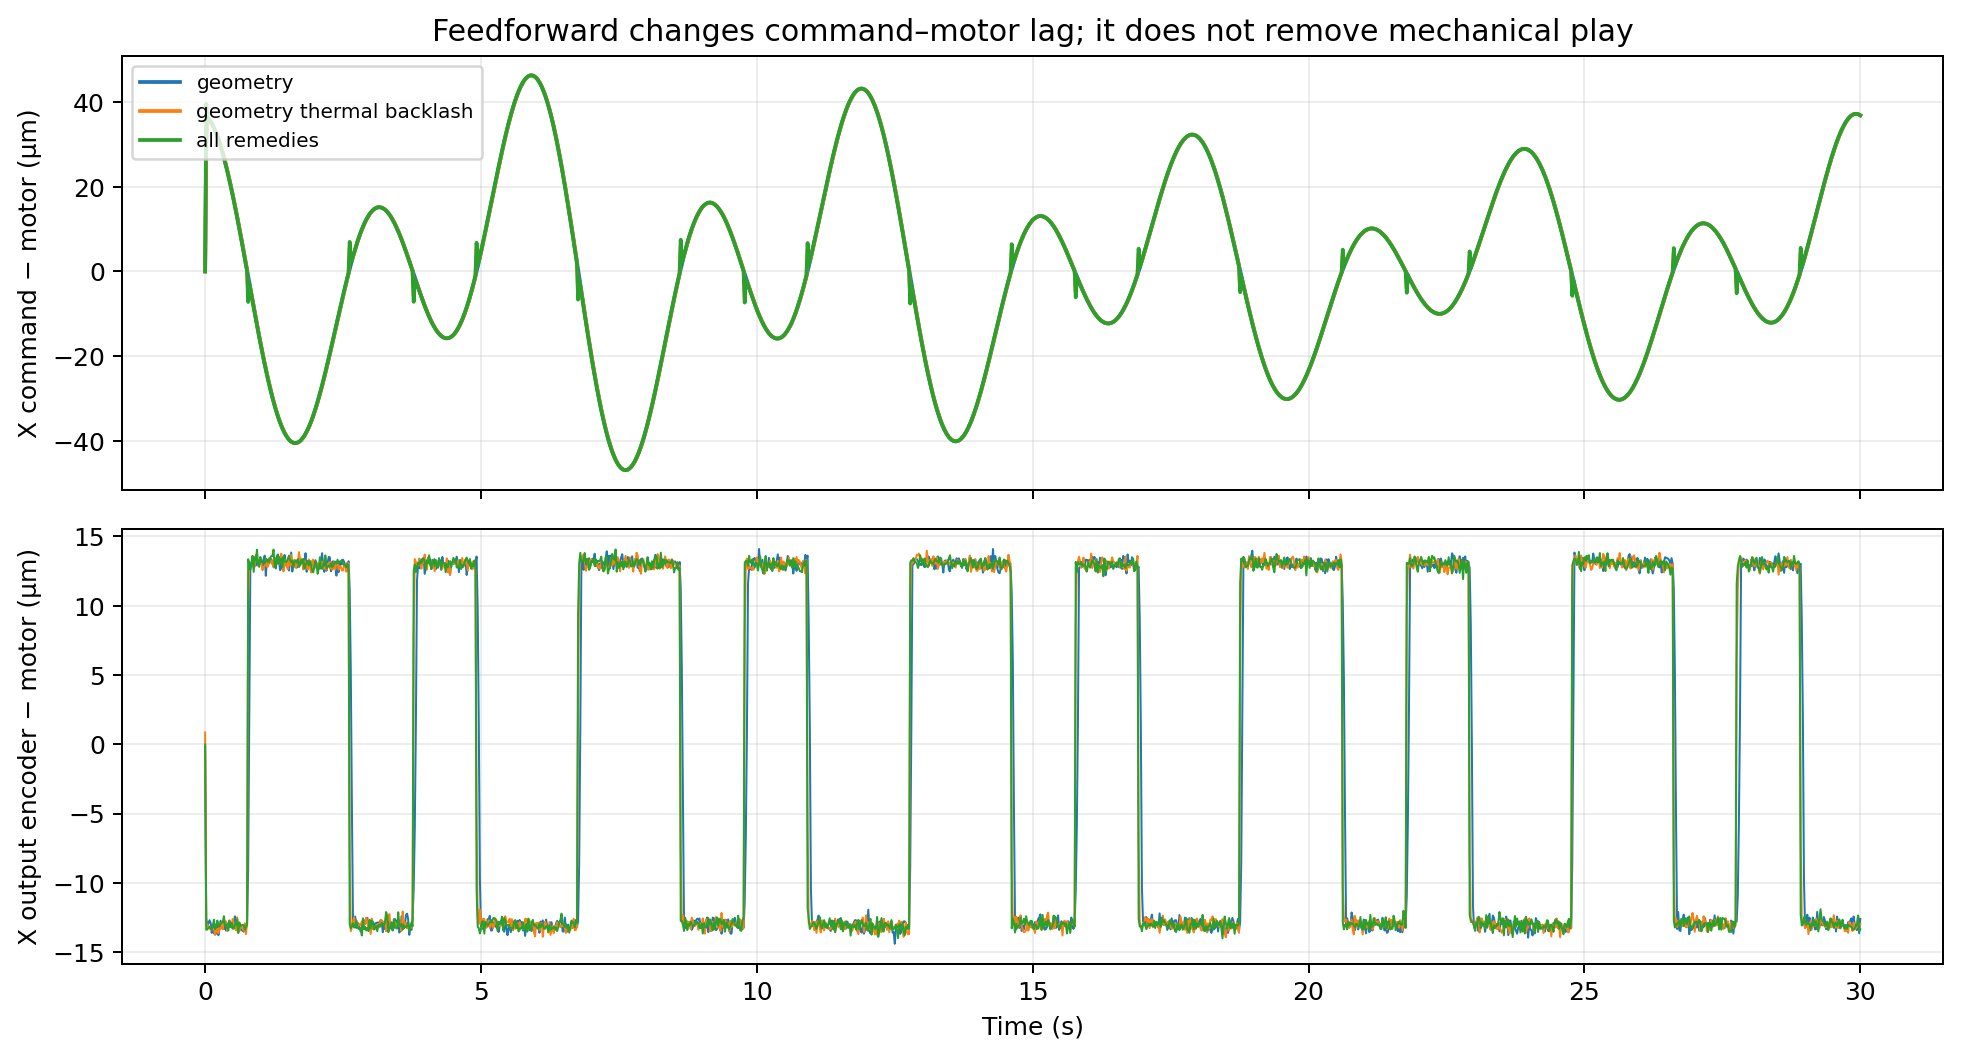
\includegraphics[width=.97\linewidth,height=73mm,keepaspectratio]{figures/research_encoder_sensors.png}\par\small\refstepcounter{figure}\textbf{Figure \thefigure.} Differences between motor and output measurements near reversals.\end{center}

\begin{center}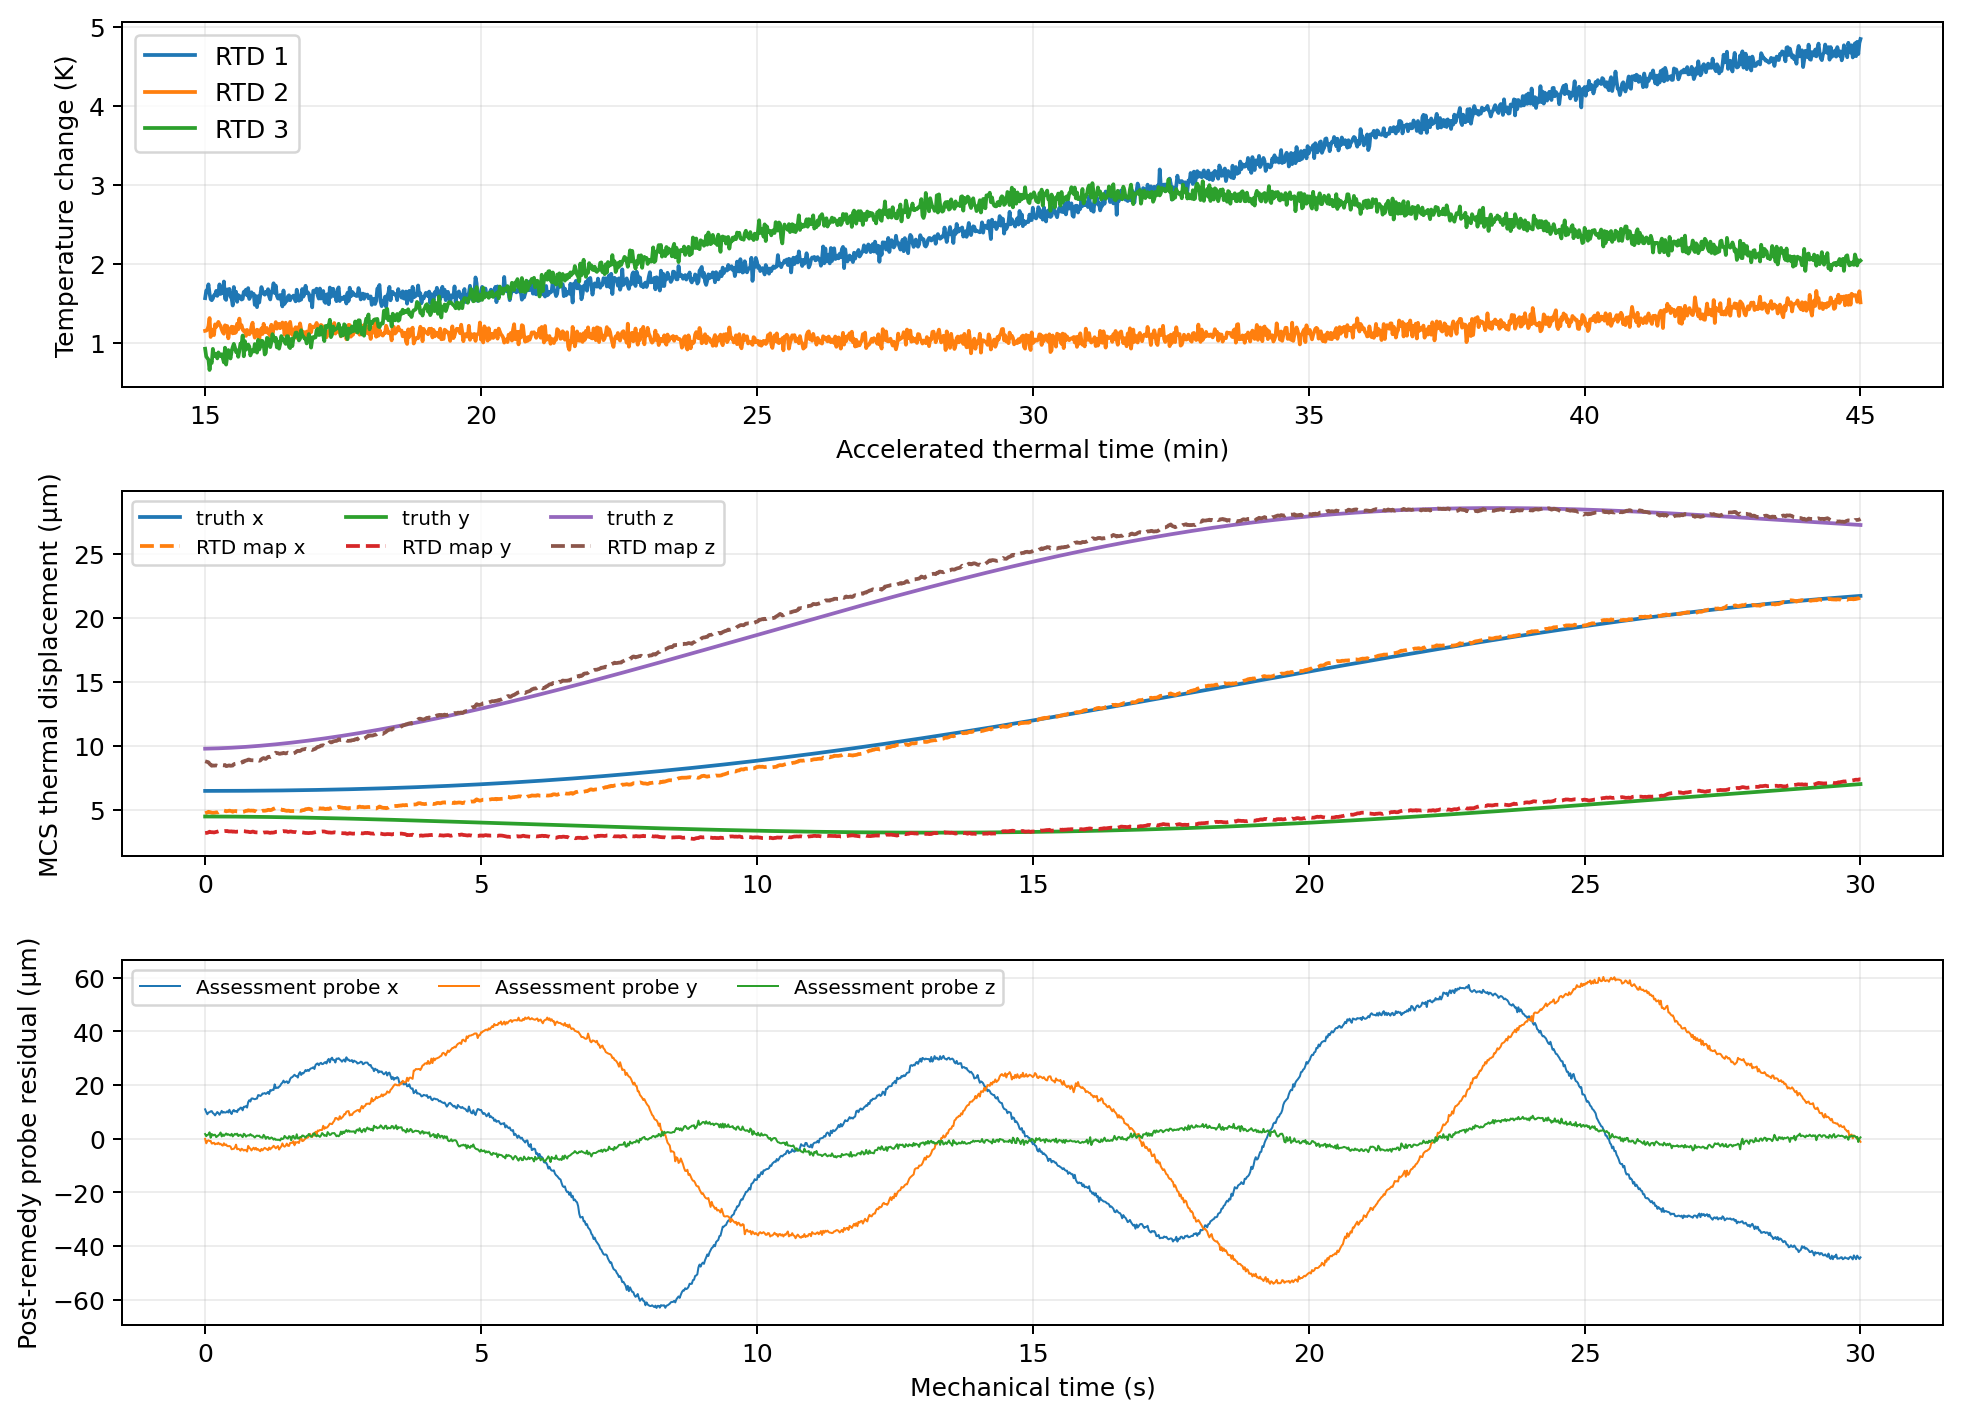
\includegraphics[width=.97\linewidth,height=73mm,keepaspectratio]{figures/research_thermal_sensors.png}\par\small\refstepcounter{figure}\textbf{Figure \thefigure.} Temperatures, inferred drift and independent position readout.\end{center}

\clearpage

\subsection{Two thermal clocks on a 30-second cut}

The physical-clock run advances temperature by 30 seconds during 30 seconds of motion. The accelerated run advances a 30-minute thermal scenario over those same mechanical commands. Physical-clock TCP RMS falls from 458.45 to 39.38 micrometres with all remedies. Under accelerated heating, the untreated RMS is 464.07. Separating the clocks exposes the interaction of thermal lag and feedforward.

\par{\small\textit{Implementation}\quad \file{publication_studies.py}\enspace /\enspace \file{dynamic_sim.py}}\par

\begin{center}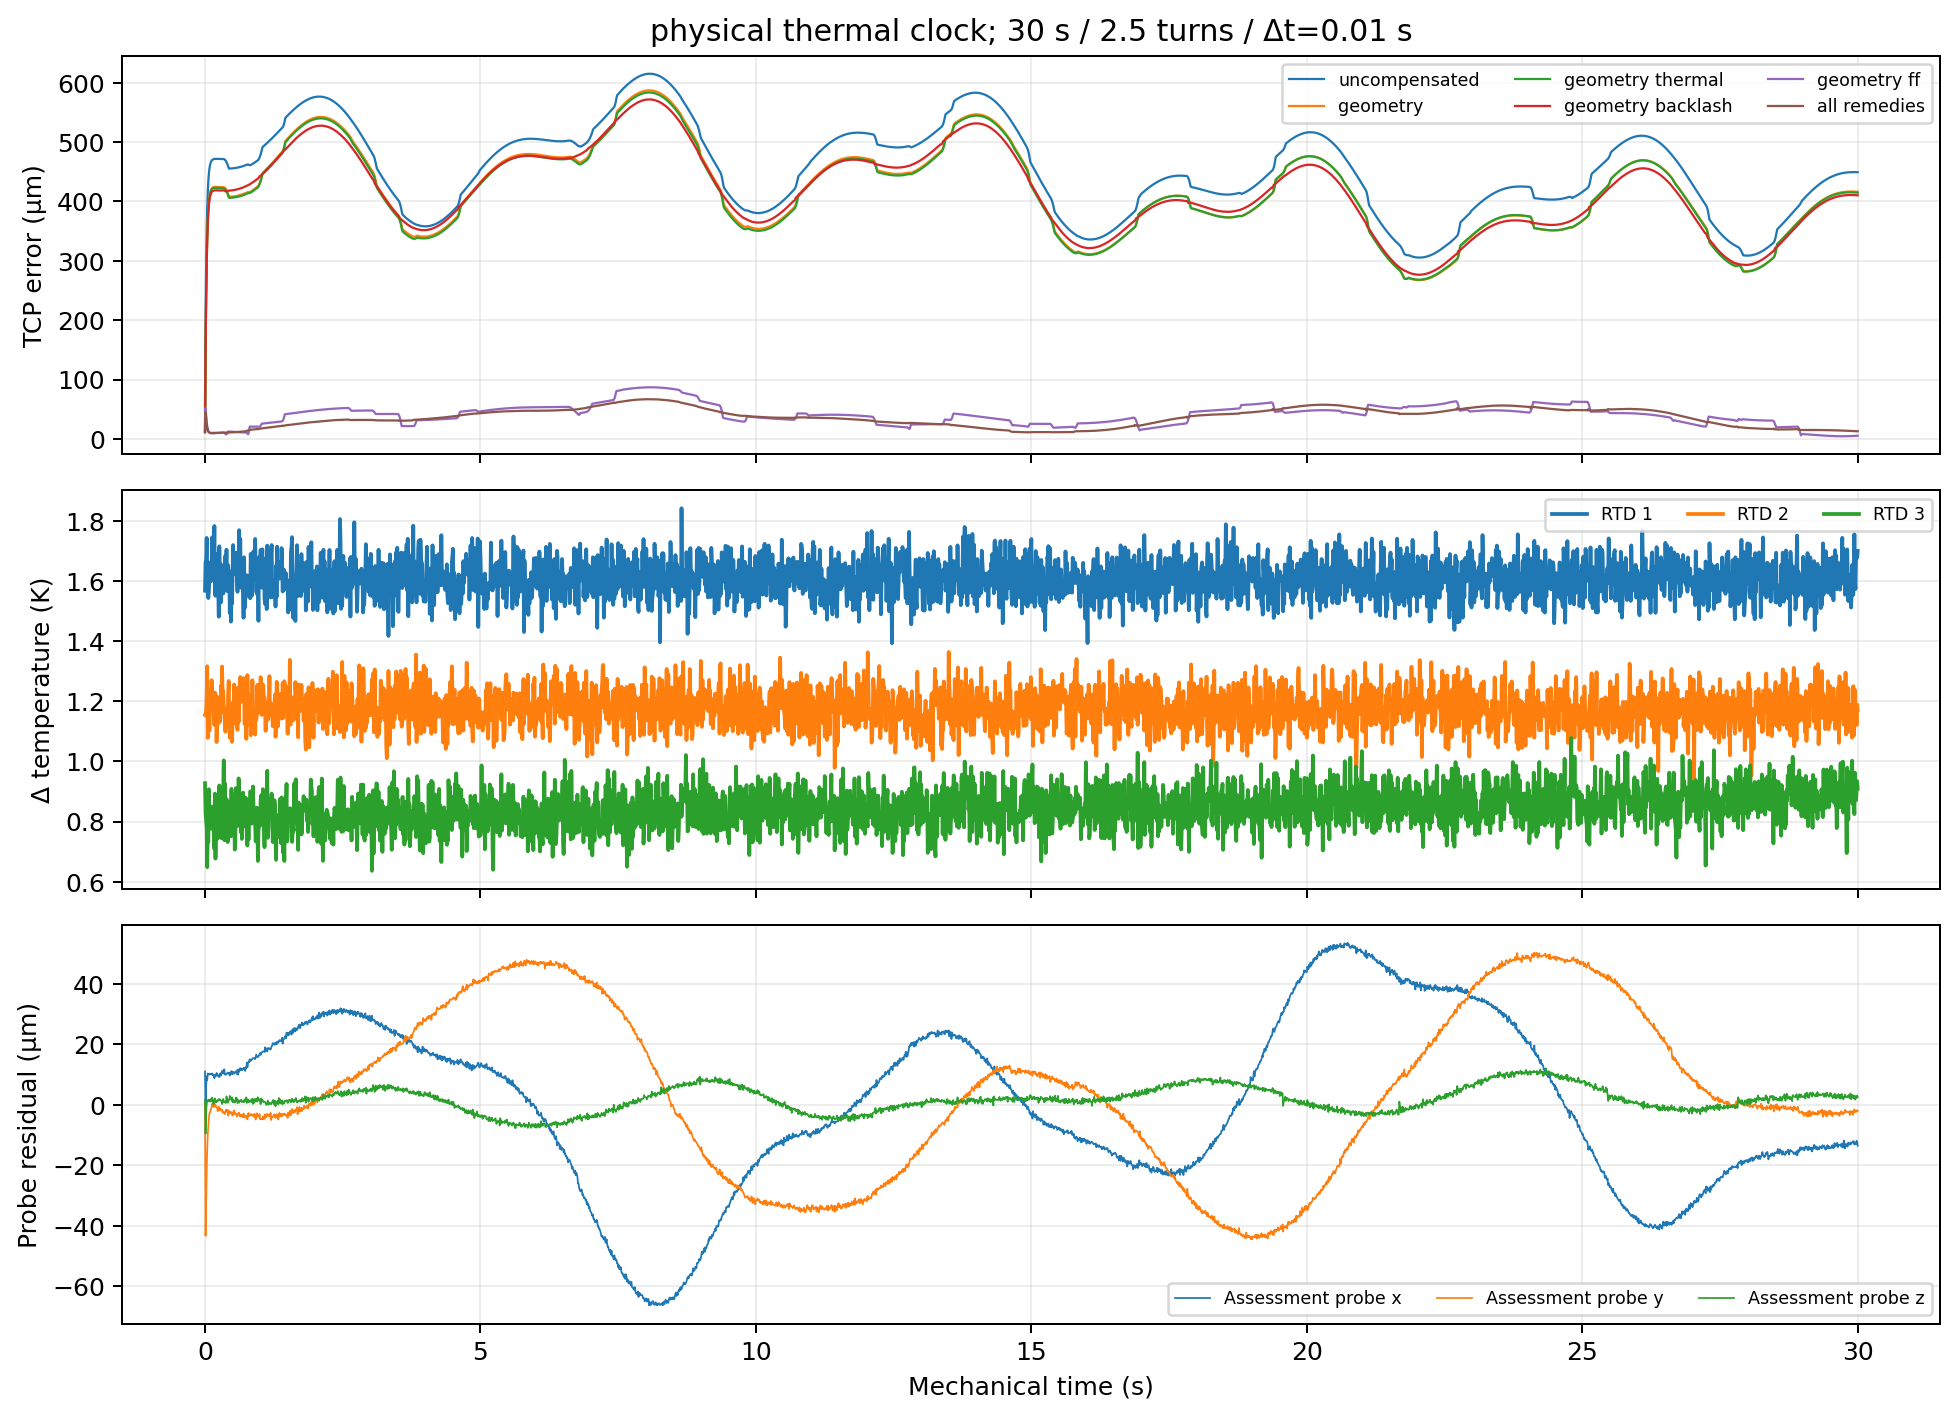
\includegraphics[width=.97\linewidth,height=73mm,keepaspectratio]{figures/publication_dynamic_physical_30.png}\par\small\refstepcounter{figure}\textbf{Figure \thefigure.} Executed path and sensor traces with physical thermal time.\end{center}

\begin{center}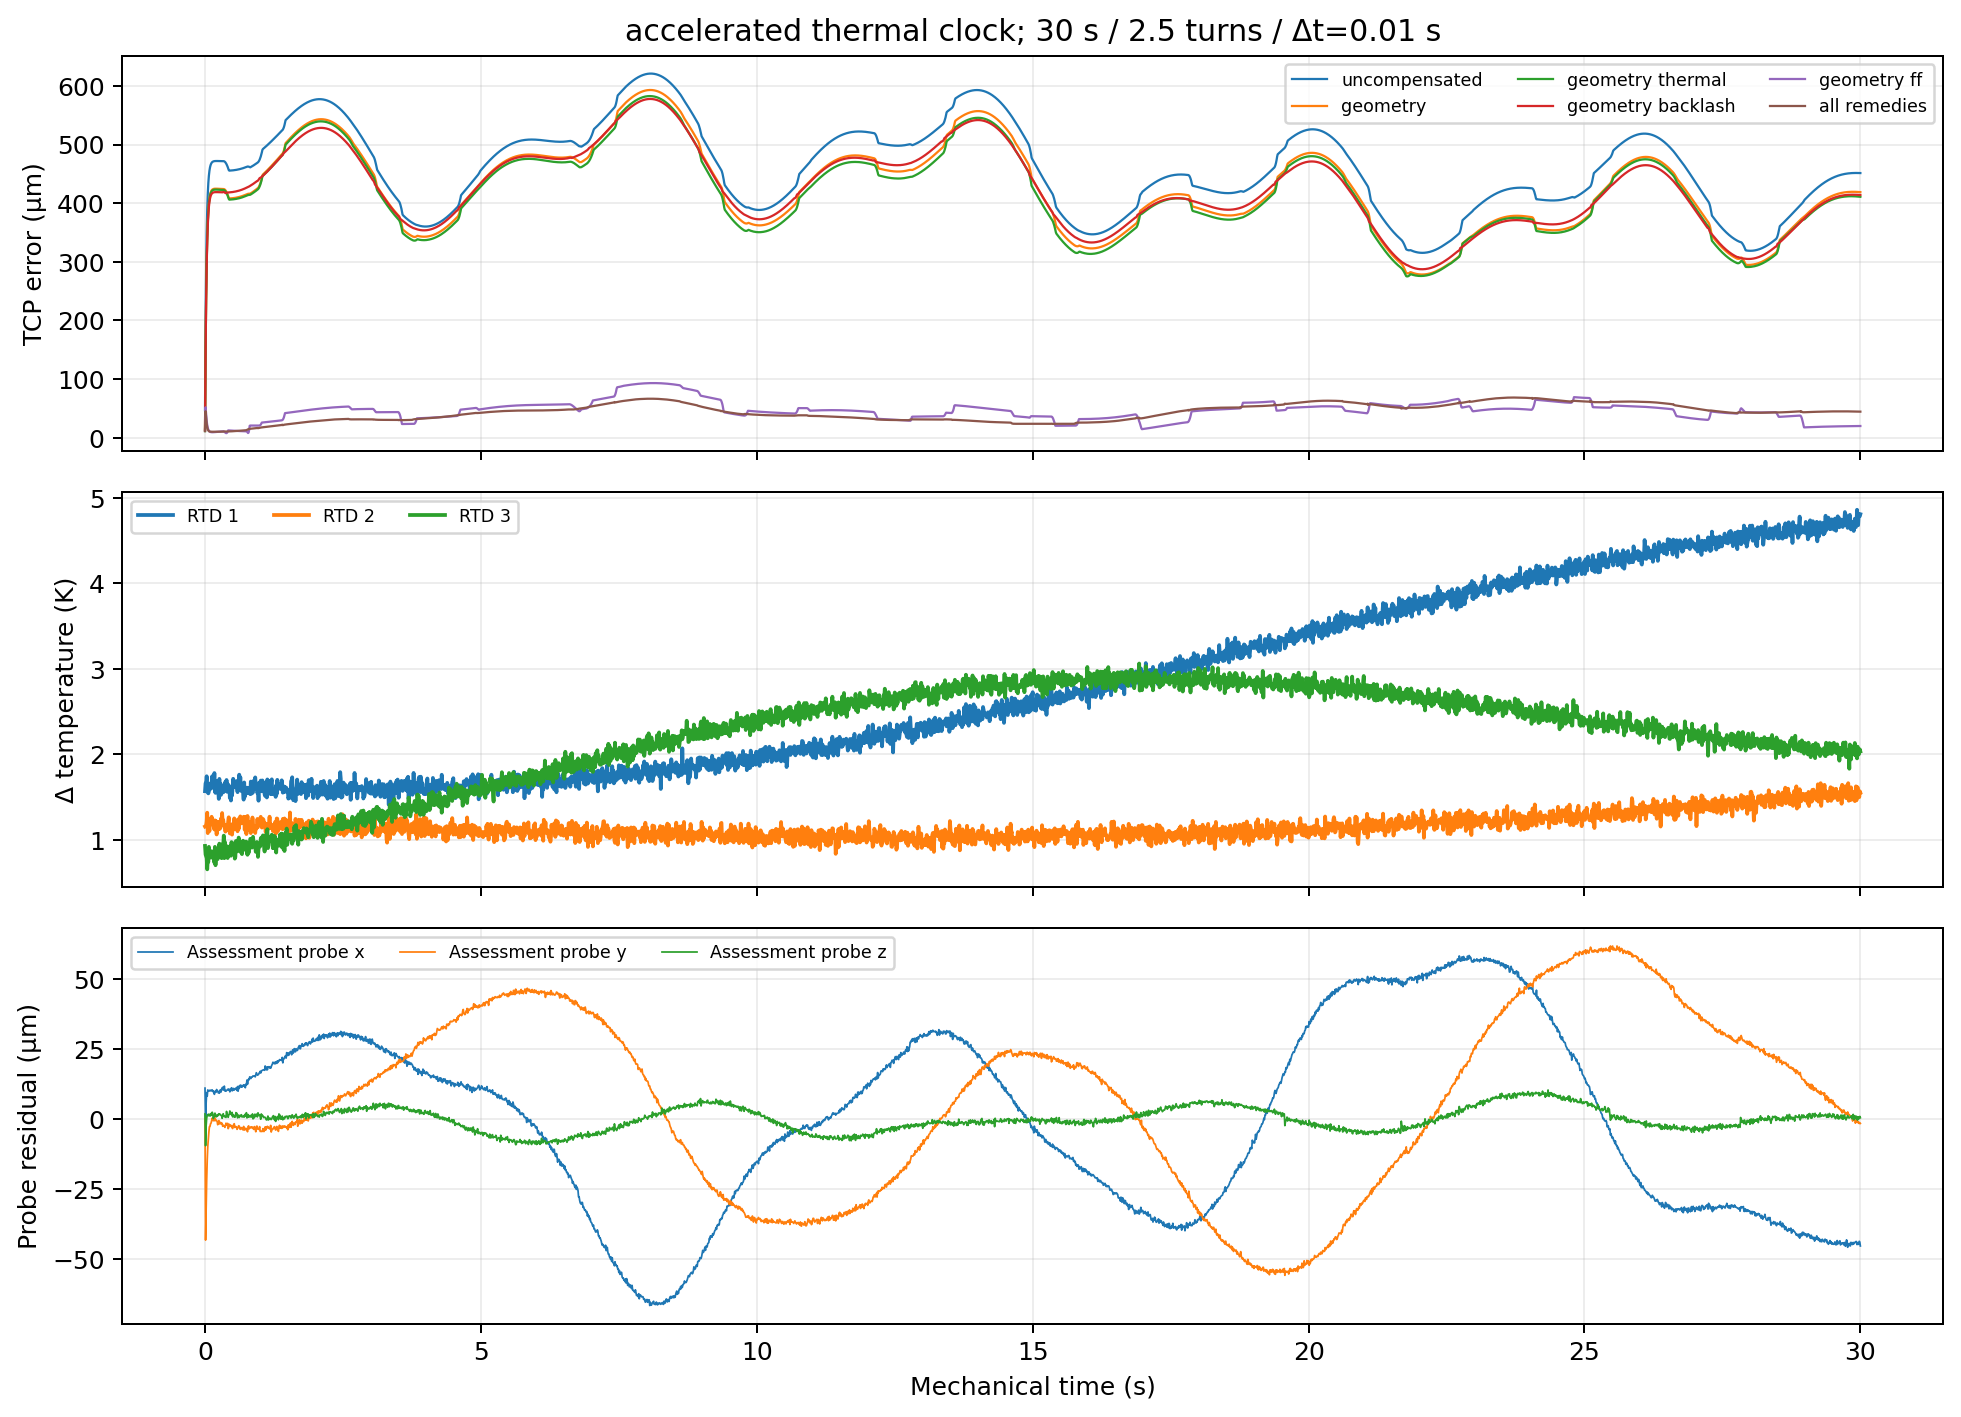
\includegraphics[width=.97\linewidth,height=73mm,keepaspectratio]{figures/publication_dynamic_accelerated_30.png}\par\small\refstepcounter{figure}\textbf{Figure \thefigure.} Same motion under accelerated thermal evolution.\end{center}

\clearpage

\subsection{Checking speed and numerical resolution}

The held-out 60 s, 1.25-turn path changes the excitation while preserving the declared calibration protocol. A separate grid study fixes fitted time constants and uses nested RTD noise. As the time step is halved from 0.005 to 0.0025 s, physical-clock full-remedy TCP RMS changes from 39.431 to 39.433 micrometres in that grid test. This checks sensitivity to sampling near the stated resolution.

\par{\small\textit{Implementation}\quad \file{publication_studies.py}\enspace /\enspace \file{dynamic_sim.py}}\par

\begin{center}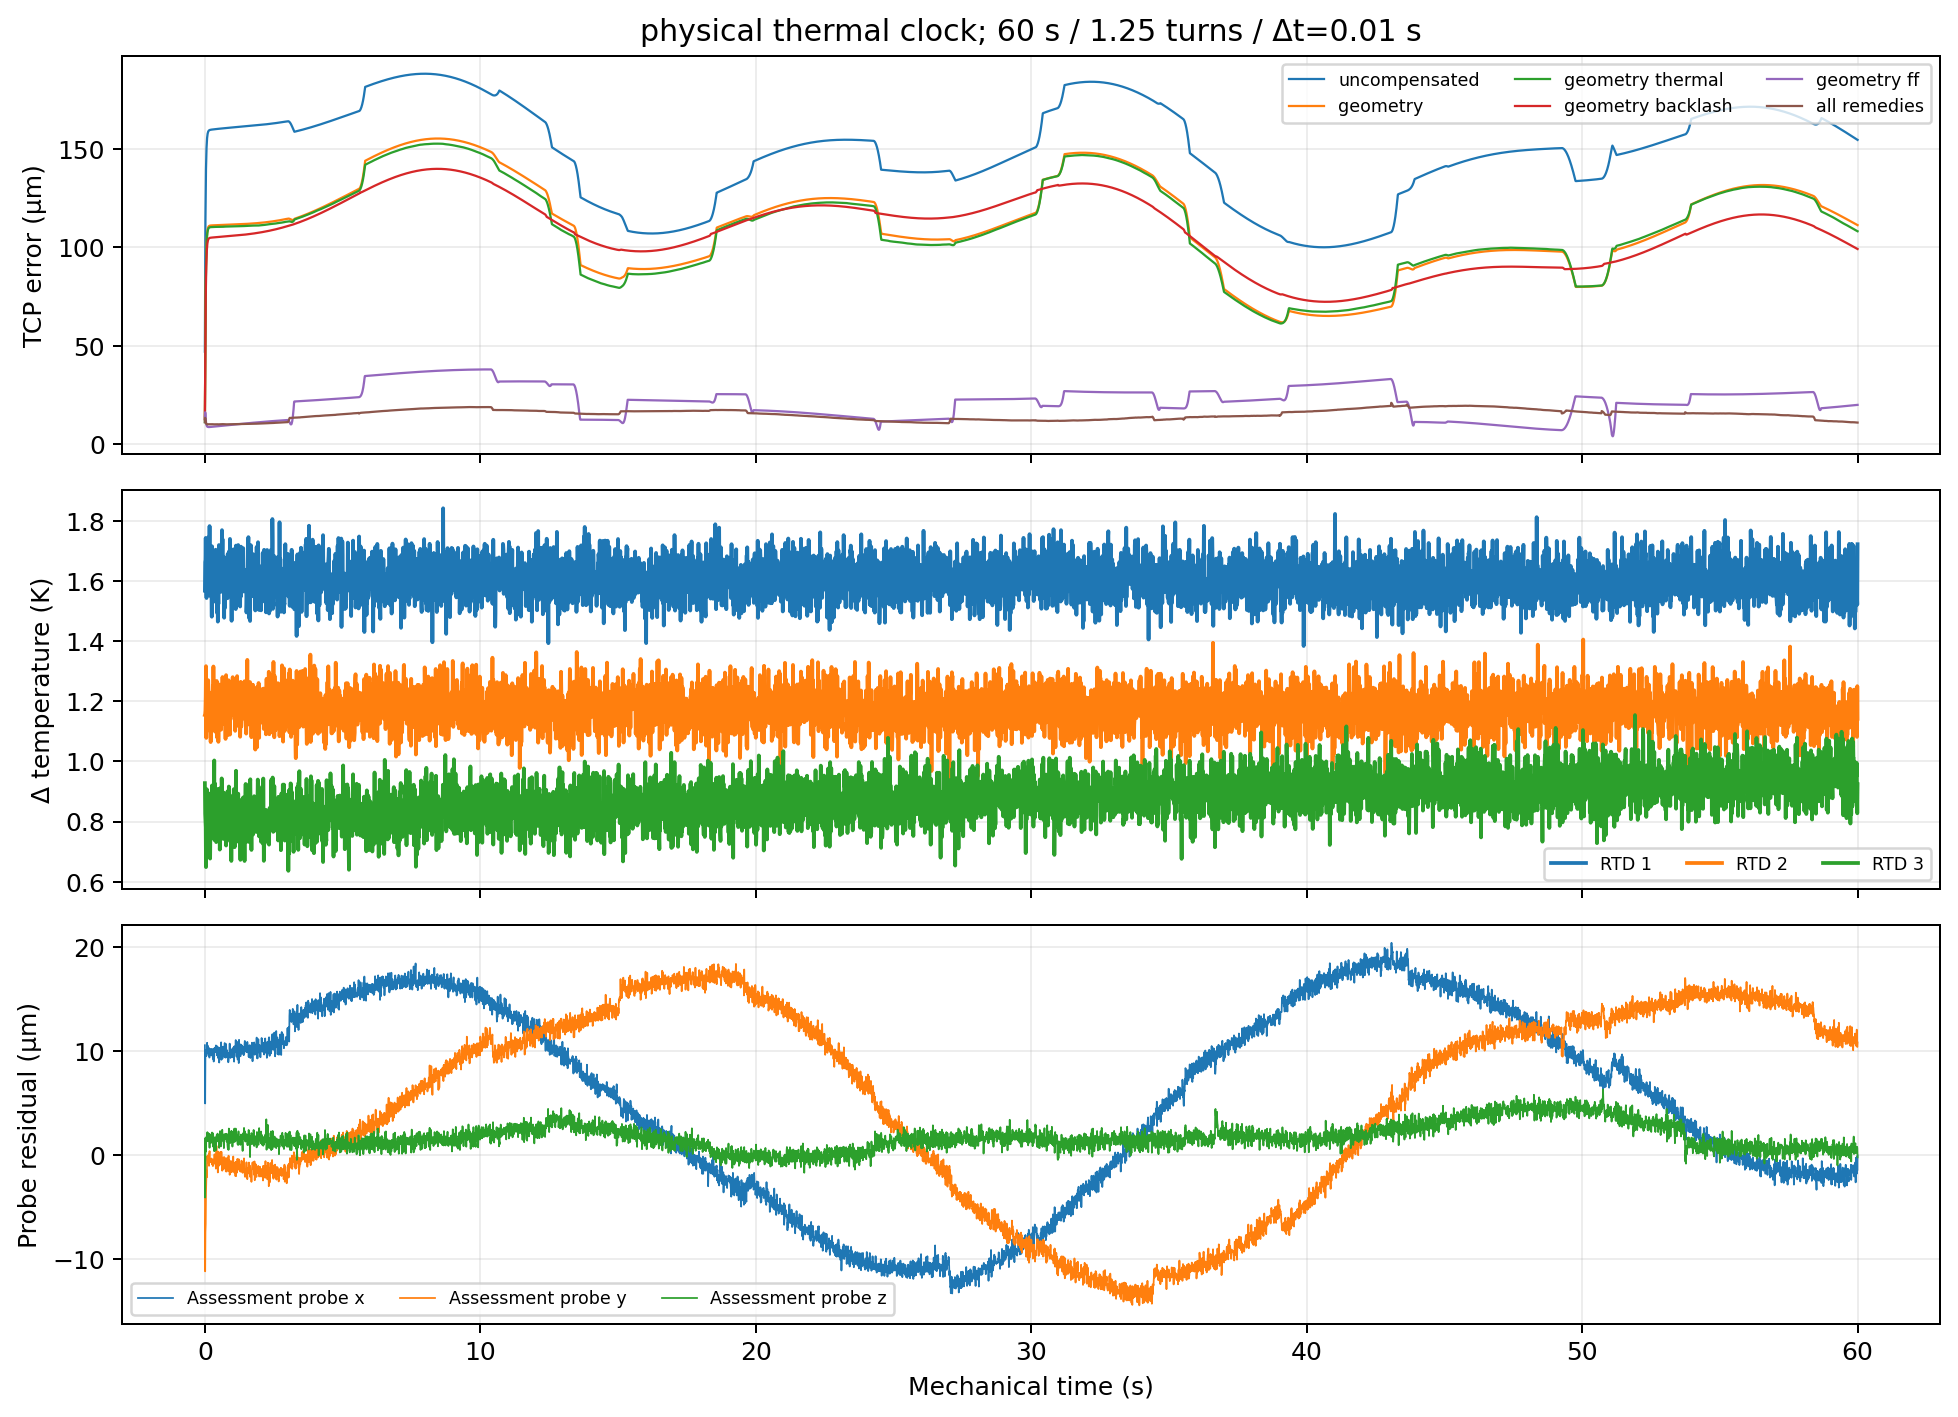
\includegraphics[width=.97\linewidth,height=47mm,keepaspectratio]{figures/publication_dynamic_physical_60.png}\par\small\refstepcounter{figure}\textbf{Figure \thefigure.} Held-out slower path with physical thermal time.\end{center}

\begin{center}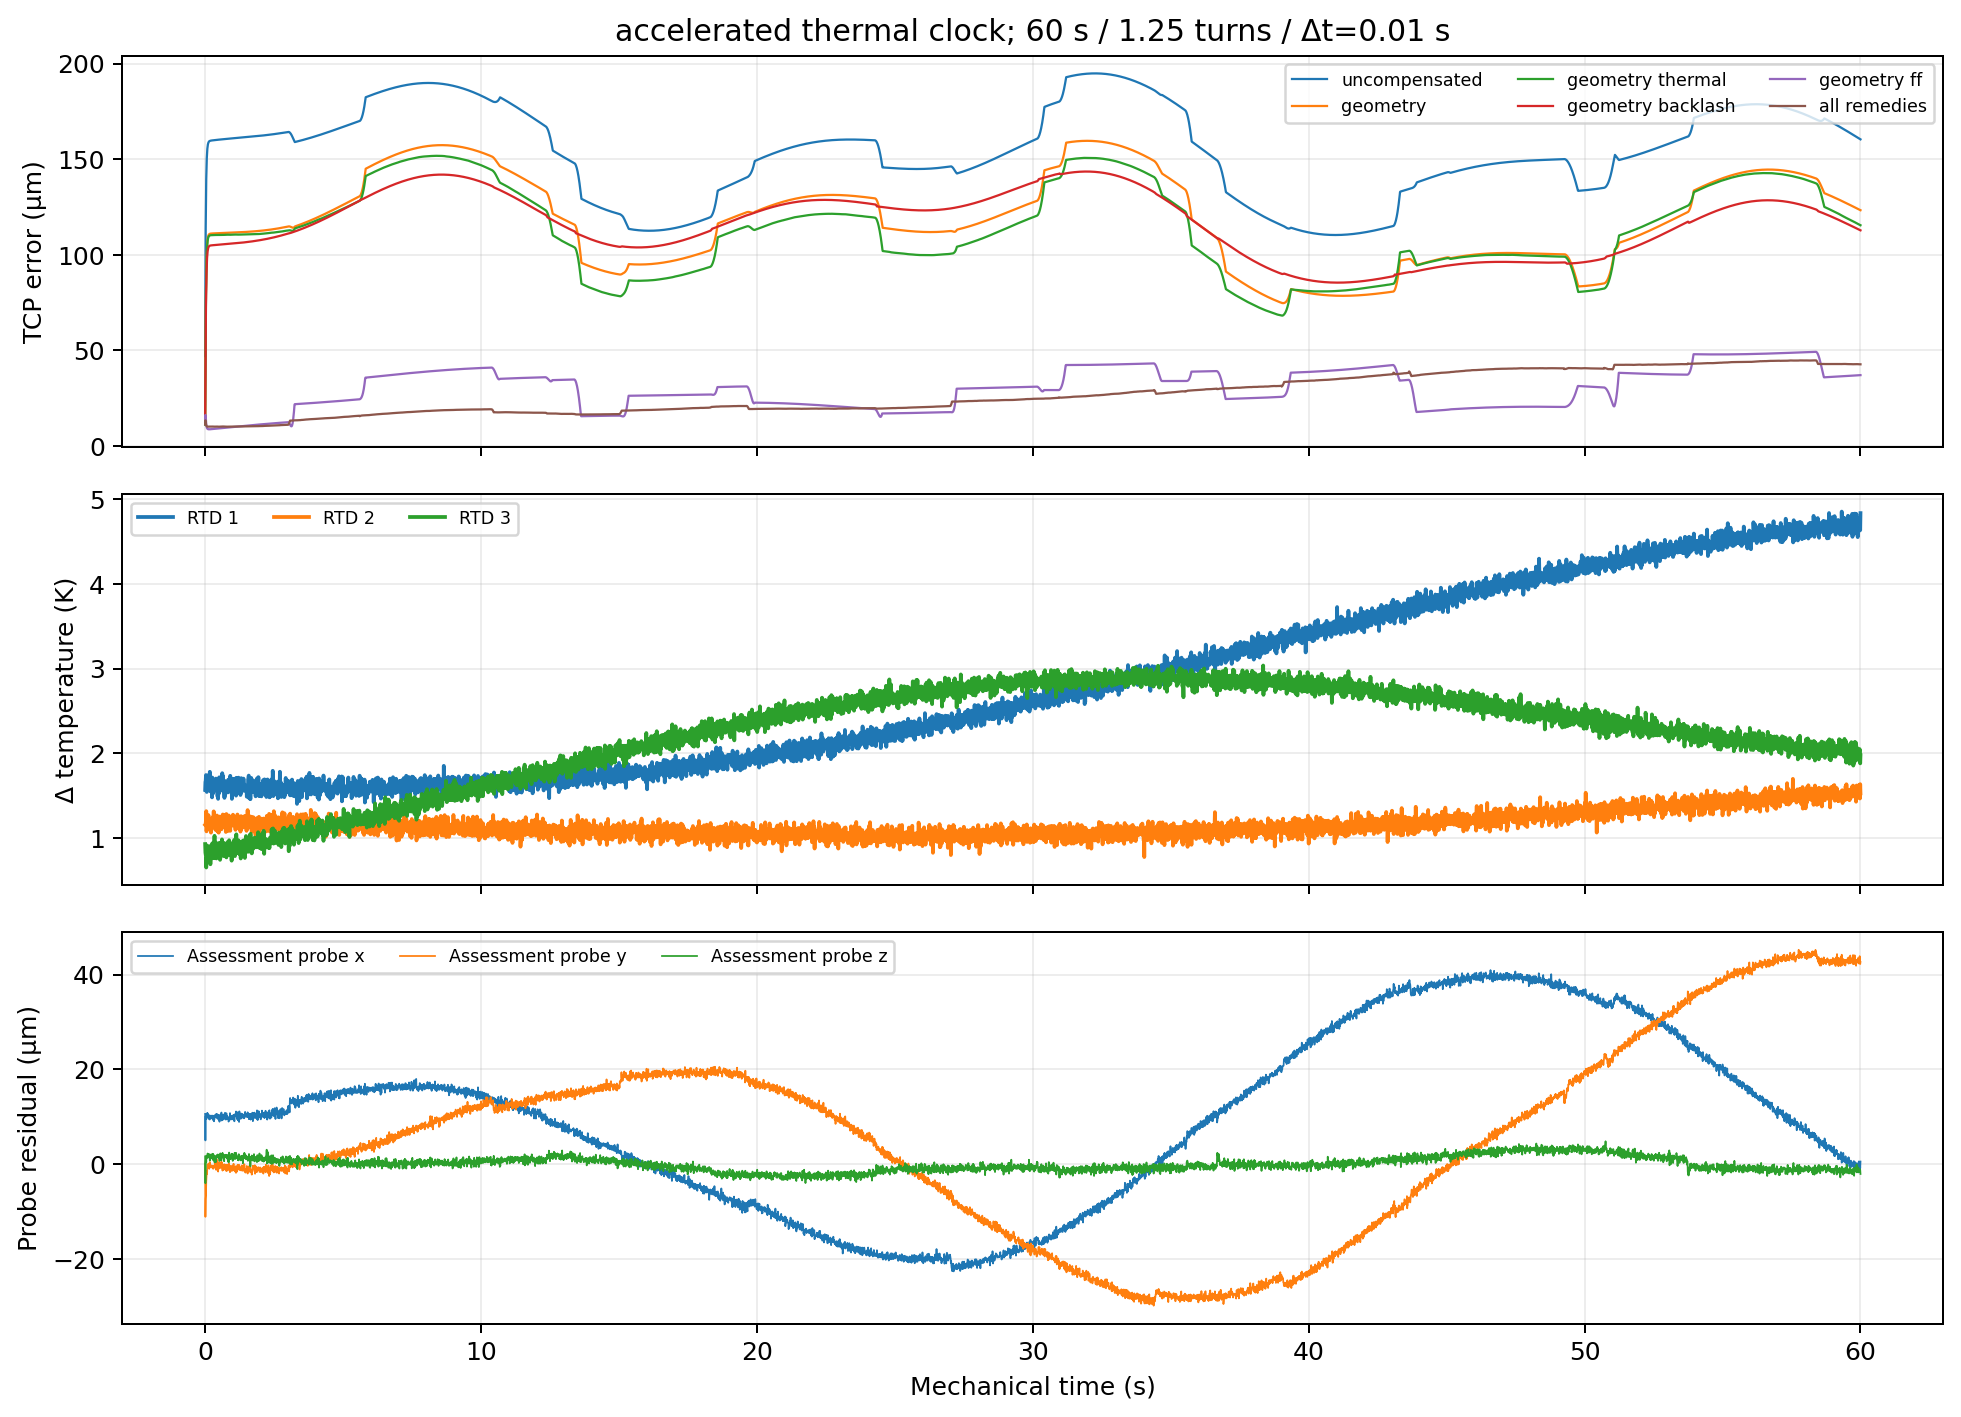
\includegraphics[width=.97\linewidth,height=47mm,keepaspectratio]{figures/publication_dynamic_accelerated_60.png}\par\small\refstepcounter{figure}\textbf{Figure \thefigure.} Slower path under accelerated thermal stress.\end{center}

\begin{center}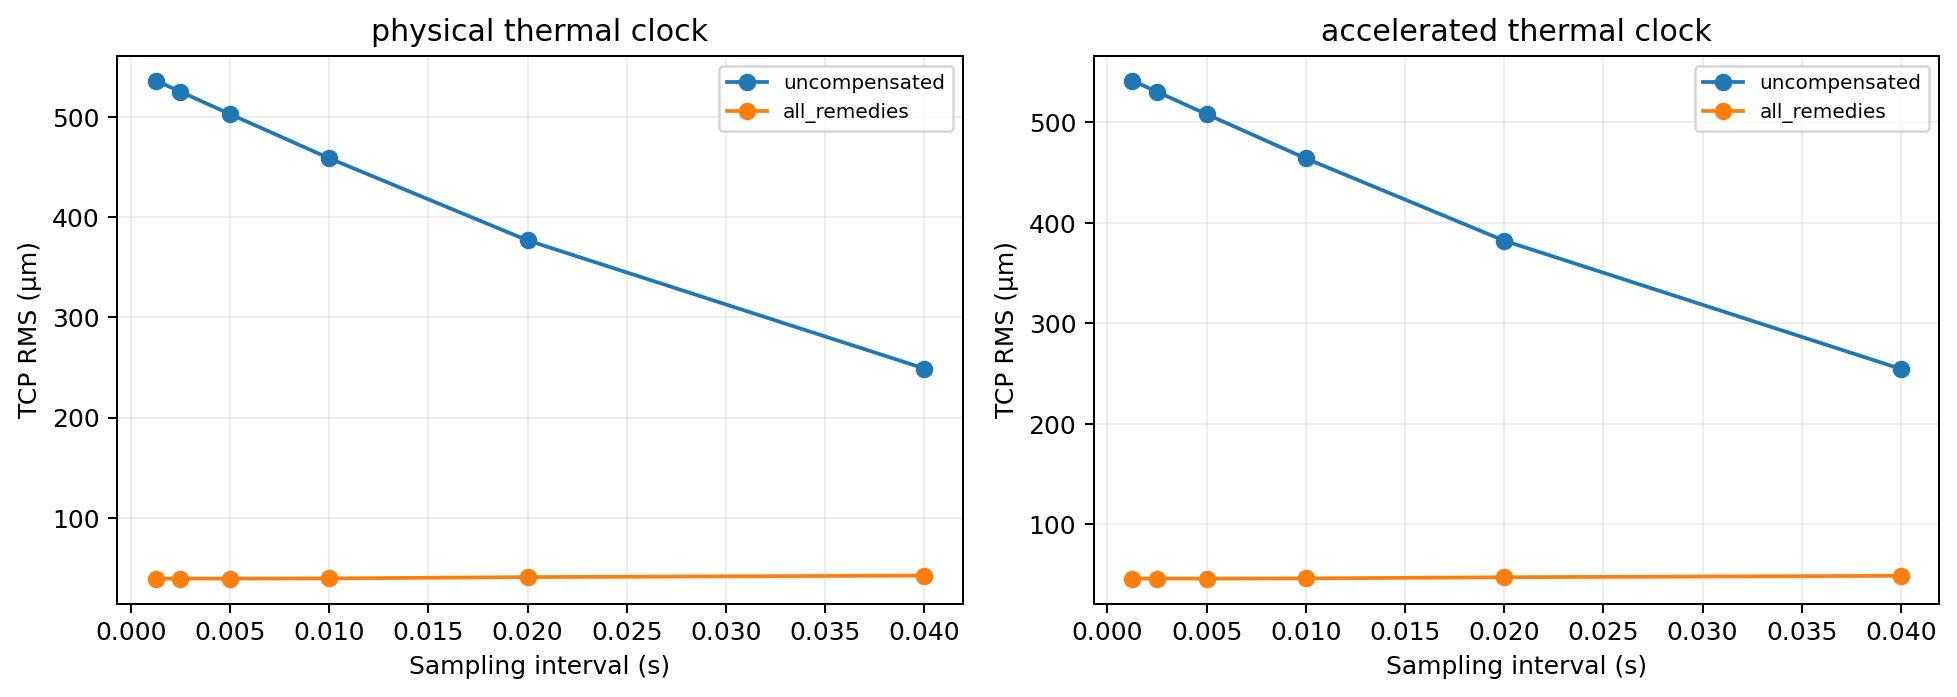
\includegraphics[width=.97\linewidth,height=47mm,keepaspectratio]{figures/publication_sampling_convergence.png}\par\small\refstepcounter{figure}\textbf{Figure \thefigure.} Discretization sensitivity of TCP and contour residuals.\end{center}

\clearpage

\section{Predictive uncertainty and inspection evidence}

\subsection{What a covariance check validates}

The first control draws noise from the same linear model used to calculate uncertainty. Agreement establishes that the propagation works under its assumptions. Repeating the experiment with independent nonlinear truth reveals a separate source of error: a bias can move the residual distribution away from zero while its spread remains small. Refining the covariance alone then leaves many observations outside the predicted region.

\par{\small\textit{Implementation}\quad \file{publication_studies.py}\enspace /\enspace \file{journal_models.py}}\par

\begin{center}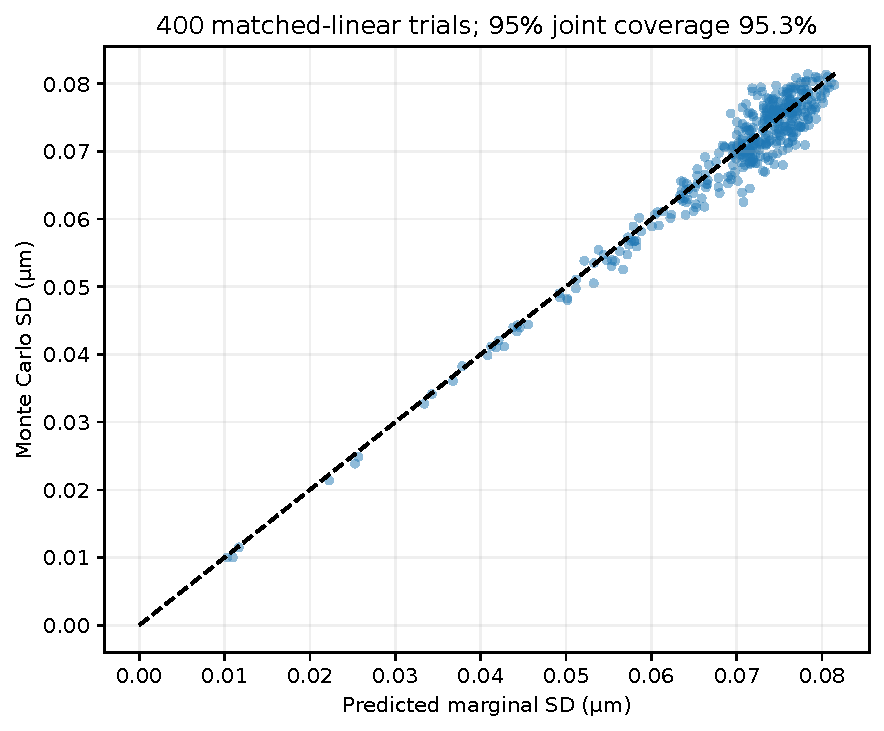
\includegraphics[width=.97\linewidth,height=73mm,keepaspectratio]{figures/publication_uncertainty_control.pdf}\par\small\refstepcounter{figure}\textbf{Figure \thefigure.} Conditional covariance compared with 400 matched-model Monte Carlo draws.\end{center}

\begin{center}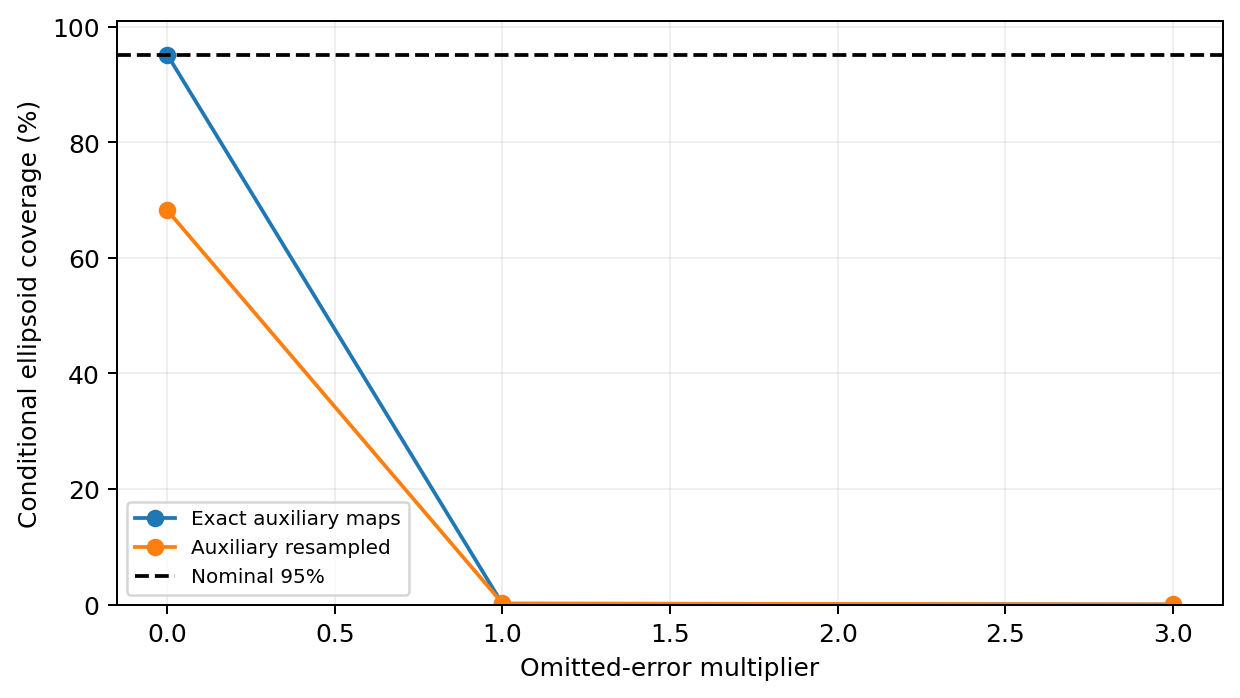
\includegraphics[width=.97\linewidth,height=73mm,keepaspectratio]{figures/publication_mismatch_coverage.png}\par\small\refstepcounter{figure}\textbf{Figure \thefigure.} Loss of coverage under omitted terms and auxiliary uncertainty.\end{center}

\clearpage

\subsection{Noise-free tool position versus a future probe reading}

In the earlier 3,600-fit audit, rotary-only propagation covers 56.13\% of matched latent TCPs; retaining shared auxiliary uncertainty gives 95.56\%. Including probe variance gives 94.97\% for the observed response. The assessment trace shows one coordinate projection. Joint coverage requires the full three-dimensional residual to fall in the ellipsoid, so counting points inside an X band overstates what that projection can establish.

\par{\small\textit{Implementation}\quad \file{journal_studies.py}\enspace /\enspace \file{journal_dashboard.py}}\par

\begin{center}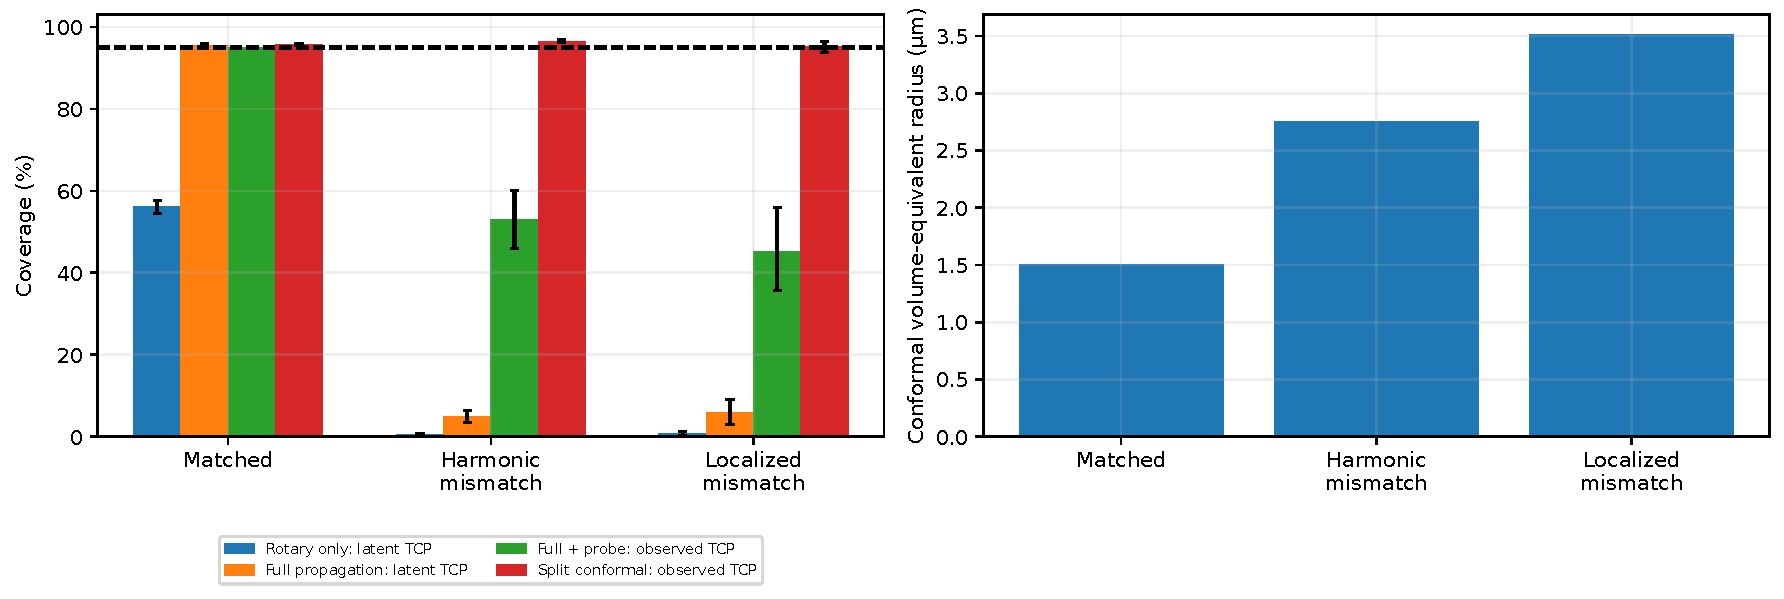
\includegraphics[width=.97\linewidth,height=73mm,keepaspectratio]{figures/journal_tcp_coverage.pdf}\par\small\refstepcounter{figure}\textbf{Figure \thefigure.} Latent and observed-target coverage in the earlier audit.\end{center}

\begin{center}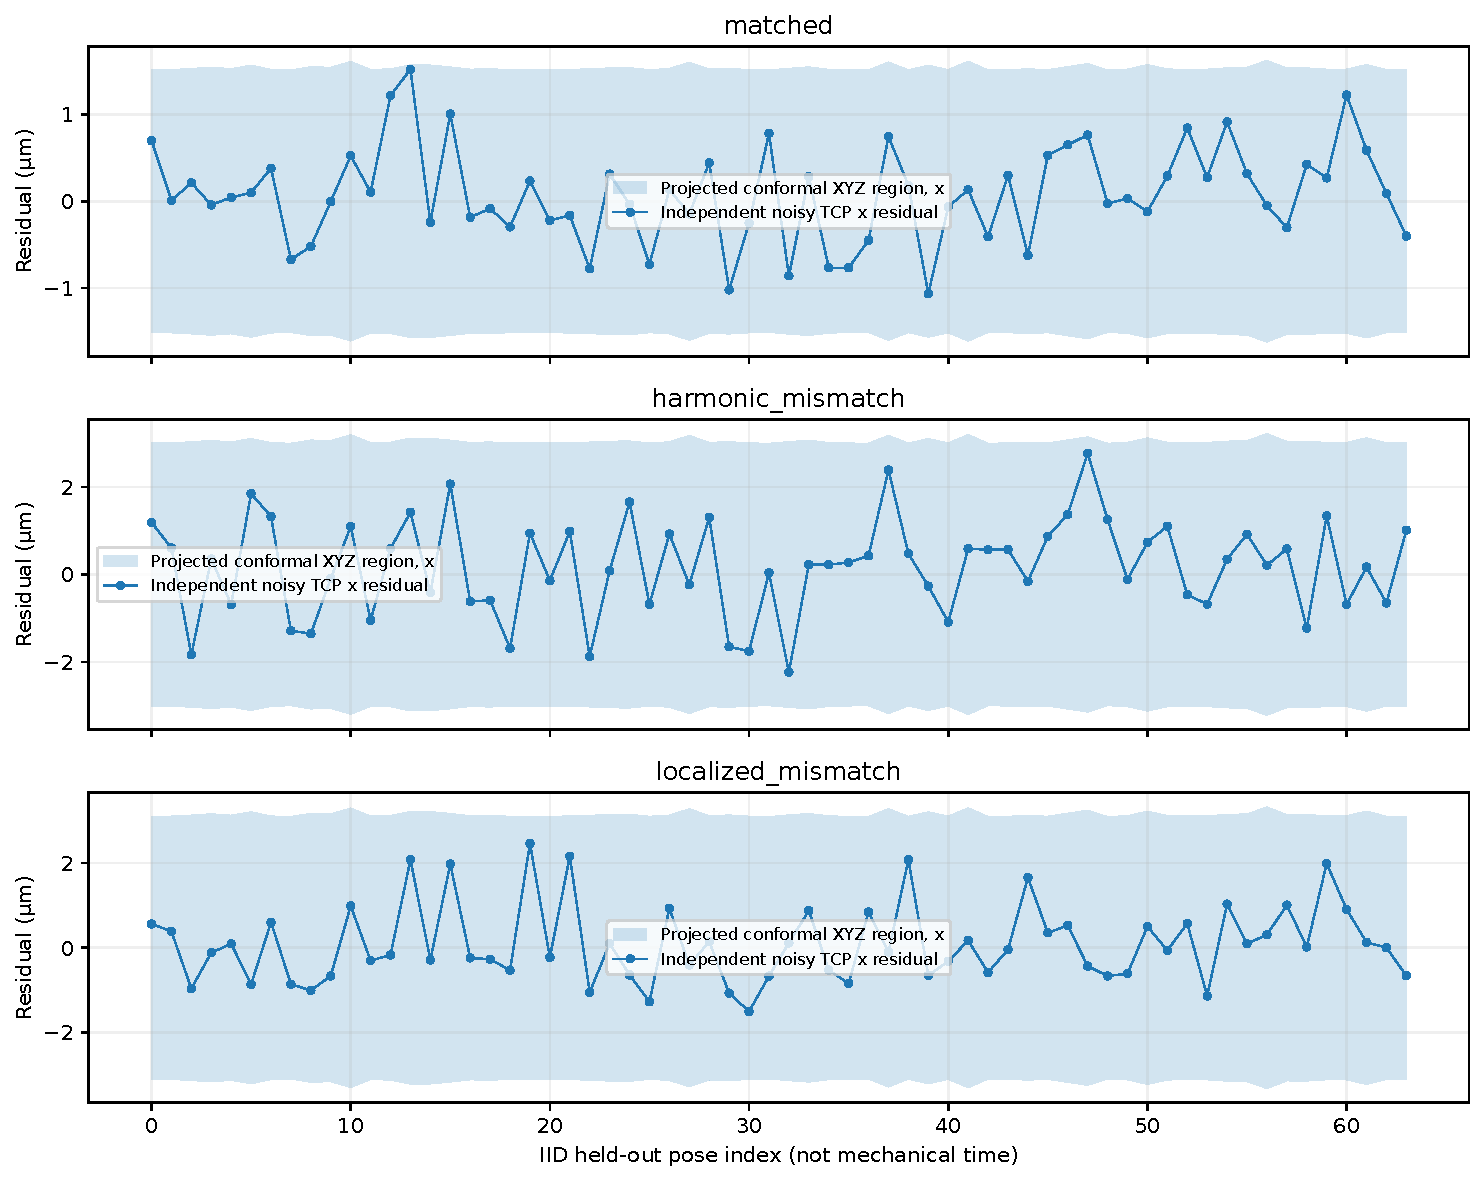
\includegraphics[width=.97\linewidth,height=73mm,keepaspectratio]{figures/journal_prediction_regions.pdf}\par\small\refstepcounter{figure}\textbf{Figure \thefigure.} X residuals and projected XYZ regions for independently drawn commands.\end{center}

\clearpage

\subsection{Comparing seven predictive regions}

The seven methods share fitted positions and assessment responses. Deleting only the fitted cross-covariance while preserving both marginal blocks raises matched independent-noise coverage to 98.05\% and mean radius from 1.449 to 1.651 micrometres. The nonlinear covariance differs from the joint first-order one by 5.82\% in relative Frobenius norm on average; the two half-samples differ by 11.29\%. The probe variance contributes to the close agreement of the Gaussian coverage values.

\par{\small\textit{Implementation}\quad \file{audit_models.py}\enspace /\enspace \file{audit_studies.py}}\par

\begin{center}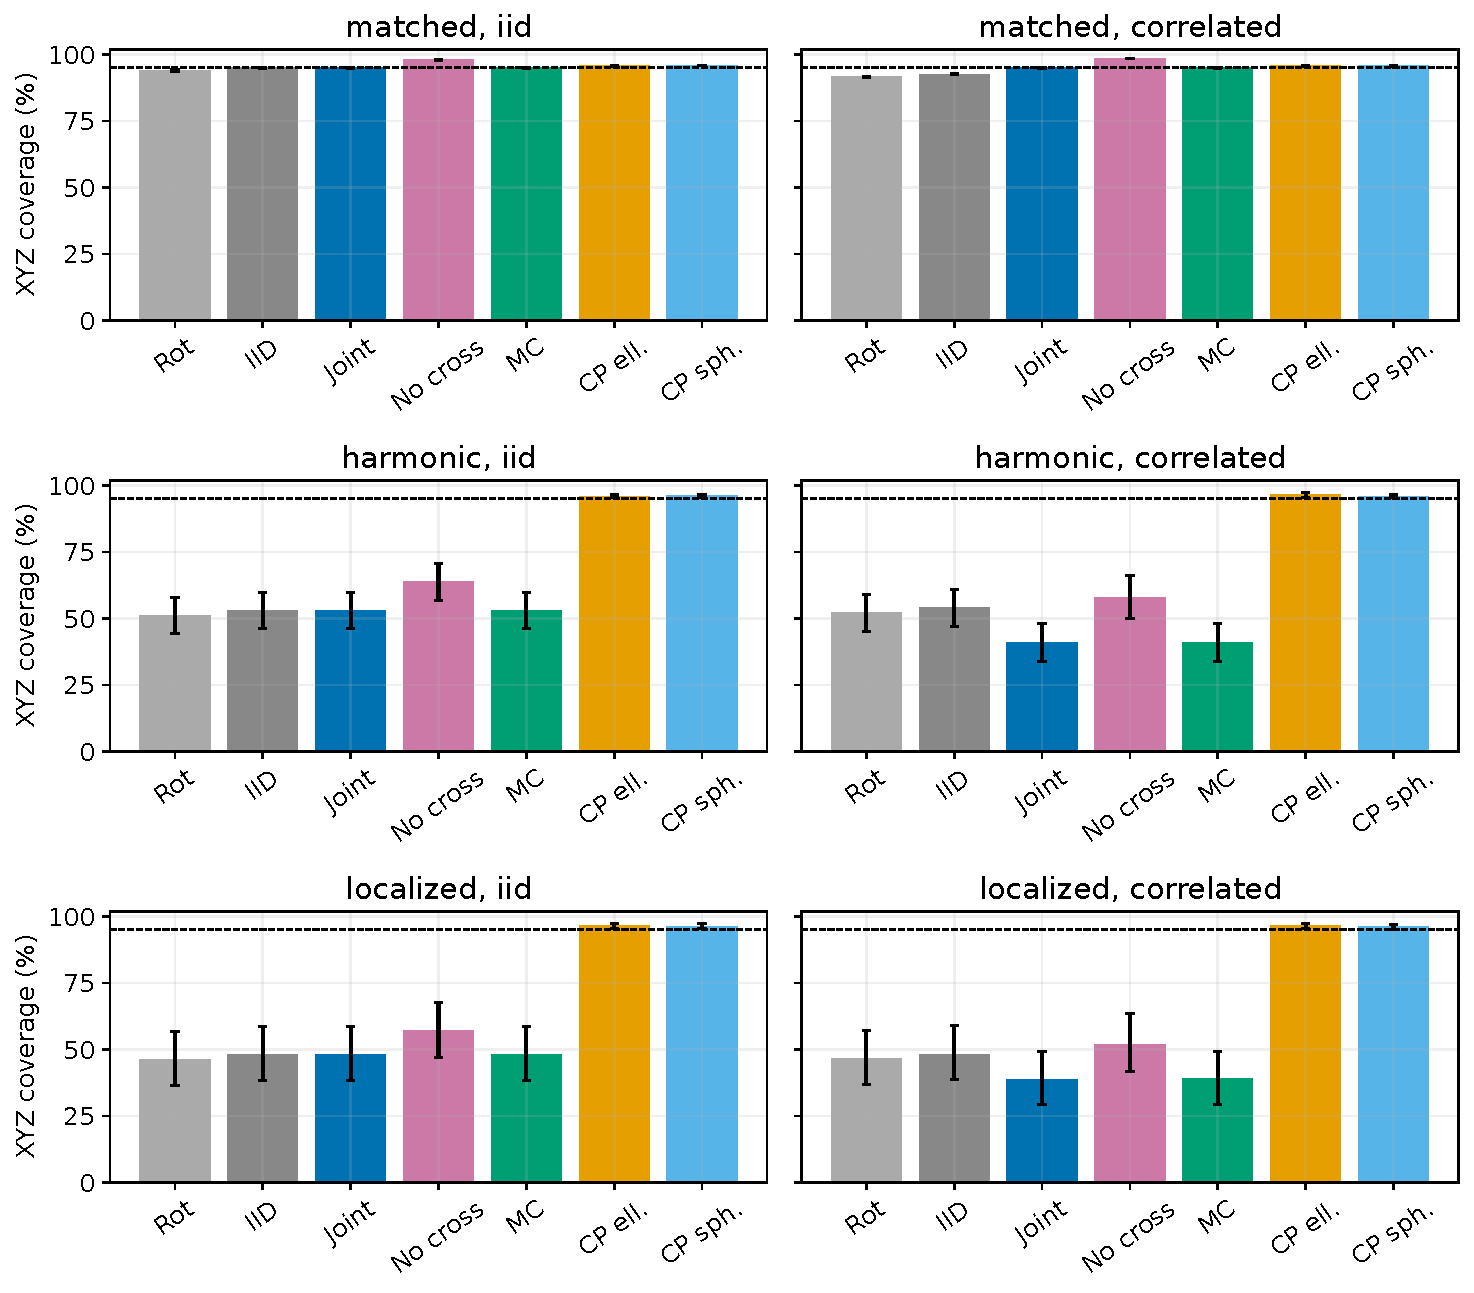
\includegraphics[width=.97\linewidth,height=73mm,keepaspectratio]{figures/audit_region_comparison.pdf}\par\small\refstepcounter{figure}\textbf{Figure \thefigure.} Seven coverage estimates for each family and noise law.\end{center}

\begin{center}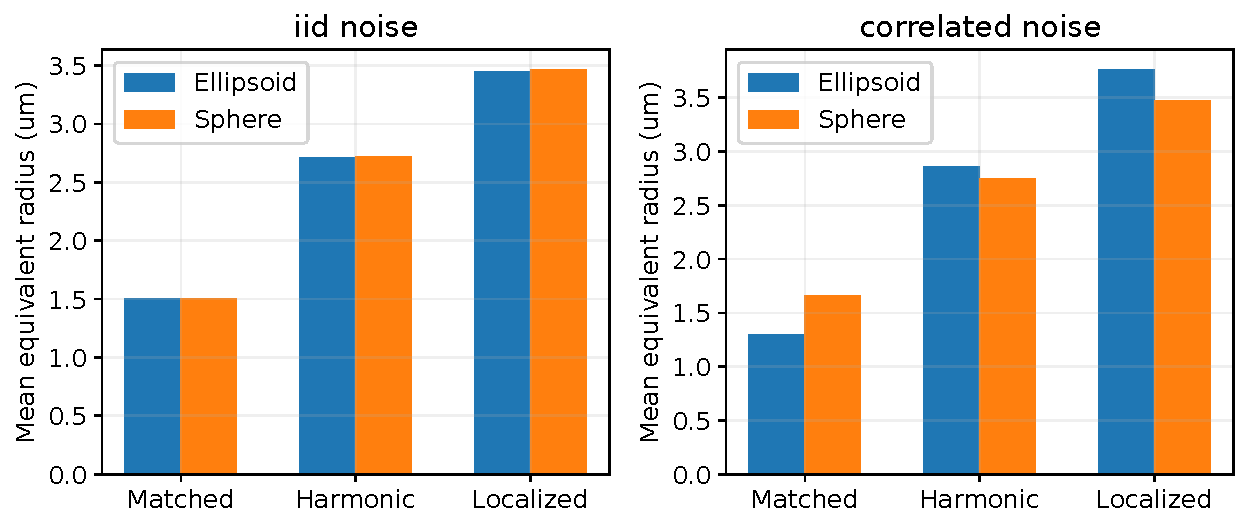
\includegraphics[width=.97\linewidth,height=73mm,keepaspectratio]{figures/audit_region_efficiency.pdf}\par\small\refstepcounter{figure}\textbf{Figure \thefigure.} Equivalent radius for the two response-calibrated shapes.\end{center}

\clearpage

\subsection{State shift and inspection replay}

Fresh calibration measures 96 responses at the original reference poses after adding a fixed displacement. It widens the prediction region while leaving the displacement in place. A complementary inspection replay freezes the normal threshold and marks anomalous responses. A missing vector triggers the acquisition-quality flag before statistical interpretation. The replay plot locates injected spikes in command space; the plotted pose index does not give elapsed time.

\par{\small\textit{Implementation}\quad \file{audit_studies.py}\enspace /\enspace \file{inspection_dashboard.py}}\par

\begin{center}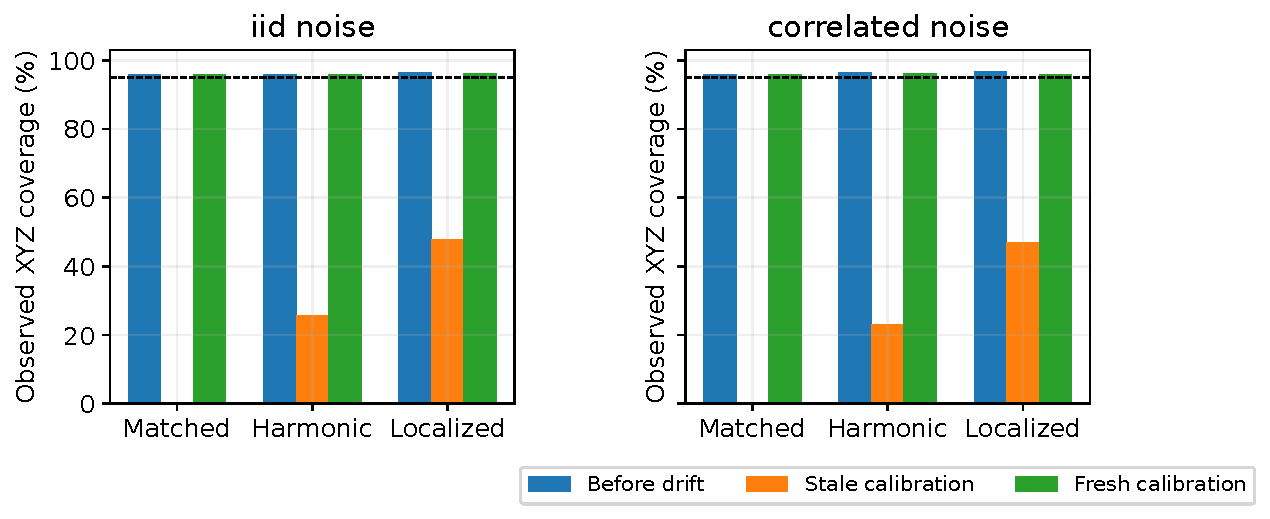
\includegraphics[width=.97\linewidth,height=73mm,keepaspectratio]{figures/audit_drift_coverage.pdf}\par\small\refstepcounter{figure}\textbf{Figure \thefigure.} Before shift, stale calibration and fresh response calibration.\end{center}

\begin{center}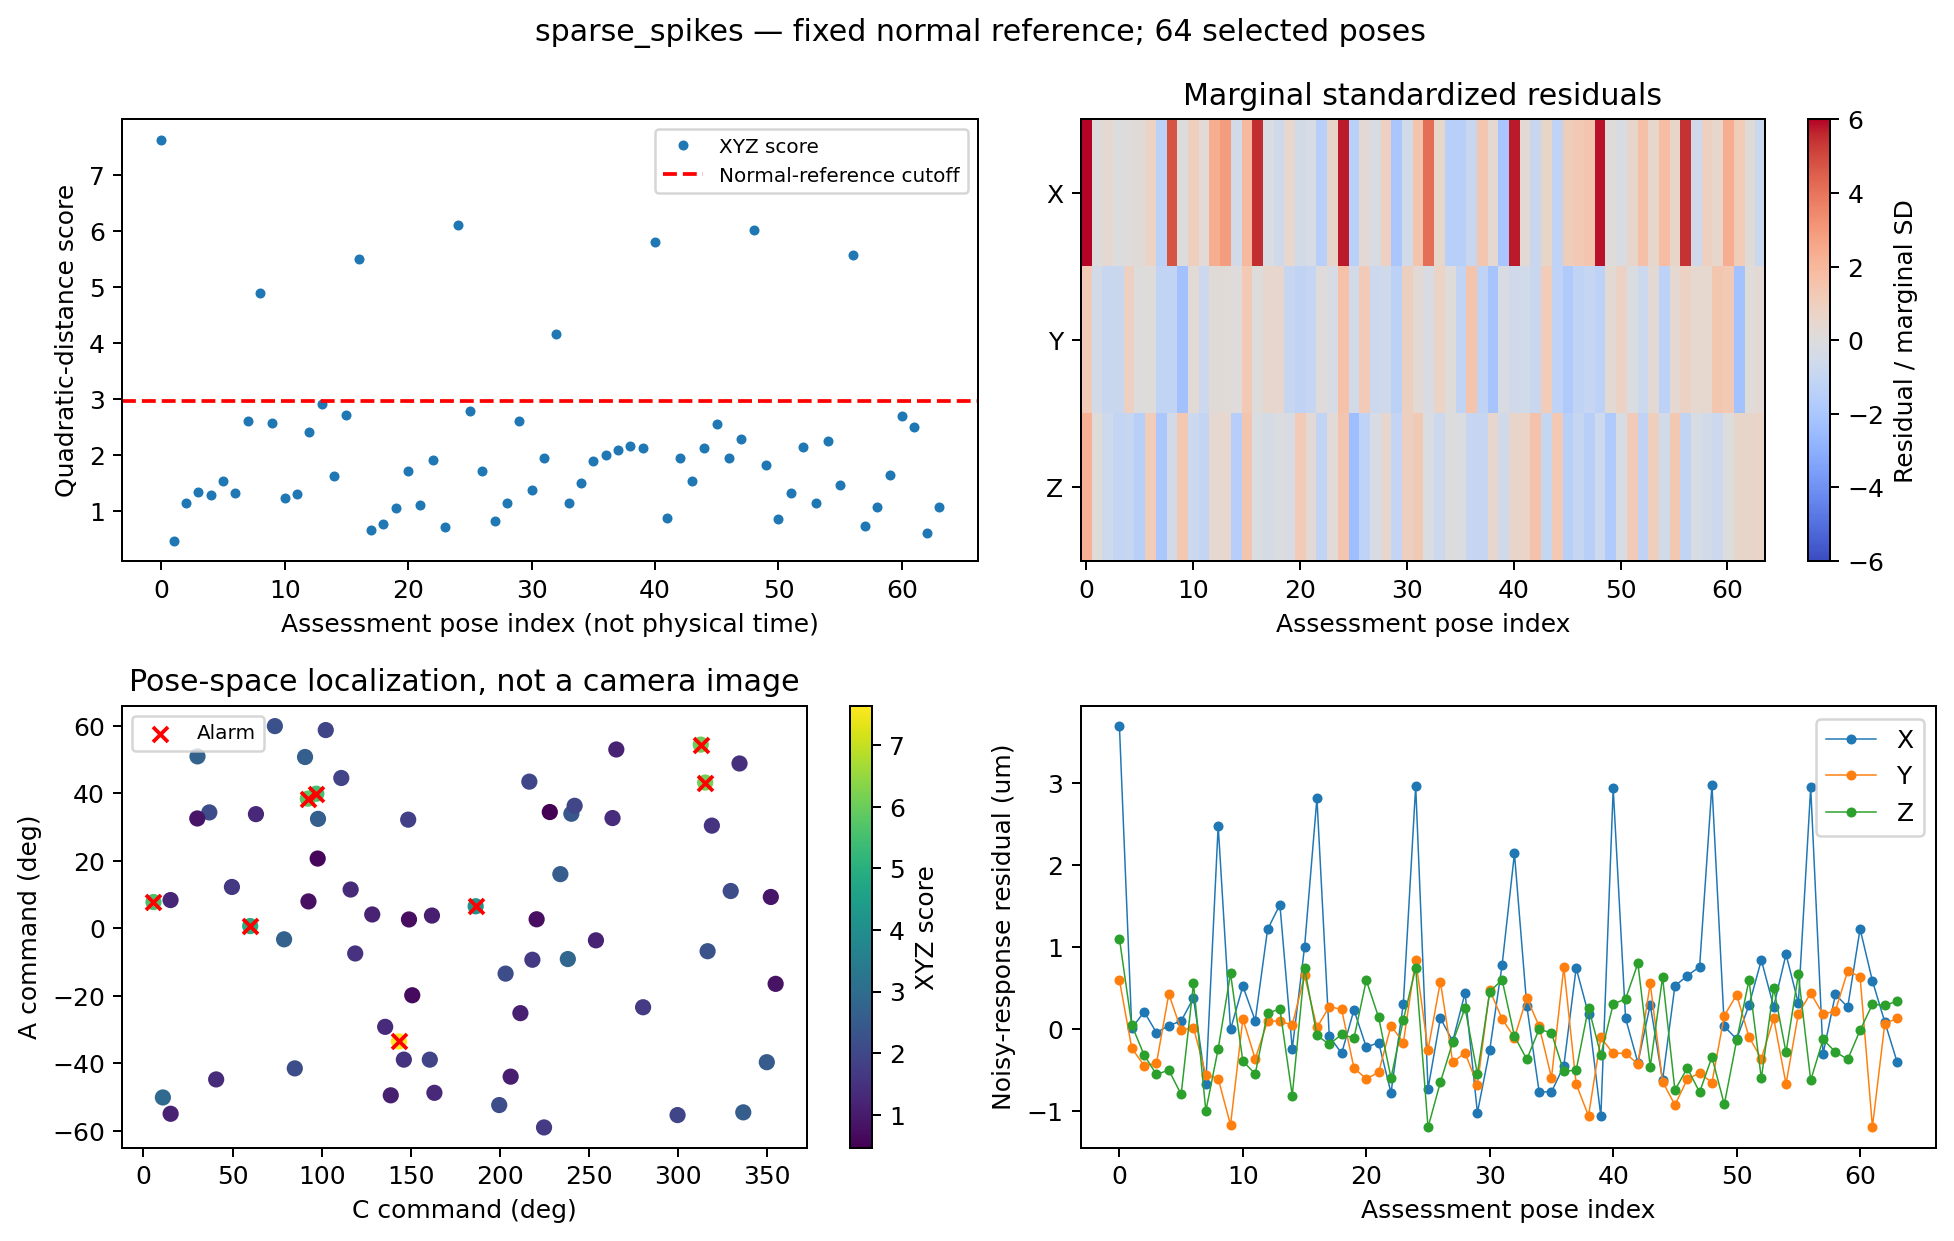
\includegraphics[width=.97\linewidth,height=73mm,keepaspectratio]{figures/inspection_spike_example.png}\par\small\refstepcounter{figure}\textbf{Figure \thefigure.} Stored sparse-spike example with score, standardized residuals and command-space location.\end{center}
\clearpage\section{Numerical outputs by protocol}
\subsection{Calibration design and measurement cost}
The columns below separate total held-out prediction error, its noise-only estimate and the bias measured with exact auxiliary inputs. Task I-optimal selection minimizes a linear prediction-variance criterion over the declared task distribution. That objective gives the smallest tabulated noise term. As omitted geometry grows, changing the selected poses also changes the approximation bias. The second table asks how many distinct poses a scalar-reading budget buys.
\begin{table}[H]\centering\small
\begin{tabular}{llllll}\toprule
Factor & Design & Total RMS & 95\% interval & Noise only & Bias\\\midrule
0 & space filling & 0.194 & 0.188--0.199 & 0.135 & 0.000\\
0 & random & 0.200 & 0.192--0.207 & 0.139 & 0.000\\
0 & d optimal & 0.186 & 0.180--0.192 & 0.125 & 0.000\\
0 & task i optimal & 0.180 & 0.174--0.186 & 0.123 & 0.000\\
1 & space filling & 1.242 & 1.077--1.417 & 0.135 & 1.224\\
1 & random & 1.321 & 1.145--1.506 & 0.139 & 1.300\\
1 & d optimal & 1.244 & 1.074--1.423 & 0.125 & 1.228\\
1 & task i optimal & 1.258 & 1.091--1.435 & 0.123 & 1.241\\
3 & space filling & 3.679 & 3.171--4.211 & 0.135 & 3.672\\
3 & random & 3.911 & 3.372--4.478 & 0.139 & 3.901\\
3 & d optimal & 3.689 & 3.168--4.231 & 0.125 & 3.683\\
3 & task i optimal & 3.731 & 3.223--4.269 & 0.123 & 3.724\\
\bottomrule\end{tabular}\caption{Held-out table displacement-vector RMS at 48 poses / 288 rotary readings, in $\um$. Total RMS resamples PIGEs and rotary noise. Conditional covariance excludes PIGE uncertainty and mismatch. Bias uses exact auxiliary PIGEs.}\label{tab:publication_design_table}\end{table}
\begin{table}[H]\centering\small
\begin{tabular}{lllll}\toprule
Readings & Sensor allocation & Poses & Rank & Noise RMS [$\um$]\\\midrule
96 & position only & 32 & 43 & 0.196\\
96 & position plus angles & 16 & 43 & 0.217\\
168 & position only & 56 & 43 & 0.141\\
168 & position plus angles & 28 & 43 & 0.157\\
288 & position only & 96 & 43 & 0.107\\
288 & position plus angles & 48 & 43 & 0.118\\
\bottomrule\end{tabular}\caption{Equal scalar-reading budgets with task I-optimal selection. Actual acquisition times and instrument costs are not equated.}\label{tab:publication_sensor_table}\end{table}

\clearpage\subsection{Dynamic ablations and sampling interval}
G denotes geometric compensation, T thermal feedforward, B inverse play and F servo feedforward. Read down each clock block to compare schemes on the same motion. Comparing G+B against G alone shows why the two error metrics both matter. In physical time the synchronous TCP error falls, but the normal-plane contour error rises. The lower table is a separate grid-refinement run with fixed estimated time constants.
\begin{table}[H]\centering\small
\begin{tabular}{llll}\toprule
Clock & Scheme & TCP RMS [$\um$] & Normal-plane RMS [$\um$]\\\midrule
physical & uncompensated & 458.45 & 79.38\\
physical & G & 424.15 & 63.77\\
physical & G+F & 44.09 & 18.50\\
physical & G+B & 422.06 & 74.70\\
physical & G+B+F & 40.97 & 13.70\\
physical & G+T & 422.43 & 61.65\\
physical & G+T+F & 43.30 & 19.79\\
physical & G+T+B & 420.26 & 72.41\\
physical & all remedies & 39.38 & 12.87\\
accelerated & uncompensated & 464.07 & 82.61\\
accelerated & G & 430.25 & 70.27\\
accelerated & G+F & 48.79 & 27.04\\
accelerated & G+B & 428.28 & 80.93\\
accelerated & G+B+F & 46.79 & 25.98\\
accelerated & G+T & 423.08 & 66.05\\
accelerated & G+T+F & 49.42 & 31.73\\
accelerated & G+T+B & 420.91 & 76.10\\
accelerated & all remedies & 45.97 & 27.69\\
\bottomrule\end{tabular}\caption{Full factorial reference run: 30 s / 2.5 turns / 0.01 s samples. G: geometry, T: RTDs, B: inverse play, F: feedforward. Physical and accelerated clocks advance 0.5 and 30 min.}\label{tab:publication_dynamic_table}\end{table}
\begin{table}[H]\centering\small
\begin{tabular}{llll}\toprule
Clock & $\Delta t$ [s] & TCP RMS [$\um$] & Normal-plane RMS [$\um$]\\\midrule
physical & 0.04 & 42.452 & 13.644\\
physical & 0.02 & 40.917 & 13.003\\
physical & 0.01 & 39.592 & 12.855\\
physical & 0.005 & 39.431 & 12.840\\
physical & 0.0025 & 39.433 & 12.848\\
physical & 0.00125 & 39.439 & 12.853\\
accelerated & 0.04 & 48.788 & 28.038\\
accelerated & 0.02 & 47.344 & 27.732\\
accelerated & 0.01 & 46.158 & 27.666\\
accelerated & 0.005 & 46.006 & 27.657\\
accelerated & 0.0025 & 46.001 & 27.658\\
accelerated & 0.00125 & 46.005 & 27.660\\
\bottomrule\end{tabular}\caption{Grid sensitivity with fixed fitted lag constants, fixed physical filter time constant and nested RTD noise. Inverse-play discontinuities remain sampling-sensitive.}\label{tab:publication_grid_table}\end{table}

\clearpage\subsection{Model capacity and assessment target}
The larger Fourier and spline fits below each have 67 coefficients. Validation-selected performance includes the cost of 32 additional six-channel validation poses. The lower table concerns a separate, fixed two-harmonic estimator. Changing from a latent target to a noisy observation changes the prediction covariance and the response used to assess it.
\begin{table}[H]\centering\small
\begin{tabular}{lllll}\toprule
Truth family & Model & Parameters & RMS [$\um$] & 95\% interval\\\midrule
harmonic & wrapped cubic & 31 & 7.458 & 6.310--8.687\\
harmonic & fourier2 & 43 & 1.364 & 1.203--1.542\\
harmonic & spline5 & 43 & 1.920 & 1.703--2.163\\
harmonic & fourier4 & 67 & 0.416 & 0.353--0.481\\
harmonic & spline9 & 67 & 0.463 & 0.404--0.519\\
harmonic & validation selected & 67 & 0.417 & 0.353--0.483\\
localized & wrapped cubic & 31 & 7.570 & 6.582--8.831\\
localized & fourier2 & 43 & 1.653 & 1.330--1.969\\
localized & spline5 & 43 & 2.099 & 1.728--2.451\\
localized & fourier4 & 67 & 0.533 & 0.457--0.613\\
localized & spline9 & 67 & 0.597 & 0.497--0.707\\
localized & validation selected & 67 & 0.533 & 0.455--0.617\\
\bottomrule\end{tabular}
\caption{Equal-observation three-turn TCP comparisons. Intervals cluster on error seed with configurations nested. The 43/67-parameter spline and Fourier pairs have equal capacity; the wrapped cubic has 31. Selected models use disjoint noisy rotary validation poses, not TCP assessment truth.}\label{tab:journal_rep}
\end{table}
\begin{table}[H]\centering\small
\begin{tabular}{llllll}\toprule
Case & Rotary & Full & Full+probe & Conformal & CP 95\% interval\\
 & latent & latent & observed & observed & (seed cluster)\\\midrule
matched & 56.13 & 95.56 & 94.97 & 95.75 & 95.59--95.89\\
harmonic mismatch & 0.57 & 5.03 & 53.07 & 96.54 & 96.28--96.83\\
localized mismatch & 0.76 & 5.86 & 45.24 & 95.22 & 93.73--96.38\\
\bottomrule\end{tabular}
\caption{TCP coverage [\%] at nominal 95\%: 12 seeds, 100 noise realizations per case/seed, 96 independent calibration and 64 assessment commands per seed. Latent noise-free TCP and future noisy XYZ-probe responses are different targets. CP denotes split conformal; its ideal rank-based marginal level here is 93/97.}\label{tab:journal_coverage}
\end{table}

\clearpage\subsection{Uncertainty intervals and paired region sizes}
The focused audit pairs methods within each seed. Intervals resample the 12 seed means, retaining the dependence of repeated fits and poses within a seed. The wide interval for localized discrepancy reflects considerable variation across synthetic error maps. The paired radius comparison is in micrometres and measures efficiency at the reported empirical coverage.
\begin{table}[H]\centering\scriptsize
\setlength{\tabcolsep}{3pt}
\begin{tabular}{llrrrr}\toprule
Truth & Noise & Joint & Nonlinear MC & CP ellipsoid & CP sphere\\\midrule
Matched & Independent & 94.98 [94.82, 95.13] & 94.98 [94.82, 95.13] & 95.81 [95.69, 95.93] & 95.86 [95.70, 95.99]\\
Matched & Correlated & 94.97 [94.78, 95.14] & 94.99 [94.80, 95.16] & 95.79 [95.64, 95.93] & 95.84 [95.69, 96.01]\\
Harmonic & Independent & 53.11 [46.24, 59.79] & 53.12 [46.26, 59.80] & 95.97 [95.49, 96.48] & 96.10 [95.63, 96.59]\\
Harmonic & Correlated & 40.98 [33.92, 48.16] & 41.00 [33.95, 48.19] & 96.47 [95.63, 97.24] & 95.96 [95.46, 96.47]\\
Localized & Independent & 47.95 [38.21, 58.73] & 47.95 [38.21, 58.74] & 96.44 [95.37, 97.27] & 96.43 [95.37, 97.26]\\
Localized & Correlated & 38.84 [29.17, 49.05] & 38.88 [29.23, 49.10] & 96.63 [95.54, 97.50] & 96.32 [95.27, 97.10]\\
\bottomrule\end{tabular}
\caption{Observed XYZ coverage [\%] and seed-cluster 95\% intervals. Each cell uses 12 seeds with 100 fits and 64 assessment commands per seed. Gaussian nominal level is 95\%; CP rank level is 95.88\%. The full seven-method records are supplied.}\label{tab:auditcoverage}
\end{table}
\begin{table}[H]\centering\small
\begin{tabular}{llrr}\toprule
Truth & Noise & Radius difference [$\um$] & Paired 95\% interval\\\midrule
Matched & iid & -0.002 & [-0.0039, -0.0001]\\
Matched & correlated & -0.364 & [-0.3711, -0.3590]\\
Harmonic & iid & -0.011 & [-0.0227, -0.0002]\\
Harmonic & correlated & +0.105 & [+0.0404, +0.1685]\\
Localized & iid & -0.012 & [-0.0503, +0.0208]\\
Localized & correlated & +0.282 & [+0.1467, +0.4197]\\
\bottomrule\end{tabular}
\caption{Conformal ellipsoid minus sphere: mean volume-equivalent radius. Negative values favor the ellipsoid by this size metric; positive values favor the sphere. Intervals bootstrap 12 paired seed means.}\label{tab:auditpaired}
\end{table}



\clearpage\subsection{Complete output of the seven-method comparison}Each pair of columns gives coverage in percent and mean volume-equivalent radius in micrometres. The following numbers are calculated from the 50,400 fit-level records using \file{summarize.py}. Within a family and noise law, the point predictions are shared.

\textbf{Matched geometry}

\begin{center}\small\begin{tabular}{@{}lrrrr@{}}\toprule
Method & IID (\%) & Radius & Corr. (\%) & Radius\\\midrule
Rotary only & 93.96 & 1.412 & 91.60 & 1.412\\
Joint, independent assumed & 94.98 & 1.449 & 92.57 & 1.449\\
Joint, correct noise law & 94.98 & 1.449 & 94.97 & 1.251\\
Zero parameter cross terms & 98.05 & 1.651 & 98.54 & 1.516\\
Nonlinear Monte Carlo & 94.98 & 1.449 & 94.99 & 1.251\\
Calibrated ellipsoid & 95.81 & 1.505 & 95.79 & 1.299\\
Calibrated sphere & 95.86 & 1.507 & 95.84 & 1.663\\
\bottomrule\end{tabular}\end{center}

\textbf{Harmonic geometry}

\begin{center}\small\begin{tabular}{@{}lrrrr@{}}\toprule
Method & IID (\%) & Radius & Corr. (\%) & Radius\\\midrule
Rotary only & 51.11 & 1.412 & 52.06 & 1.412\\
Joint, independent assumed & 53.11 & 1.449 & 54.00 & 1.449\\
Joint, correct noise law & 53.11 & 1.449 & 40.98 & 1.251\\
Zero parameter cross terms & 64.04 & 1.651 & 57.91 & 1.516\\
Nonlinear Monte Carlo & 53.12 & 1.449 & 41.00 & 1.251\\
Calibrated ellipsoid & 95.97 & 2.710 & 96.47 & 2.857\\
Calibrated sphere & 96.10 & 2.720 & 95.96 & 2.753\\
\bottomrule\end{tabular}\end{center}

\textbf{Localized geometry}

\begin{center}\small\begin{tabular}{@{}lrrrr@{}}\toprule
Method & IID (\%) & Radius & Corr. (\%) & Radius\\\midrule
Rotary only & 46.14 & 1.412 & 46.53 & 1.412\\
Joint, independent assumed & 47.95 & 1.449 & 48.27 & 1.449\\
Joint, correct noise law & 47.95 & 1.449 & 38.84 & 1.251\\
Zero parameter cross terms & 57.12 & 1.651 & 51.98 & 1.516\\
Nonlinear Monte Carlo & 47.95 & 1.449 & 38.88 & 1.251\\
Calibrated ellipsoid & 96.44 & 3.450 & 96.62 & 3.759\\
Calibrated sphere & 96.43 & 3.462 & 96.32 & 3.477\\
\bottomrule\end{tabular}\end{center}

\clearpage\subsection{State-shift and inspection outputs}Each cell in the first table gives percent coverage / radius in micrometres. A stale threshold leaves the radius fixed as the response distribution moves. The localized case retains more stale coverage because its original regions were already wider. It still falls far below the target after the shift.

\begin{center}\small\begin{tabular}{@{}llrrr@{}}\toprule
Geometry & Noise & Before & Stale & Fresh\\\midrule
Matched & IID & 95.81 / 1.505 & 0.11 / 1.505 & 95.77 / 4.010\\
Matched & Correlated & 95.79 / 1.299 & 0.00 / 1.299 & 95.93 / 4.221\\
Harmonic & IID & 95.97 / 2.710 & 25.70 / 2.710 & 95.87 / 4.864\\
Harmonic & Correlated & 96.47 / 2.857 & 23.19 / 2.857 & 96.26 / 5.460\\
Localized & IID & 96.44 / 3.450 & 47.79 / 3.450 & 96.22 / 5.312\\
Localized & Correlated & 96.62 / 3.759 & 46.86 / 3.759 & 95.94 / 5.914\\
\bottomrule\end{tabular}\end{center}

\medskip\textbf{Inspection notebook replay.} All cases use the same normal-reference threshold. An alarm on a nonfinite measurement is tagged as an acquisition fault. Harmonic and localized cases have no pose-level fault labels; their alarm counts are descriptive.

\begin{center}\small\begin{tabular}{@{}lrrrl@{}}\toprule
Case & Responses & Alarms & Invalid & Labels\\\midrule
normal & 64 & 0 & 0 & yes\\
offset & 64 & 64 & 0 & yes\\
sparse\_spikes & 64 & 8 & 0 & yes\\
dropout & 64 & 8 & 8 & yes\\
harmonic\_mismatch & 64 & 29 & 0 & no\\
localized\_mismatch & 64 & 27 & 0 & no\\
\bottomrule\end{tabular}\end{center}

The eight injected spikes yield eight true positives, 56 true negatives and zero false positives or missed injections. The eight dropouts also trigger eight alarms, all carrying the invalid-reading flag. At 99\% confidence with only 96 calibration scores, the required order exceeds the sample, so the statistical threshold becomes infinite. Missing measurements still trigger the quality flag. An undefined precision or recall is stored as a null value when its denominator is zero.
\clearpage\section{Code excerpts and worked outputs}
\subsection{Axis-tilt inversion}
Subtracting tangential readings at two heights cancels the common translation. The implementation divides by the known height and radius separations. A zero lever arm is rejected before inversion.

\file{calibration.py}
\begin{lstlisting}[language=Python,basicstyle=\scriptsize\ttfamily,breaklines=true]
def a_corrected(read,a,H,H1,L):
    if abs(H1-H)<1e-12 or abs(L)<1e-12: raise ValueError('Need H1!=H and L!=0')
    ra,rr,rt=read.T; s=np.sin(-a); c=np.cos(-a)
    ex=-(rt[1]-rt[0])/(H1-H)
    dy=-s*rr[0]+c*(rt[0]+H*ex)
    dz=c*rr[0]+s*(rt[0]+H*ex)
    dR=(rr[2]-rr[0])/L; dT=(rt[2]-rt[0])/L
    ey=-c*dR-s*dT; ez=-s*dR+c*dT
    dx=ra[0]-H*(c*ey+s*ez)
    return np.array([dx,dy,dz,ex,ey,ez])
\end{lstlisting}
\subsection{Stateful backlash}
The output stays inside a moving interval around the command. On reversal the command must traverse the play band before the output begins to follow in the opposite direction.

\file{remedies.py}
\begin{lstlisting}[language=Python,basicstyle=\scriptsize\ttfamily,breaklines=true]
def play(command,width):
    command=np.asarray(command); out=np.zeros_like(command); out[0]=command[0]
    for k in range(1,len(command)):
        out[k]=np.clip(out[k-1],command[k]-width/2,command[k]+width/2)
    return out
\end{lstlisting}\clearpage
\subsection{Joint uncertainty propagation}
The first contraction forms rotary covariance using a per-pose correlation block. The second contribution propagates the auxiliary uncertainty through K. The final comparison preserves the direct and fitted auxiliary variance but drops their cross terms.

\file{audit_models.py}
\begin{lstlisting}[language=Python,basicstyle=\scriptsize\ttfamily,breaklines=true]
def covariance_variants(base,pinv,channel_correlation):
    P=pinv.reshape(pinv.shape[0],-1,6)
    Cz=np.einsum('ink,kl,jnl->ij',P,channel_correlation,P)
    H,G,K=base['H'],base['G'],base['K'];C=auxiliary_covariance();B=G-K
    rot=np.einsum('nij,jk,nlk->nil',H,Cz,H)
    joint=rot+np.einsum('nij,jk,nlk->nil',K,C,K)
    naive=rot+np.einsum('nij,jk,nlk->nil',G,C,G)+np.einsum('nij,jk,nlk->nil',B,C,B)
    return dict(rotary=rot,joint=joint,naive=naive)
\end{lstlisting}
\subsection{Inspection threshold and acquisition rule}
The array index k minus one converts the mathematical order statistic to Python indexing. Requesting a rank above the available calibration sample returns an infinite statistical cutoff.

\file{inspection_dashboard.py}
\begin{lstlisting}[language=Python,basicstyle=\scriptsize\ttfamily,breaklines=true]
def threshold(scores, alpha=.05):
    scores = np.asarray(scores, dtype=float)
    if scores.ndim != 1 or not len(scores) or not np.isfinite(scores).all():
        raise ValueError('Calibration scores must be a nonempty finite vector')
    if not np.isfinite(alpha) or not 0 < alpha < 1:
        raise ValueError('alpha must be strictly between zero and one')
    k = int(np.ceil((len(scores) + 1) * (1 - alpha)))
    return float(np.partition(scores, k - 1)[k - 1]) if k <= len(scores) else np.inf
\end{lstlisting}
\clearpage\section{Running and reading the project}
\subsection{From a cutter location to a drive command}
The first record of \file{results/example_cl.csv} requests a TCP of $(45,0,20)$ mm with unit direction $(0,-0.529919,0.848048)$. The corresponding first record of \file{results/drive_commands.csv} contains
\[
 (x,y,z,a,c)=(45.032093,10.625698,-133.063877,0.558542,0.000047).
\]
Linear components are in mm and rotary components in rad. The difference between these values and the requested Cartesian coordinates arises from the table orientation, tool length, fixture geometry and fitted correction. The remaining CSV fields give the simulated TCP and angular residuals. This file records numerical commands for the model.

\begin{lstlisting}[language=Python]
from io_tools import load_cl_csv
from summarize import seed_means

p, o = load_cl_csv("results/example_cl.csv")
print(p[0])                         # [45.  0. 20.]
rows = seed_means("audit_region_trials.csv",
                  ["family", "noise_law", "method"])
coverage, radius = rows["matched", "iid", "joint_noise_aware"]
print(f"{coverage:.2%}, {radius:.3f} um")
# 94.98%, 1.449 um
\end{lstlisting}

\subsection{Notebook and script outputs}
\begin{description}
\item[\file{dashboard.py}] Renders the helix and geometric-error controls. The saved \file{helix_animation.html} can be rotated in a browser; its display exaggeration changes the picture only.
\item[\file{research_dashboard.py}] Varies the allocation of calibration poses, their tilt coverage and sensor channels. Its singular values reveal which combinations of errors the sensors can distinguish.
\item[\file{publication_dashboard.py}] Replays the time-domain experiments, including temperature, reversal play, lag and the independent probe.
\item[\file{journal_dashboard.py}] Displays uncertainty regions for the earlier fitted model and permits changes to sensor uncertainty. Its data belong to the earlier journal study.
\item[\file{inspection_dashboard.py}] Produces the alarm map, CSV and six-case JSON summary. In \file{ME3305.ipynb}, the result summary, inspection replay and earlier uncertainty explorer can be run directly from the repository root.
\item[\file{summarize.py} and \file{report_figure.py}] The former reads fit-level coverage and radius and averages within seed, then across seeds. The latter renders the two-panel summary from those records. The underlying fit, plant and covariance modules return arrays to these experiment drivers.
\end{description}
\clearpage\subsection{Verification and how to use the records}
\begin{center}\small\begin{tabular}{@{}p{29mm}rp{99mm}@{}}\toprule
Suite & Checks & What the outputs establish\\\midrule
Baseline & 24 & Rigid-motion exponential against a matrix exponential, inverse/forward consistency at 100 poses, the rotary inverse, sensor projections and standalone remedies.\\
Independent plant & 17 & Agreement of frame and homogeneous evaluations, periodic map seam, pose-design rank and dynamic sensor behaviour.\\
Expanded studies & 16 & Task-design selection, exact two-pole update, model sensitivity, uncertainty arithmetic and dashboard callback.\\
Representation and TCP & 17 & Spline continuity, rank, independent truth implementation, covariance and region explorer.\\
Focused audit & 9 & Batched/scalar equivalence, joint covariance with correlated noise, cross-block removal and scoring safeguards.\\
Inspection & 6 & Finite-sample rank, missing measurement, circular region selection, confusion counts, export and widgets.\\\bottomrule
\end{tabular}\end{center}
A concrete check is the direct matrix-exponential comparison: the baseline verification records a maximum absolute element discrepancy of order $10^{-14}$. The independent geometric implementation checks the frame conventions by computing the same pose in two ways. Neither check supplies a measured machine error. A failed rank check has a different consequence: the available readings cannot identify every coefficient, so a unique estimate with finite covariance would be unjustified.

\textbf{Reading a saved run.} Start with the study's summary JSON to identify the model family, seed and protocol. Use the trial CSV for numerical comparisons, and an NPZ array when the shape of a trajectory or residual matters. For a paired comparison retain the same configuration, seed and noise draw for both methods. \file{OUTPUTS.md} indexes every data file, records the shapes of its arrays or the fields and first row of its CSV, and reproduces the verification records. All raw records are included in the GitHub archive. The report groups repeated stochastic draws into tables and traces to keep the experimental comparisons readable.

\textbf{Output boundaries.} A simulation fit is one realization under a prescribed error map and noise law. Different layers use different numbers of coefficients and poses: the original ballbar identification has 44 parameters, the reference periodic fit has 43 rotary coefficients, and the 65 auxiliary quantities in the uncertainty calculation constitute a separate block. Those counts answer different identification questions. Interactive replays visualize saved cases; the frozen multi-seed records supply the aggregate results.

\clearpage\section{Discussion and conclusions}
\textbf{What the research contributes.} The geometric chain follows the experimentally studied XYZ--AC arrangement of Xiang and Altintas~\cite{xiang}. Design optimization for five-axis calibration and Monte Carlo checks on propagated geometric uncertainty have established precedents~\cite{mchichi,sepahi}. The present project's contribution is a controlled comparison in which the true synthetic geometry, measurement budget and future response are known. Separate controls change the error representation, drive dynamics, measurement dependence or state of the machine, allowing their effects to be examined one at a time where the design permits.
 
\textbf{Interpreting the three outcomes.} A small ballbar residual supports the fitted sensor projection. A small trajectory RMS supports position performance along the tested commands. A high coverage fraction supports a statement about the frequency with which a noisy measurement falls inside its predicted region under the sampled distribution. These three observations require different assessments. In the state-shift experiment, for example, the center of every predicted region stays fixed; the higher coverage comes entirely from a larger threshold.
 
\textbf{What physical measurements would add.} A lab implementation would need a calibrated fixture geometry, identified lever arms, a recorded source for the separate angular channels, and repeated XYZ reference readings independent of fitting. Repeating the assessment across cold and warm sessions would test whether observed shifts persist, whether their direction depends on pose, and whether a re-estimated geometry corrects the position itself.
 
\textbf{Conclusion.}
A periodic rotary model controls multi-turn extrapolation; servo feedforward accounts for much of the improvement on the simulated moving path. Reliable positioning and reliable uncertainty estimates require separate tests. For a physical machine, a direct extension is to fit the geometry in one session and repeat independent XYZ and angular measurements on another day. Reporting both trajectory error and prediction-region radius would show whether a change improved positioning or simply widened the acceptable residual.
\begingroup\small
\begin{thebibliography}{9}\setlength{\itemsep}{0pt}
\bibitem{xiang} S. Xiang and Y. Altintas. Modeling and compensation of volumetric errors for five-axis machine tools. \emph{International Journal of Machine Tools and Manufacture}, 101, 65--78 (2016).
\bibitem{lei} J. Lei et al. Distribution-free predictive inference for regression. \emph{Journal of the American Statistical Association}, 113, 1094--1111 (2018).
\bibitem{mchichi} N. Alami Mchichi and J. R. R. Mayer. Optimal calibration strategy for a five-axis machine tool accuracy improvement using the D-optimal approach. \emph{International Journal of Advanced Manufacturing Technology}, 103, 251--265 (2019).
\bibitem{sepahi} S. Sepahi-Boroujeni, J. R. R. Mayer and F. Khameneifar. Efficient uncertainty estimation of indirectly measured geometric errors of five-axis machine tools via Monte-Carlo validated GUM framework. \emph{Precision Engineering}, 67, 160--171 (2021).
\end{thebibliography}\endgroup
\appendix\clearpage\section{Source-equation implementation index}Equation numbers here refer to Xiang and Altintas~\cite{xiang}. The table records how the project interpreted each source equation and where the corresponding operation is performed. Entries concerning the printed inverse describe the project implementation check.
{\small\begin{longtable}{p{.11\linewidth}p{.42\linewidth}p{.37\linewidth}}
\toprule Paper equations & Derivation / status & Implementation \\\midrule\endhead
(1) & Separate spindle and workpiece product-of-exponential chains & \texttt{Machine.chains} with zero error model \\
(2) & Relative transform by inverse table chain & \texttt{Machine.matrix} \\
(3) & Axis-point velocity gives $v=q\times\omega$ & \texttt{exp\_twist}, rotation helpers \\
(4) & Integrated twist ODE and exact translation & \texttt{exp\_twist} \\
(5) & Rodrigues power-series reduction & \texttt{rx}, rotation exponential \\
(6) & Zero-angular-component translation limit & \texttt{trans}, \texttt{exp\_twist} \\
(7) & Ideal and actual line twists & Axis-line derivation and adjoint; no experimental line data \\
(8) & Exact axis map/logarithm derived; printed pitch form is conditional & General \texttt{exp\_twist}; elementary error factors avoid singular normalization \\
(9) & Parallel-line translation branch & \texttt{trans} \\
(10) & Angular error about a chosen point & \texttt{exp\_twist} with $v=q_e\times u_e$ \\
(11) & C tilt about Y through $(O_x,O_y,O_z)$ & Y error rotation; generic offset twist supported \\
(12) & Ordered six-component axis error motions & \texttt{pdge\_matrix} \\
(13) & Three linear squareness signs & \texttt{ErrorModel.pige\_blocks} \\
(14) & Eight absolute rotary PIGE factors & Same function, absolute convention \\
(15) & All errors inserted at topology-specific positions & \texttt{Machine.chains} \\
(16) & Exact erroneous relative transform & \texttt{Machine.matrix/fk} \\
(17) & Relative eight-PIGE table-ball chain and its linearization & \texttt{table\_exact}, \texttt{table\_sensitivity}, vectorized exact predictor \\
(18) & PDGE cross-product displacement expansion & \texttt{a\_design}, table sensitivities \\
(19) & Relative PIGE displacement terms & First eight table-sensitivity columns \\
(20) & A radial eccentricity offsets & \texttt{piges\_from\_eccentricities} \\
(21) & A axial eccentricity tilts & Same function \\
(22) & C radial combined link terms & Same function \\
(23) & C axial eccentricity tilts & Same function \\
(24) & A axial scalar projection & \texttt{directions}, \texttt{a\_design} \\
(25) & A radial scalar projection & Same functions \\
(26) & A tangential scalar projection & Same functions \\
(27) & Remove PIGE projection before PDGE inversion & Joint/alternating fit residual splitting \\
(28) & Complete A-axis nine-reading observation matrix & \texttt{a\_design}, \texttt{a\_readings} \\
(29) & Literal inverse fails audit; consistent stable inverse derived & \texttt{a\_printed\_eq29}, \texttt{a\_corrected}, symbolic tests \\
(30) & Target-minus-actual position/direction residual & \texttt{compensate} \\
(31) & Cumulative corrected CL command and normalization & \texttt{compensate(method='paper')} \\
(32) & Cubic measured error-map representation & \texttt{ErrorModel.evaluate}, calibration cubic basis \\
(33) & MCS position equals shifted PCS coordinate & \texttt{pcs\_map}, model origin \\
(34) & Datum error subtraction; full frame map also explained & \texttt{pcs\_map}; exact relative matrices \\
(35) & Homogeneous direction with final component zero & \texttt{Machine.fk}, rotation-column extraction \\
(36) & Direction depends on ideal rotary drives only & \texttt{Machine.ik} \\
(37) & Intermediate vector for two rotations & \texttt{paden\_kahan\_orientation} \\
(38) & Intermediate-vector basis expansion & Same function \\
(39) & Projection/norm constraints solve coefficients and branches & Same function \\
(40) & A planar dot/cross angle formula & Same function; AC simplification in \texttt{ik} \\
(41) & C planar angle with inverse-rotation sign & Same function; AC simplification in \texttt{ik} \\
(42) & Ideal forward position from homogeneous origin & \texttt{Machine.fk} with zero error model \\
(43) & Cartesian inverse after selecting rotary angles & \texttt{Machine.ik} \\
(44) & Spindle-side forward chain during RTCP tracking & \texttt{Machine.chains}; nominal sphere follower \\
(45) & Exact inter-sphere length minus nominal length & \texttt{exact\_predictions}, ballbar compensation experiment \\
\bottomrule
\end{longtable}}\end{document}
